\documentclass[8pt,aspectratio=169]{beamer}
\usetheme{Madrid}
\usepackage{graphicx,booktabs,adjustbox,multicol,amsmath,amssymb,listings,xcolor,colortbl}
\definecolor{mlblue}{RGB}{0,102,204}
\definecolor{mlpurple}{RGB}{51,51,178}
\definecolor{mllavender}{RGB}{173,173,224}
\definecolor{mllavender2}{RGB}{193,193,232}
\definecolor{mllavender3}{RGB}{204,204,235}
\definecolor{mllavender4}{RGB}{214,214,239}
\definecolor{mlorange}{RGB}{255,127,14}
\definecolor{mlgreen}{RGB}{44,160,44}
\definecolor{mlred}{RGB}{214,39,40}
\definecolor{mlgray}{RGB}{127,127,127}
% Solidity colors
\definecolor{solkeyword}{RGB}{0,102,153}
\definecolor{solstring}{RGB}{163,21,21}
\definecolor{solcomment}{RGB}{0,128,0}
\definecolor{solnumber}{RGB}{0,128,128}
\setbeamercolor{palette primary}{bg=mllavender3,fg=mlpurple}
\setbeamercolor{palette secondary}{bg=mllavender2,fg=mlpurple}
\setbeamercolor{palette tertiary}{bg=mllavender,fg=white}
\setbeamercolor{palette quaternary}{bg=mlpurple,fg=white}
\setbeamercolor{structure}{fg=mlpurple}
\setbeamercolor{title}{fg=mlpurple}
\setbeamercolor{frametitle}{fg=mlpurple,bg=mllavender3}
\setbeamercolor{block title}{bg=mllavender2,fg=mlpurple}
\setbeamercolor{block body}{bg=mllavender4,fg=black}
\setbeamertemplate{navigation symbols}{}
\setbeamertemplate{itemize items}[circle]
\setbeamersize{text margin left=5mm,text margin right=5mm}
\newcommand{\bottomnote}[1]{\vfill\vspace{-2mm}\textcolor{mllavender2}{\rule{\textwidth}{0.4pt}}\vspace{1mm}\footnotesize\textbf{#1}}
% Solidity language definition
\lstdefinelanguage{Solidity}{
  keywords={pragma, solidity, contract, function, public, private, external, internal, view, pure, payable, returns, return, if, else, for, while, mapping, address, uint, uint256, int, string, bool, bytes, bytes32, event, emit, modifier, require, constructor, memory, storage, calldata, msg, sender, value, this, new, delete, true, false, import, is, constant, override, virtual, interface, library, abstract, struct, enum, unchecked, assembly, abi, encode, decode, keccak256, receive, fallback},
  keywordstyle=\color{solkeyword}\bfseries,
  sensitive=true,
  comment=[l]{//},
  morecomment=[s]{/*}{*/},
  commentstyle=\color{solcomment}\ttfamily,
  stringstyle=\color{solstring}\ttfamily,
  morestring=[b]',
  morestring=[b]"
}
\lstset{language=Solidity,basicstyle=\ttfamily\scriptsize,breaklines=true,frame=single,backgroundcolor=\color{mllavender4},numbers=left,numberstyle=\tiny\color{mlgray},numbersep=5pt,tabsize=2,showstringspaces=false}
\usepackage{tikz,pgfplots}
\pgfplotsset{compat=1.18}
\usetikzlibrary{arrows.meta,positioning,shapes.geometric,calc,chains,decorations.pathmorphing,automata,fit}
\title{Layer 2 Scaling Solutions: Scaling Ethereum and Beyond}
\subtitle{Standalone Technical Lecture}
\author{Prof.~Dr.~Joerg Osterrieder}
\institute{University Lecture Series}
\date{\today}

\begin{document}

%% ============================================================
%% OPENING FRAMES
%% ============================================================

% Frame 1: Title
\begin{frame}
\titlepage
\end{frame}

% Frame 2: Lecture Roadmap
\begin{frame}{Lecture Roadmap}
\begin{columns}[T]
\column{0.55\textwidth}
\vspace{2mm}
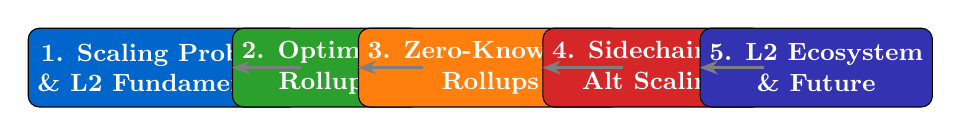
\begin{tikzpicture}[scale=0.9]
  \node[draw,fill=mlblue,text=white,rounded corners=4pt,
        minimum width=2.0cm,minimum height=1.0cm,align=center,font=\small\bfseries]
        (b1) at (0,0) {1. Scaling Problem\\\& L2 Fundamentals};
  \node[draw,fill=mlgreen,text=white,rounded corners=4pt,
        minimum width=2.0cm,minimum height=1.0cm,align=center,font=\small\bfseries]
        (b2) at (2.3,0) {2. Optimistic\\Rollups};
  \node[draw,fill=mlorange,text=white,rounded corners=4pt,
        minimum width=2.0cm,minimum height=1.0cm,align=center,font=\small\bfseries]
        (b3) at (4.6,0) {3. Zero-Knowledge\\Rollups};
  \node[draw,fill=mlred,text=white,rounded corners=4pt,
        minimum width=2.0cm,minimum height=1.0cm,align=center,font=\small\bfseries]
        (b4) at (6.9,0) {4. Sidechains \&\\Alt Scaling};
  \node[draw,fill=mlpurple,text=white,rounded corners=4pt,
        minimum width=2.0cm,minimum height=1.0cm,align=center,font=\small\bfseries]
        (b5) at (9.2,0) {5. L2 Ecosystem\\\& Future};
  \draw[-{Stealth},thick,mlgray] (b1.east) -- (b2.west);
  \draw[-{Stealth},thick,mlgray] (b2.east) -- (b3.west);
  \draw[-{Stealth},thick,mlgray] (b3.east) -- (b4.west);
  \draw[-{Stealth},thick,mlgray] (b4.east) -- (b5.west);
\end{tikzpicture}
\vspace{3mm}

\column{0.45\textwidth}
\begin{block}{Learning Objectives}
\footnotesize
\begin{itemize}
  \item Understand the blockchain trilemma and scalability constraints
  \item Analyse optimistic and zero-knowledge rollup mechanisms
  \item Evaluate state channels, sidechains, and Plasma trade-offs
  \item Assess data availability and proof system designs
  \item Survey the live L2 ecosystem and future directions
\end{itemize}
\end{block}
\vspace{1mm}
\begin{block}{Prerequisites}
\footnotesize
\begin{itemize}
  \item Lessons 1--5: Blockchain fundamentals, smart contracts, DeFi
  \item Basic familiarity with Ethereum and EVM execution
\end{itemize}
\end{block}
\end{columns}
\bottomnote{Duration: 90 minutes | 5 sections | \textasciitilde55 frames | Prerequisite: Lessons 1--5}
\end{frame}

% Frame 3: Table of Contents
\begin{frame}{Table of Contents}
\tableofcontents
\bottomnote{Navigate through 5 sections covering the scaling problem to the L2 ecosystem and future}
\end{frame}

\begin{frame}{Learning Objectives}
By the end of this lecture, you will be able to:
\begin{enumerate}
\item \textbf{Explain} the blockchain trilemma and why Layer 2 scaling is necessary
\item \textbf{Compare} optimistic rollups and ZK rollups (fraud proofs vs.\ validity proofs)
\item \textbf{Analyze} the economics of rollup sequencers, provers, and data availability
\item \textbf{Evaluate} bridge security risks and cross-L2 communication challenges
\item \textbf{Assess} the modular blockchain thesis (execution, settlement, data availability, consensus)
\end{enumerate}
\bottomnote{Bloom's taxonomy levels: Remember $\rightarrow$ Understand $\rightarrow$ Apply $\rightarrow$ Analyze $\rightarrow$ Evaluate $\rightarrow$ Create}
\end{frame}

%% ============================================================
%% SECTION 1: THE SCALING PROBLEM & LAYER 2 FUNDAMENTALS
%% ============================================================
\section{The Scaling Problem \& Layer 2 Fundamentals}

% Frame 4: Section 1 Divider
\begin{frame}{}
\begin{beamercolorbox}[sep=12pt,center,rounded=true,shadow=true]{palette quaternary}
  {\Large\bfseries Section 1: The Scaling Problem \& Layer 2 Fundamentals}\\[6pt]
  {\normalsize Why blockchains can't scale natively and how Layer 2 solves it}
\end{beamercolorbox}
\vspace{4mm}
\begin{columns}[T]
\column{0.5\textwidth}
\begin{block}{What You Will Learn}
\footnotesize
\begin{itemize}
  \item The blockchain trilemma and its implications for scalability
  \item Why Ethereum L1 is limited to \textasciitilde15 TPS
  \item Layer 2 taxonomy: rollups, state channels, sidechains, validiums
  \item State channels, Plasma, and early L2 approaches
\end{itemize}
\end{block}
\column{0.5\textwidth}
\begin{block}{Frames in This Section}
\footnotesize
\begin{itemize}
  \item Frame 5: The Blockchain Trilemma
  \item Frame 6: Ethereum's Scaling Bottleneck
  \item Frame 7: L2 Taxonomy Overview
  \item Frame 8: State Channel Contract (Code)
  \item Frame 9: State Channels Deep Dive
  \item Frame 10: Plasma Chains
  \item Frame 11: Rollups vs Other L2 Approaches
  \item Frame 12: How Rollups Work (General)
  \item Frame 13: Data Compression in Rollups
  \item Frame 14: Section 1 Summary
\end{itemize}
\end{block}
\end{columns}
\bottomnote{Section 1 of 5 | Frames 4--14}
\end{frame}

% Frame 5: The Blockchain Trilemma
\begin{frame}{The Blockchain Trilemma}
\begin{columns}[T]
\column{0.55\textwidth}
\vspace{2mm}
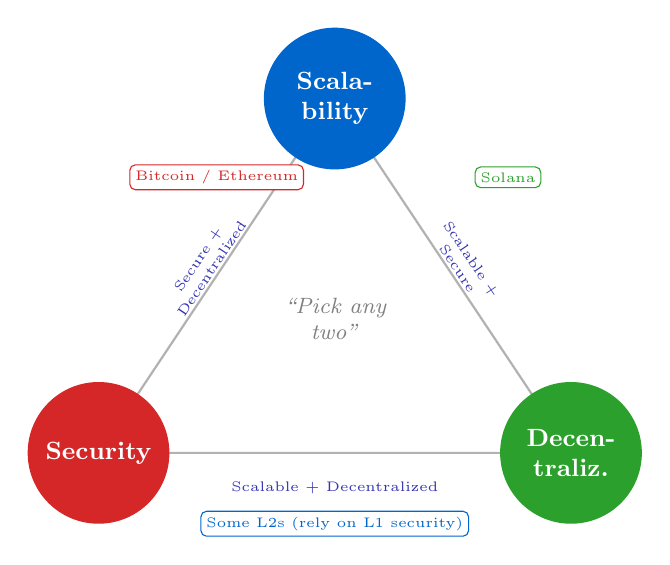
\begin{tikzpicture}[scale=1.0]
  % Triangle vertices
  \coordinate (top)   at (3.0, 5.0);
  \coordinate (botL)  at (0.0, 0.5);
  \coordinate (botR)  at (6.0, 0.5);
  % Triangle edges
  \draw[thick,mlgray!60] (top) -- (botL) -- (botR) -- cycle;
  % Vertex circles
  \node[circle,fill=mlblue,text=white,minimum size=1.8cm,align=center,font=\small\bfseries]
    at (top)  {Scala-\\bility};
  \node[circle,fill=mlred,text=white,minimum size=1.8cm,align=center,font=\small\bfseries]
    at (botL) {Security};
  \node[circle,fill=mlgreen,text=white,minimum size=1.8cm,align=center,font=\small\bfseries]
    at (botR) {Decen-\\traliz.};
  % Center label
  \node[align=center,font=\footnotesize\itshape,text=mlgray]
    at (3.0, 2.2) {``Pick any\\two''};
  % Edge annotations
  \node[align=center,font=\tiny,text=mlpurple,rotate=56]
    at (1.35, 2.9) {Secure +\\Decentralized};
  \node[align=center,font=\tiny,text=mlpurple,rotate=-56]
    at (4.65, 2.9) {Scalable +\\Secure};
  \node[align=center,font=\tiny,text=mlpurple]
    at (3.0, 0.05) {Scalable + Decentralized};
  % Example labels
  \node[align=center,font=\tiny,text=mlred,fill=white,rounded corners=2pt,
        draw=mlred,inner sep=2pt] at (1.5, 4.0)
    {Bitcoin / Ethereum};
  \node[align=center,font=\tiny,text=mlgreen,fill=white,rounded corners=2pt,
        draw=mlgreen,inner sep=2pt] at (5.2, 4.0)
    {Solana};
  \node[align=center,font=\tiny,text=mlblue,fill=white,rounded corners=2pt,
        draw=mlblue,inner sep=2pt] at (3.0, -0.4)
    {Some L2s (rely on L1 security)};
\end{tikzpicture}
\column{0.45\textwidth}
\vspace{4mm}
\begin{block}{The Trilemma Explained}
\footnotesize
\begin{itemize}
  \item \textbf{Scalability}: High throughput, low latency, low fees
  \item \textbf{Security}: Resistant to attacks; honest-minority assumption
  \item \textbf{Decentralization}: No single point of control or failure
\end{itemize}
\end{block}
\vspace{2mm}
\begin{block}{Implications}
\footnotesize
\begin{itemize}
  \item Optimizing two properties degrades the third
  \item Ethereum chose security + decentralization
  \item Result: \textasciitilde15 TPS, high gas fees at peak demand
  \item Layer 2 aims to \textit{break} the trilemma by moving execution off-chain while settling on L1
\end{itemize}
\end{block}
\end{columns}
\bottomnote{Vitalik Buterin formalized the trilemma -- Layer 2 solutions aim to break it by separating execution from consensus}
\end{frame}

% Frame 6: Ethereum's Scaling Bottleneck
\begin{frame}{Ethereum's Scaling Bottleneck}
\begin{columns}[T]
\column{0.45\textwidth}
\begin{block}{Hard Limits at L1}
\footnotesize
\begin{itemize}
  \item \textbf{\textasciitilde15 TPS} -- theoretical maximum under normal load
  \item \textbf{Block gas limit}: 30M gas (target 15M after EIP-1559)
  \item \textbf{Simple transfer}: 21,000 gas
  \item \textbf{DEX swap}: \textasciitilde150,000 gas
  \item \textbf{Complex DeFi tx}: 200,000--500,000 gas
\end{itemize}
\end{block}
\vspace{2mm}
\begin{block}{Economic Consequences}
\footnotesize
\begin{itemize}
  \item Peak demand: base fee spikes to 100+ gwei
  \item Gas cost: \$50--\$500 per transaction at peaks
  \item NFT mint frenzies: gas wars drove fees to \$1,000+
  \item DeFi Summer 2020 congestion: weeks of 100+ gwei
  \item Blocks fill in milliseconds; users outbid each other
\end{itemize}
\end{block}
\vspace{2mm}
\begin{alertblock}{The Comparison}
\footnotesize
Ethereum: \textasciitilde1.3M tx/day\\
Visa: \textasciitilde150M tx/day (115$\times$ more)
\end{alertblock}
\column{0.55\textwidth}
\vspace{1mm}
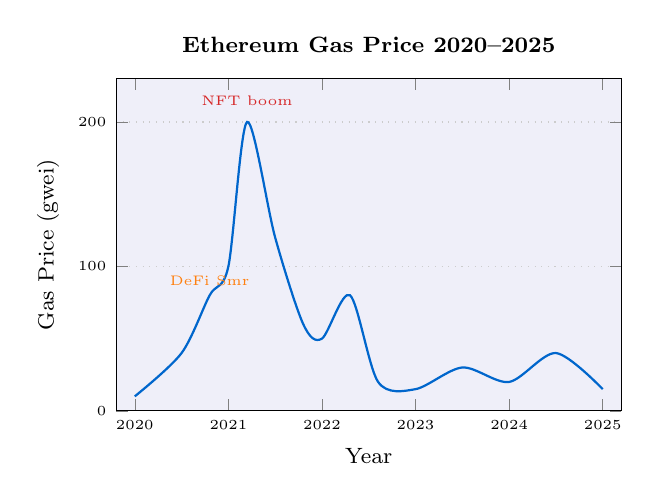
\begin{tikzpicture}
\begin{axis}[
  width=8.0cm, height=5.8cm,
  xlabel={\footnotesize Year},
  ylabel={\footnotesize Gas Price (gwei)},
  title={\footnotesize\bfseries Ethereum Gas Price 2020--2025},
  xtick={2020,2021,2022,2023,2024,2025},
  xticklabels={2020,2021,2022,2023,2024,2025},
  xticklabel style={font=\tiny},
  yticklabel style={font=\tiny},
  title style={font=\footnotesize\bfseries},
  xlabel style={font=\footnotesize},
  ylabel style={font=\footnotesize},
  ymajorgrids=true,
  grid style={dotted,mlgray!40},
  axis background/.style={fill=mllavender4!40},
  xmin=2019.8, xmax=2025.2,
  ymin=0, ymax=230,
]
% Approximate historical gas price curve
\addplot[thick,mlblue,smooth] coordinates {
  (2020.0, 10)
  (2020.5, 40)
  (2020.8, 80)   % DeFi Summer
  (2021.0, 100)
  (2021.2, 200)  % NFT / Bull market peak
  (2021.5, 120)
  (2021.8, 60)
  (2022.0, 50)
  (2022.3, 80)   % Luna collapse
  (2022.6, 20)
  (2023.0, 15)
  (2023.5, 30)   % Ordinals / L1 traffic
  (2024.0, 20)
  (2024.5, 40)   % EIP-4844 blobs reduce pressure
  (2025.0, 15)
};
% Spike annotations
\node[font=\tiny,text=mlred,align=center] at (axis cs:2021.2,215)
  {NFT boom};
\node[font=\tiny,text=mlorange,align=center] at (axis cs:2020.8,90)
  {DeFi Smr};
\end{axis}
\end{tikzpicture}
\end{columns}
\bottomnote{At 15 TPS, Ethereum can serve roughly 1.3 million transactions per day -- Visa processes 150 million}
\end{frame}

% Frame 7: L2 Taxonomy Overview
\begin{frame}{L2 Taxonomy Overview}
\vspace{-1mm}
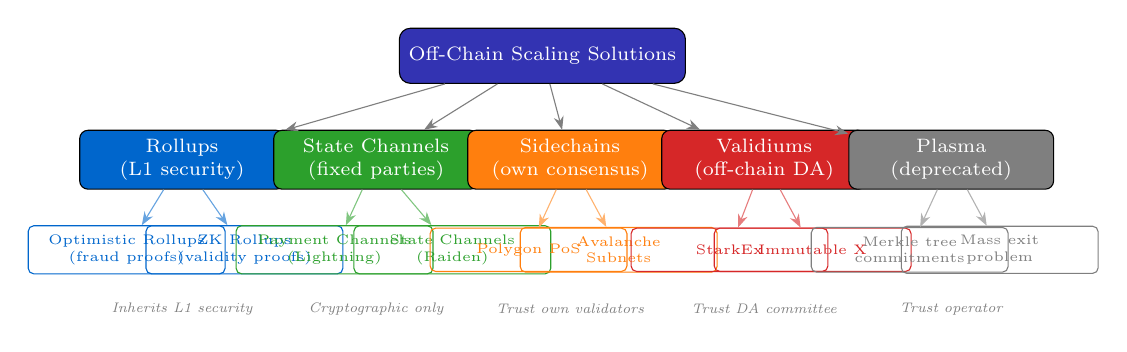
\begin{tikzpicture}[
  scale=0.88,
  every node/.style={font=\scriptsize},
  root/.style={draw,fill=mlpurple,text=white,rounded corners=4pt,
               minimum width=3.2cm,minimum height=0.7cm,align=center},
  branch/.style={draw,rounded corners=3pt,minimum width=2.6cm,
                 minimum height=0.65cm,align=center,text=white},
  leaf/.style={draw,rounded corners=2pt,minimum width=2.5cm,
               minimum height=0.55cm,align=center,font=\tiny},
  trust/.style={font=\tiny\itshape,text=mlgray},
]
  % Root
  \node[root] (root) at (6.0, 4.5) {Off-Chain Scaling Solutions};

  % Branch nodes
  \node[branch,fill=mlblue]    (rollups)    at (0.8,  3.0) {Rollups\\(L1 security)};
  \node[branch,fill=mlgreen]   (schan)      at (3.6,  3.0) {State Channels\\(fixed parties)};
  \node[branch,fill=mlorange]  (side)       at (6.4,  3.0) {Sidechains\\(own consensus)};
  \node[branch,fill=mlred]     (valid)      at (9.2,  3.0) {Validiums\\(off-chain DA)};
  \node[branch,fill=mlgray]    (plasma)     at (11.9, 3.0) {Plasma\\(deprecated)};

  % Arrows root -> branches
  \draw[-{Stealth},mlgray] (root) -- (rollups);
  \draw[-{Stealth},mlgray] (root) -- (schan);
  \draw[-{Stealth},mlgray] (root) -- (side);
  \draw[-{Stealth},mlgray] (root) -- (valid);
  \draw[-{Stealth},mlgray] (root) -- (plasma);

  % Rollup leaves
  \node[leaf,draw=mlblue,text=mlblue]  (orb) at (0.0, 1.7) {Optimistic Rollups\\(fraud proofs)};
  \node[leaf,draw=mlblue,text=mlblue]  (zkr) at (1.7, 1.7) {ZK Rollups\\(validity proofs)};
  \draw[-{Stealth},mlblue!60] (rollups) -- (orb);
  \draw[-{Stealth},mlblue!60] (rollups) -- (zkr);

  % State channel leaves
  \node[leaf,draw=mlgreen,text=mlgreen] (pay) at (3.0, 1.7) {Payment Channels\\(Lightning)};
  \node[leaf,draw=mlgreen,text=mlgreen] (rai) at (4.7, 1.7) {State Channels\\(Raiden)};
  \draw[-{Stealth},mlgreen!60] (schan) -- (pay);
  \draw[-{Stealth},mlgreen!60] (schan) -- (rai);

  % Sidechain leaves
  \node[leaf,draw=mlorange,text=mlorange] (pol) at (5.8, 1.7) {Polygon PoS};
  \node[leaf,draw=mlorange,text=mlorange] (ava) at (7.1, 1.7) {Avalanche\\Subnets};
  \draw[-{Stealth},mlorange!60] (side) -- (pol);
  \draw[-{Stealth},mlorange!60] (side) -- (ava);

  % Validium leaves
  \node[leaf,draw=mlred,text=mlred] (sex) at (8.7, 1.7) {StarkEx};
  \node[leaf,draw=mlred,text=mlred] (imx) at (9.9, 1.7) {Immutable X};
  \draw[-{Stealth},mlred!60] (valid) -- (sex);
  \draw[-{Stealth},mlred!60] (valid) -- (imx);

  % Plasma leaves
  \node[leaf,draw=mlgray,text=mlgray] (plx) at (11.3, 1.7) {Merkle tree\\commitments};
  \node[leaf,draw=mlgray,text=mlgray] (mep) at (12.6, 1.7) {Mass exit\\problem};
  \draw[-{Stealth},mlgray!60] (plasma) -- (plx);
  \draw[-{Stealth},mlgray!60] (plasma) -- (mep);

  % Trust model annotations
  \node[trust] at (0.8,  0.85) {Inherits L1 security};
  \node[trust] at (3.6,  0.85) {Cryptographic only};
  \node[trust] at (6.4,  0.85) {Trust own validators};
  \node[trust] at (9.2,  0.85) {Trust DA committee};
  \node[trust] at (11.9, 0.85) {Trust operator};
\end{tikzpicture}
\bottomnote{Rollups are the dominant paradigm because they inherit L1 security while supporting general-purpose computation}
\end{frame}

% Frame 8: State Channel Contract [FRAGILE] -- CODE FRAME 1
\begin{frame}[fragile]{State Channel Contract}
\begin{columns}[T]
\column{0.50\textwidth}
\vspace{1mm}
\begin{lstlisting}[language=Solidity,caption={Simple Payment Channel}]
// Simple Payment Channel
contract PaymentChannel {
    address public sender;
    address public recipient;
    uint256 public expiration;

    constructor(address _to,
                uint256 duration)
        payable {
        sender = msg.sender;
        recipient = _to;
        expiration = block.timestamp
            + duration;
    }

    function close(uint256 amount,
                   bytes memory sig)
        external {
        require(msg.sender == recipient);
        require(verify(amount, sig));
        payable(recipient).transfer(
            amount);
        selfdestruct(
            payable(sender));
    }
}
\end{lstlisting}
\column{0.50\textwidth}
\vspace{2mm}
\begin{block}{How State Channels Work}
\footnotesize
\begin{itemize}
  \item \textbf{Open}: Sender deposits ETH into the contract (1 on-chain tx)
  \item \textbf{Transact}: Parties exchange signed messages off-chain -- no gas, instant finality
  \item \textbf{Close}: Recipient submits final signed state; contract verifies and distributes (1 on-chain tx)
  \item \textbf{Dispute}: If sender stops responding, recipient can close after \texttt{expiration}
\end{itemize}
\end{block}
\vspace{2mm}
\begin{block}{Key Properties}
\footnotesize
\begin{itemize}
  \item Only 2 on-chain transactions regardless of how many off-chain messages
  \item Privacy: intermediate states never touch the chain
  \item Limitation: participants must be known in advance; capital locked for channel lifetime
  \item Best for: micropayments, gaming, repeated bilateral interactions
\end{itemize}
\end{block}
\end{columns}
\bottomnote{State channels are ideal for repeated payments between two parties -- e.g., micropayments, gaming moves}
\end{frame}

% Frame 9: State Channels Deep Dive
\begin{frame}{State Channels Deep Dive}
\begin{columns}[T]
\column{0.58\textwidth}
\vspace{1mm}
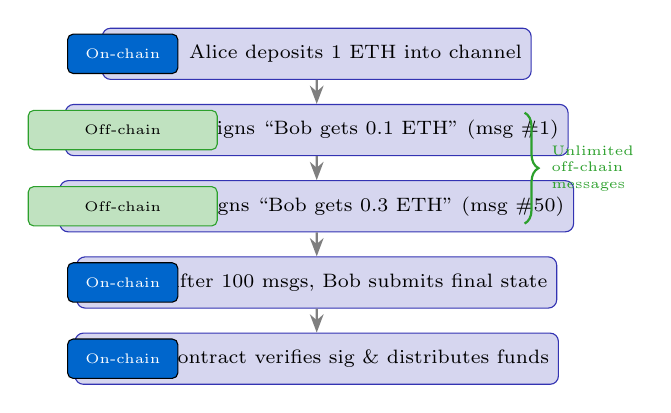
\begin{tikzpicture}[
  scale=0.88,
  every node/.style={font=\scriptsize},
  stepbox/.style={draw,rounded corners=3pt,minimum width=3.2cm,
                  minimum height=0.65cm,align=center,fill=mllavender4,draw=mlpurple},
  onchain/.style={draw,rounded corners=2pt,minimum width=1.4cm,
                  minimum height=0.5cm,align=center,fill=mlblue,text=white,font=\tiny},
  offchain/.style={draw,rounded corners=2pt,minimum width=2.4cm,
                   minimum height=0.5cm,align=center,fill=mlgreen!30,
                   draw=mlgreen,font=\tiny},
  arr/.style={-{Stealth},thick,mlgray},
]
  % Steps
  \node[stepbox] (s1) at (3.5, 5.0)
    {Step 1: Alice deposits 1 ETH into channel};
  \node[stepbox] (s2) at (3.5, 3.9)
    {Step 2: Alice signs ``Bob gets 0.1 ETH'' (msg \#1)};
  \node[stepbox] (s3) at (3.5, 2.8)
    {Step 3: Alice signs ``Bob gets 0.3 ETH'' (msg \#50)};
  \node[stepbox] (s4) at (3.5, 1.7)
    {Step 4: After 100 msgs, Bob submits final state};
  \node[stepbox] (s5) at (3.5, 0.6)
    {Step 5: Contract verifies sig \& distributes funds};

  % Badges
  \node[onchain]  at (0.7, 5.0) {On-chain};
  \node[offchain] at (0.7, 3.9) {Off-chain};
  \node[offchain] at (0.7, 2.8) {Off-chain};
  \node[onchain]  at (0.7, 1.7) {On-chain};
  \node[onchain]  at (0.7, 0.6) {On-chain};

  % Arrows
  \draw[arr] (s1) -- (s2);
  \draw[arr] (s2) -- (s3);
  \draw[arr] (s3) -- (s4);
  \draw[arr] (s4) -- (s5);

  % Brace annotation
  \draw[decorate,decoration={brace,amplitude=5pt},mlgreen,thick]
    (6.5, 4.15) -- (6.5, 2.55)
    node[midway,right=6pt,align=left,font=\tiny,text=mlgreen]
      {Unlimited\\off-chain\\messages};
\end{tikzpicture}
\column{0.42\textwidth}
\vspace{4mm}
\begin{block}{Economics}
\footnotesize
\begin{itemize}
  \item \textbf{2 on-chain txs}: open + close
  \item \textbf{Unlimited} off-chain transactions
  \item No gas for intermediate states
  \item Capital locked for channel duration
\end{itemize}
\end{block}
\vspace{2mm}
\begin{block}{Lightning Network (Bitcoin)}
\footnotesize
\begin{itemize}
  \item 5,000+ BTC locked capacity
  \item \textasciitilde16,000 routing nodes
  \item Millisecond payment finality
  \item Multi-hop routing via HTLCs
\end{itemize}
\end{block}
\vspace{2mm}
\begin{block}{Raiden Network (Ethereum)}
\footnotesize
\begin{itemize}
  \item ERC-20 payment channels
  \item Same HTLC routing model
  \item Less adoption than Lightning
\end{itemize}
\end{block}
\end{columns}
\bottomnote{State channels achieve unlimited throughput between two parties with only 2 on-chain transactions total}
\end{frame}

% Frame 10: Plasma Chains
\begin{frame}{Plasma Chains}
\begin{columns}[T]
\column{0.48\textwidth}
\begin{block}{Plasma Architecture}
\footnotesize
\begin{itemize}
  \item \textbf{Child chains} run independently with their own operators and blocks
  \item Child chain operators periodically \textbf{commit Merkle roots} to L1
  \item Users can \textbf{exit} with a Merkle proof showing their funds on the child chain
  \item L1 enforces exit validity through a \textbf{challenge period} (typically 7 days)
\end{itemize}
\end{block}
\vspace{2mm}
\begin{alertblock}{Why Plasma Failed}
\footnotesize
\begin{itemize}
  \item \textbf{Mass exit problem}: if operator turns malicious, all users must exit simultaneously -- L1 cannot process them all
  \item \textbf{Data availability}: operator can withhold block data, preventing users from constructing valid exit proofs
  \item \textbf{Limited generality}: complex smart contract logic is difficult to prove in exit games
\end{itemize}
\end{alertblock}
\column{0.52\textwidth}
\vspace{1mm}
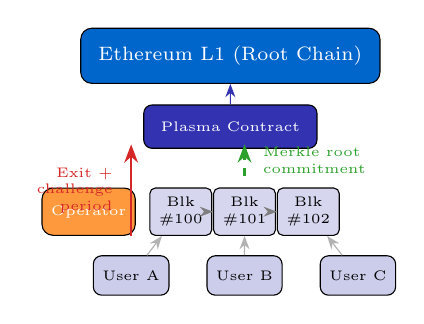
\begin{tikzpicture}[
  scale=0.9,
  every node/.style={font=\scriptsize},
  l1box/.style={draw,fill=mlblue,text=white,rounded corners=4pt,
                minimum width=3.8cm,minimum height=0.7cm,align=center},
  plasmabox/.style={draw,fill=mlorange!80,text=white,rounded corners=4pt,
                    minimum width=1.1cm,minimum height=0.6cm,align=center,font=\tiny},
  blockbox/.style={draw,fill=mllavender4,rounded corners=2pt,
                   minimum width=0.7cm,minimum height=0.55cm,align=center,font=\tiny},
]
  % L1
  \node[l1box] (l1) at (3.2, 4.8) {Ethereum L1 (Root Chain)};

  % Plasma contract on L1
  \node[draw,fill=mlpurple,text=white,rounded corners=3pt,
        minimum width=2.2cm,minimum height=0.55cm,align=center,font=\tiny]
    (plcon) at (3.2, 3.8) {Plasma Contract};
  \draw[-{Stealth},mlpurple] (plcon) -- (l1);

  % Plasma child chain
  \node[plasmabox] (op) at (1.2, 2.6) {Operator};
  \node[blockbox]  (blA) at (2.5, 2.6) {Blk\\\#100};
  \node[blockbox]  (blB) at (3.4, 2.6) {Blk\\\#101};
  \node[blockbox]  (blC) at (4.3, 2.6) {Blk\\\#102};
  \draw[-{Stealth},mlgray] (blA) -- (blB);
  \draw[-{Stealth},mlgray] (blB) -- (blC);

  % Merkle root commitment arrow
  \draw[-{Stealth},dashed,mlgreen,thick]
    (3.4, 3.1) -- (3.4, 3.55)
    node[midway,right=3pt,font=\tiny,text=mlgreen,align=left]
      {Merkle root\\commitment};

  % User exit arrow
  \draw[-{Stealth},mlred,thick]
    (1.8, 2.25) -- (1.8, 3.55)
    node[midway,left=3pt,font=\tiny,text=mlred,align=right]
      {Exit +\\challenge\\period};

  % Users at bottom
  \node[draw,fill=mllavender3,rounded corners=3pt,
        minimum width=0.8cm,minimum height=0.5cm,align=center,font=\tiny]
    (ua) at (1.8, 1.7) {User A};
  \node[draw,fill=mllavender3,rounded corners=3pt,
        minimum width=0.8cm,minimum height=0.5cm,align=center,font=\tiny]
    (ub) at (3.4, 1.7) {User B};
  \node[draw,fill=mllavender3,rounded corners=3pt,
        minimum width=0.8cm,minimum height=0.5cm,align=center,font=\tiny]
    (uc) at (5.0, 1.7) {User C};

  \draw[-{Stealth},mlgray!60] (ua) -- (blA);
  \draw[-{Stealth},mlgray!60] (ub) -- (blB);
  \draw[-{Stealth},mlgray!60] (uc) -- (blC);
\end{tikzpicture}
\vspace{-1mm}
\begin{block}{Historical Note}
\footnotesize
Plasma proposed 2017 (Buterin \& Poon); superseded by rollups which solve the data availability problem elegantly
\end{block}
\end{columns}
\bottomnote{Plasma was Ethereum's first L2 scaling proposal (2017) but was superseded by rollups which solve the data availability problem}
\end{frame}

% Frame 11: Rollups vs Other L2 Approaches
\begin{frame}{Rollups vs Other L2 Approaches}
\vspace{1mm}
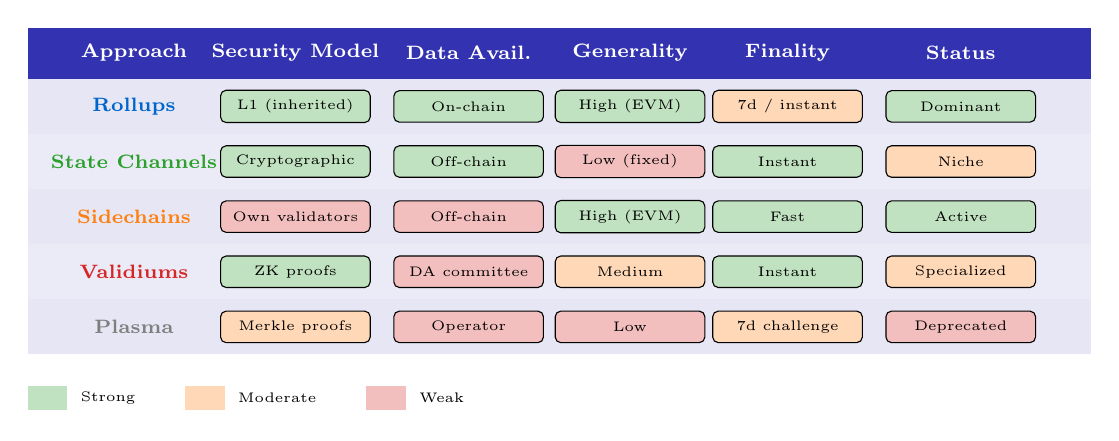
\begin{tikzpicture}[scale=1.0, every node/.style={font=\scriptsize}]
  % Header row background
  \fill[mlpurple] (0, 4.3) rectangle (13.5, 4.95);
  % Column header text
  \node[text=white,font=\scriptsize\bfseries,align=center] at (1.35, 4.63) {Approach};
  \node[text=white,font=\scriptsize\bfseries,align=center] at (3.40, 4.63) {Security Model};
  \node[text=white,font=\scriptsize\bfseries,align=center] at (5.60, 4.63) {Data Avail.};
  \node[text=white,font=\scriptsize\bfseries,align=center] at (7.65, 4.63) {Generality};
  \node[text=white,font=\scriptsize\bfseries,align=center] at (9.65, 4.63) {Finality};
  \node[text=white,font=\scriptsize\bfseries,align=center] at (11.85, 4.63) {Status};

  % Row colors: alternating
  \fill[mllavender4!60]  (0, 3.6) rectangle (13.5, 4.3);
  \fill[mllavender3!40]  (0, 2.9) rectangle (13.5, 3.6);
  \fill[mllavender4!60]  (0, 2.2) rectangle (13.5, 2.9);
  \fill[mllavender3!40]  (0, 1.5) rectangle (13.5, 2.2);
  \fill[mllavender4!60]  (0, 0.8) rectangle (13.5, 1.5);

  % Row 1: Rollups
  \node[align=center,font=\scriptsize\bfseries,text=mlblue] at (1.35, 3.95) {Rollups};
  \node[draw,fill=mlgreen!30,rounded corners=2pt,minimum width=1.9cm,minimum height=0.4cm,align=center,font=\tiny]
    at (3.40, 3.95) {L1 (inherited)};
  \node[draw,fill=mlgreen!30,rounded corners=2pt,minimum width=1.9cm,minimum height=0.4cm,align=center,font=\tiny]
    at (5.60, 3.95) {On-chain};
  \node[draw,fill=mlgreen!30,rounded corners=2pt,minimum width=1.9cm,minimum height=0.4cm,align=center,font=\tiny]
    at (7.65, 3.95) {High (EVM)};
  \node[draw,fill=mlorange!30,rounded corners=2pt,minimum width=1.9cm,minimum height=0.4cm,align=center,font=\tiny]
    at (9.65, 3.95) {7d / instant};
  \node[draw,fill=mlgreen!30,rounded corners=2pt,minimum width=1.9cm,minimum height=0.4cm,align=center,font=\tiny]
    at (11.85, 3.95) {Dominant};

  % Row 2: State Channels
  \node[align=center,font=\scriptsize\bfseries,text=mlgreen] at (1.35, 3.25) {State Channels};
  \node[draw,fill=mlgreen!30,rounded corners=2pt,minimum width=1.9cm,minimum height=0.4cm,align=center,font=\tiny]
    at (3.40, 3.25) {Cryptographic};
  \node[draw,fill=mlgreen!30,rounded corners=2pt,minimum width=1.9cm,minimum height=0.4cm,align=center,font=\tiny]
    at (5.60, 3.25) {Off-chain};
  \node[draw,fill=mlred!30,rounded corners=2pt,minimum width=1.9cm,minimum height=0.4cm,align=center,font=\tiny]
    at (7.65, 3.25) {Low (fixed)};
  \node[draw,fill=mlgreen!30,rounded corners=2pt,minimum width=1.9cm,minimum height=0.4cm,align=center,font=\tiny]
    at (9.65, 3.25) {Instant};
  \node[draw,fill=mlorange!30,rounded corners=2pt,minimum width=1.9cm,minimum height=0.4cm,align=center,font=\tiny]
    at (11.85, 3.25) {Niche};

  % Row 3: Sidechains
  \node[align=center,font=\scriptsize\bfseries,text=mlorange] at (1.35, 2.55) {Sidechains};
  \node[draw,fill=mlred!30,rounded corners=2pt,minimum width=1.9cm,minimum height=0.4cm,align=center,font=\tiny]
    at (3.40, 2.55) {Own validators};
  \node[draw,fill=mlred!30,rounded corners=2pt,minimum width=1.9cm,minimum height=0.4cm,align=center,font=\tiny]
    at (5.60, 2.55) {Off-chain};
  \node[draw,fill=mlgreen!30,rounded corners=2pt,minimum width=1.9cm,minimum height=0.4cm,align=center,font=\tiny]
    at (7.65, 2.55) {High (EVM)};
  \node[draw,fill=mlgreen!30,rounded corners=2pt,minimum width=1.9cm,minimum height=0.4cm,align=center,font=\tiny]
    at (9.65, 2.55) {Fast};
  \node[draw,fill=mlgreen!30,rounded corners=2pt,minimum width=1.9cm,minimum height=0.4cm,align=center,font=\tiny]
    at (11.85, 2.55) {Active};

  % Row 4: Validiums
  \node[align=center,font=\scriptsize\bfseries,text=mlred] at (1.35, 1.85) {Validiums};
  \node[draw,fill=mlgreen!30,rounded corners=2pt,minimum width=1.9cm,minimum height=0.4cm,align=center,font=\tiny]
    at (3.40, 1.85) {ZK proofs};
  \node[draw,fill=mlred!30,rounded corners=2pt,minimum width=1.9cm,minimum height=0.4cm,align=center,font=\tiny]
    at (5.60, 1.85) {DA committee};
  \node[draw,fill=mlorange!30,rounded corners=2pt,minimum width=1.9cm,minimum height=0.4cm,align=center,font=\tiny]
    at (7.65, 1.85) {Medium};
  \node[draw,fill=mlgreen!30,rounded corners=2pt,minimum width=1.9cm,minimum height=0.4cm,align=center,font=\tiny]
    at (9.65, 1.85) {Instant};
  \node[draw,fill=mlorange!30,rounded corners=2pt,minimum width=1.9cm,minimum height=0.4cm,align=center,font=\tiny]
    at (11.85, 1.85) {Specialized};

  % Row 5: Plasma
  \node[align=center,font=\scriptsize\bfseries,text=mlgray] at (1.35, 1.15) {Plasma};
  \node[draw,fill=mlorange!30,rounded corners=2pt,minimum width=1.9cm,minimum height=0.4cm,align=center,font=\tiny]
    at (3.40, 1.15) {Merkle proofs};
  \node[draw,fill=mlred!30,rounded corners=2pt,minimum width=1.9cm,minimum height=0.4cm,align=center,font=\tiny]
    at (5.60, 1.15) {Operator};
  \node[draw,fill=mlred!30,rounded corners=2pt,minimum width=1.9cm,minimum height=0.4cm,align=center,font=\tiny]
    at (7.65, 1.15) {Low};
  \node[draw,fill=mlorange!30,rounded corners=2pt,minimum width=1.9cm,minimum height=0.4cm,align=center,font=\tiny]
    at (9.65, 1.15) {7d challenge};
  \node[draw,fill=mlred!30,rounded corners=2pt,minimum width=1.9cm,minimum height=0.4cm,align=center,font=\tiny]
    at (11.85, 1.15) {Deprecated};

  % Legend
  \fill[mlgreen!30] (0.0, 0.1) rectangle (0.5, 0.4);
  \node[font=\tiny,right] at (0.55, 0.25) {Strong};
  \fill[mlorange!30] (2.0, 0.1) rectangle (2.5, 0.4);
  \node[font=\tiny,right] at (2.55, 0.25) {Moderate};
  \fill[mlred!30] (4.3, 0.1) rectangle (4.8, 0.4);
  \node[font=\tiny,right] at (4.85, 0.25) {Weak};
\end{tikzpicture}
\bottomnote{Rollups are the dominant L2 paradigm because they inherit L1 security while supporting general-purpose computation}
\end{frame}

% Frame 12: How Rollups Work (General)
\begin{frame}{How Rollups Work (General)}
\vspace{-1mm}
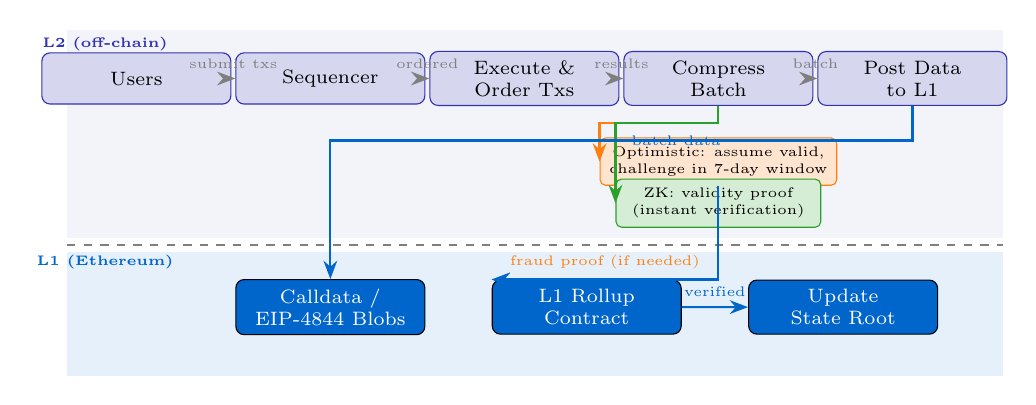
\begin{tikzpicture}[
  scale=0.88,
  every node/.style={font=\scriptsize},
  actor/.style={draw,rounded corners=3pt,minimum width=2.4cm,minimum height=0.65cm,
                align=center,fill=mllavender4,draw=mlpurple},
  l1box/.style={draw,rounded corners=3pt,minimum width=2.4cm,minimum height=0.65cm,
                align=center,fill=mlblue,text=white},
  arr/.style={-{Stealth},thick,mlgray},
  proofopt/.style={draw,rounded corners=2pt,fill=mlorange!20,draw=mlorange,
                   minimum width=2.6cm,minimum height=0.55cm,align=center,font=\tiny},
  proofzk/.style={draw,rounded corners=2pt,fill=mlgreen!20,draw=mlgreen,
                  minimum width=2.6cm,minimum height=0.55cm,align=center,font=\tiny},
]
  % L2 region label
  \fill[mllavender4!30] (0, 2.2) rectangle (13.5, 5.2);
  \node[font=\tiny\bfseries,text=mlpurple] at (0.55, 5.0) {L2 (off-chain)};

  % L1 region label
  \fill[mlblue!10] (0, 0.2) rectangle (13.5, 2.0);
  \node[font=\tiny\bfseries,text=mlblue] at (0.55, 1.85) {L1 (Ethereum)};

  % Dashed boundary
  \draw[dashed,thick,mlgray] (0, 2.1) -- (13.5, 2.1);

  % L2 actors
  \node[actor] (users)  at (1.0,  4.5) {Users};
  \node[actor] (seq)    at (3.8,  4.5) {Sequencer};
  \node[actor] (exec)   at (6.6,  4.5) {Execute \&\\Order Txs};
  \node[actor] (comp)   at (9.4,  4.5) {Compress\\Batch};
  \node[actor] (post)   at (12.2, 4.5) {Post Data\\to L1};

  % L2 flow
  \draw[arr] (users) -- (seq)   node[midway,above,font=\tiny] {submit txs};
  \draw[arr] (seq)   -- (exec)  node[midway,above,font=\tiny] {ordered};
  \draw[arr] (exec)  -- (comp)  node[midway,above,font=\tiny] {results};
  \draw[arr] (comp)  -- (post)  node[midway,above,font=\tiny] {batch};

  % Proof fork
  \node[proofopt] (opf) at (9.4, 3.3) {Optimistic: assume valid,\\challenge in 7-day window};
  \node[proofzk]  (zkf) at (9.4, 2.7) {ZK: validity proof\\(instant verification)};
  \draw[arr,mlorange] (comp.south) -- ++(0,-0.25) -| (opf.west);
  \draw[arr,mlgreen]  (comp.south) -- ++(0,-0.25) -| (zkf.west);

  % L1 components
  \node[l1box] (callda) at (3.8,  1.2) {Calldata /\\EIP-4844 Blobs};
  \node[l1box] (l1con)  at (7.5,  1.2) {L1 Rollup\\Contract};
  \node[l1box] (sroot)  at (11.2, 1.2) {Update\\State Root};

  % L2 -> L1 arrows
  \draw[arr,mlblue,thick] (post.south)  -- ++(0,-0.5) -| (callda.north)
    node[near start,right,font=\tiny,text=mlblue] {batch data};
  \draw[arr,mlblue,thick] (opf.south)   |- (l1con.north west)
    node[near end,above,font=\tiny,text=mlorange] {fraud proof (if needed)};
  \draw[arr,mlblue,thick] (zkf.south)   |- (l1con.north west);
  \draw[arr,mlblue,thick] (l1con) -- (sroot)
    node[midway,above,font=\tiny] {verified};
\end{tikzpicture}
\bottomnote{Both rollup types post transaction data to L1 -- the key difference is how correctness is proven: fraud proofs vs validity proofs}
\end{frame}

% Frame 13: Data Compression in Rollups
\begin{frame}{Data Compression in Rollups}
\begin{columns}[T]
\column{0.50\textwidth}
\begin{block}{How Rollups Compress Data}
\footnotesize
\begin{itemize}
  \item \textbf{Full L1 transaction}: \textasciitilde110 bytes
    \begin{itemize}\scriptsize
      \item Signature (65 bytes), nonce (3), gas (3), to (20), value (8), data (varies)
    \end{itemize}
  \item \textbf{Rollup compressed}: \textasciitilde12 bytes
    \begin{itemize}\scriptsize
      \item Address delta (4 bytes), nonce (2), amount (8)
    \end{itemize}
  \item \textbf{Compression ratio}: \textasciitilde10$\times$
  \item \textbf{Signature aggregation}: BLS signatures or ZK validity proofs eliminate per-tx signatures entirely
  \item \textbf{EIP-4844 blobs}: Separate cheaper data market vs calldata (\textasciitilde10$\times$ cheaper again)
\end{itemize}
\end{block}
\vspace{2mm}
\begin{block}{Cost Savings Calculation}
\footnotesize
\begin{tabular}{lrr}
\toprule
Scenario & 1{,}000 Txs & Cost (est.) \\
\midrule
L1 native & 1{,}000 txs & \$50{,}000 \\
Rollup (calldata) & 1 batch & \$500 \\
Rollup (blob) & 1 batch & \$50 \\
\bottomrule
\end{tabular}\\[2mm]
\textit{\scriptsize Savings: 100$\times$--1{,}000$\times$ depending on blob availability}
\end{block}
\column{0.50\textwidth}
\vspace{3mm}
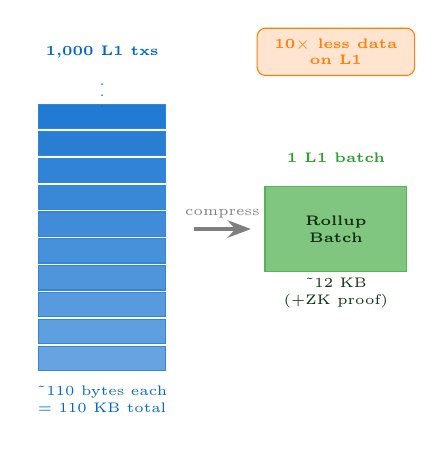
\begin{tikzpicture}[scale=0.9, every node/.style={font=\scriptsize}]
  % Left stack: 1000 L1 transactions (explicit rectangles, no \foreach)
  \fill[mlblue!60,draw=mlblue!80] (0, 0.00) rectangle (1.8, 0.34);
  \fill[mlblue!63,draw=mlblue!80] (0, 0.38) rectangle (1.8, 0.72);
  \fill[mlblue!66,draw=mlblue!80] (0, 0.76) rectangle (1.8, 1.10);
  \fill[mlblue!69,draw=mlblue!80] (0, 1.14) rectangle (1.8, 1.48);
  \fill[mlblue!72,draw=mlblue!80] (0, 1.52) rectangle (1.8, 1.86);
  \fill[mlblue!75,draw=mlblue!80] (0, 1.90) rectangle (1.8, 2.24);
  \fill[mlblue!78,draw=mlblue!80] (0, 2.28) rectangle (1.8, 2.62);
  \fill[mlblue!81,draw=mlblue!80] (0, 2.66) rectangle (1.8, 3.00);
  \fill[mlblue!84,draw=mlblue!80] (0, 3.04) rectangle (1.8, 3.38);
  \fill[mlblue!87,draw=mlblue!80] (0, 3.42) rectangle (1.8, 3.76);
  % Dots indicating more
  \node[font=\tiny,text=mlblue] at (0.9, 4.0) {$\vdots$};
  \node[font=\tiny\bfseries,text=mlblue,align=center] at (0.9, 4.5)
    {1{,}000 L1 txs};
  \node[font=\tiny,text=mlblue,align=center] at (0.9, -0.4)
    {\textasciitilde110 bytes each\\= 110 KB total};

  % Arrow
  \draw[-{Stealth},very thick,mlgray] (2.2, 2.0) -- (3.0, 2.0)
    node[midway,above,font=\tiny] {compress};

  % Right block: rollup batch
  \fill[mlgreen!60,draw=mlgreen!80] (3.2, 1.4) rectangle (5.2, 2.6);
  \node[align=center,font=\tiny\bfseries,text=mlgreen!30!black]
    at (4.2, 2.0) {Rollup\\Batch};
  \node[font=\tiny,text=mlgreen!30!black,align=center] at (4.2, 1.1)
    {\textasciitilde12 KB\\(+ZK proof)};
  \node[font=\tiny\bfseries,text=mlgreen,align=center] at (4.2, 3.0)
    {1 L1 batch};

  % Savings label
  \node[draw,fill=mlorange!20,draw=mlorange,rounded corners=3pt,
        minimum width=2.0cm,minimum height=0.6cm,align=center,font=\tiny\bfseries,
        text=mlorange] at (4.2, 4.5)
    {10$\times$ less data\\on L1};
\end{tikzpicture}
\end{columns}
\bottomnote{Data compression is the key economic advantage of rollups -- less data on L1 means lower costs per transaction}
\end{frame}

% Frame 14: Section 1 Summary
\begin{frame}{Section 1 Summary}
\vspace{2mm}
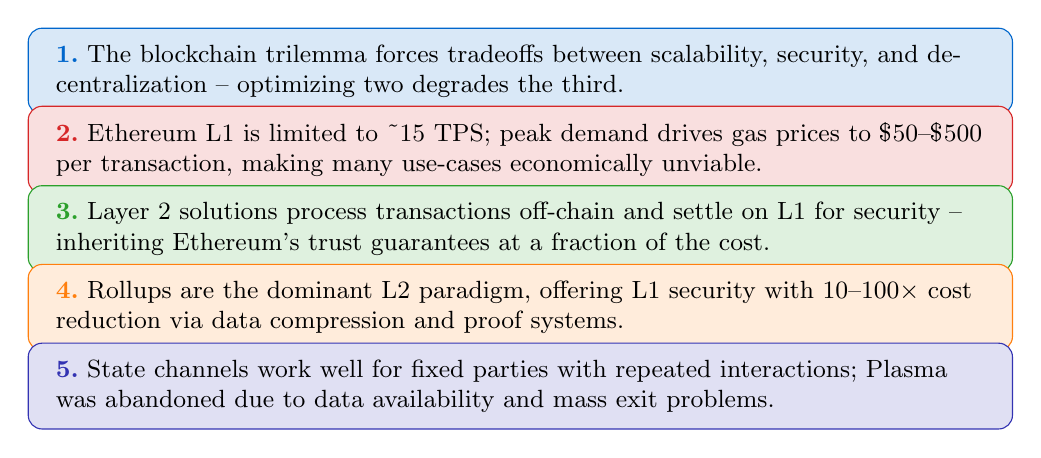
\begin{tikzpicture}[
  scale=1.0,
  every node/.style={font=\small},
  sumbox/.style={draw,rounded corners=5pt,minimum width=12.5cm,minimum height=0.85cm,
                 align=left,text width=11.8cm,inner sep=6pt},
]
  % Box 1
  \node[sumbox,fill=mlblue!15,draw=mlblue] (k1) at (6.5, 4.5) {%
    \textbf{\textcolor{mlblue}{1.}}~The blockchain trilemma forces tradeoffs between
    scalability, security, and decentralization -- optimizing two degrades the third.
  };
  % Box 2
  \node[sumbox,fill=mlred!15,draw=mlred] (k2) at (6.5, 3.5) {%
    \textbf{\textcolor{mlred}{2.}}~Ethereum L1 is limited to \textasciitilde15 TPS;
    peak demand drives gas prices to \$50--\$500 per transaction, making many use-cases economically unviable.
  };
  % Box 3
  \node[sumbox,fill=mlgreen!15,draw=mlgreen] (k3) at (6.5, 2.5) {%
    \textbf{\textcolor{mlgreen}{3.}}~Layer 2 solutions process transactions off-chain
    and settle on L1 for security -- inheriting Ethereum's trust guarantees at a fraction of the cost.
  };
  % Box 4
  \node[sumbox,fill=mlorange!15,draw=mlorange] (k4) at (6.5, 1.5) {%
    \textbf{\textcolor{mlorange}{4.}}~Rollups are the dominant L2 paradigm, offering
    L1 security with 10--100$\times$ cost reduction via data compression and proof systems.
  };
  % Box 5
  \node[sumbox,fill=mlpurple!15,draw=mlpurple] (k5) at (6.5, 0.5) {%
    \textbf{\textcolor{mlpurple}{5.}}~State channels work well for fixed parties with repeated
    interactions; Plasma was abandoned due to data availability and mass exit problems.
  };
\end{tikzpicture}
\bottomnote{Section 1 complete -- next: Optimistic Rollups (Arbitrum, Optimism) and fraud proof mechanisms}
\end{frame}

%% ============================================================
%% SECTION 2: Optimistic Rollups
%% ============================================================
\section{Optimistic Rollups}

% Frame 15: Section 2 Divider
\begin{frame}{}
\vspace{10mm}
\begin{beamercolorbox}[sep=12pt,center,rounded=true,shadow=true]{palette quaternary}
{\Large\bfseries Section 2: Optimistic Rollups}\\[6pt]
{\normalsize Fraud proofs, challenge periods, and the optimistic approach to scaling}
\end{beamercolorbox}
\vspace{6mm}
\begin{columns}[T]
\begin{column}{0.48\textwidth}
\begin{block}{What You Will Learn}
\begin{itemize}\setlength\itemsep{3pt}
  \item[\small$\checkmark$] \small How optimistic rollups assume validity and verify via fraud proofs
  \item[\small$\checkmark$] \small Sequencer role, centralization risks, and decentralization roadmaps
  \item[\small$\checkmark$] \small Challenge period mechanics and dispute resolution
  \item[\small$\checkmark$] \small Arbitrum, Optimism, and Base architecture comparisons
\end{itemize}
\end{block}
\end{column}
\begin{column}{0.48\textwidth}
\begin{block}{Frames in This Section}
\begin{itemize}\setlength\itemsep{3pt}
  \item[\small$\bullet$] \small Frame 16: Optimistic Rollup Architecture
  \item[\small$\bullet$] \small Frame 17: Fraud Proof Mechanism
  \item[\small$\bullet$] \small Frame 18: Fraud Proof Challenge (Code)
  \item[\small$\bullet$] \small Frames 19--24: Sequencer, Arbitrum, Optimism, Base, Fees, Comparison
  \item[\small$\bullet$] \small Frame 25: Section Summary
\end{itemize}
\end{block}
\end{column}
\end{columns}
\bottomnote{Section 2 of 5 -- Optimistic Rollups: trust but verify approach to scaling}
\end{frame}

% Frame 16: Optimistic Rollup Architecture
\begin{frame}{Optimistic Rollup Architecture}
\vspace{-1mm}
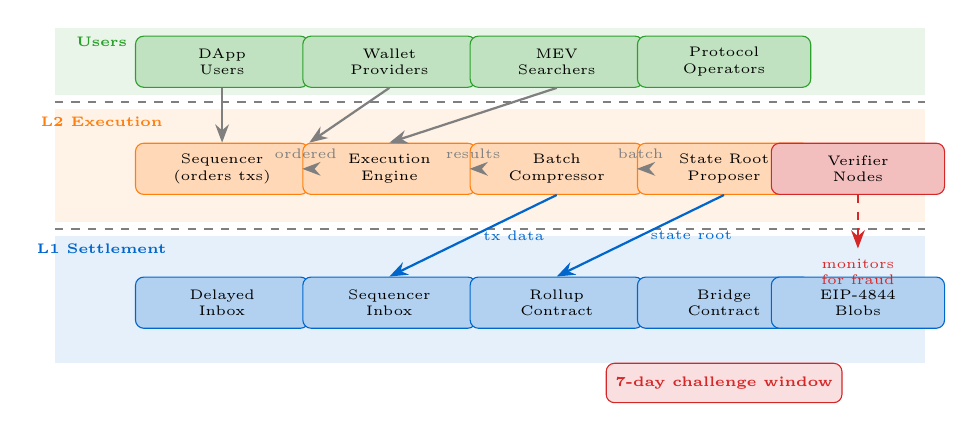
\begin{tikzpicture}[
  scale=0.85,
  every node/.style={font=\scriptsize},
  l2layer/.style={draw,rounded corners=4pt,minimum width=12.5cm,minimum height=1.5cm,
                  align=center},
  l2comp/.style={draw,rounded corners=3pt,minimum width=2.2cm,minimum height=0.65cm,
                 align=center,font=\tiny},
  arr/.style={-{Stealth},thick,mlgray},
]
  % User layer (top)
  \fill[mlgreen!10] (0.0, 4.6) rectangle (13.0, 5.6);
  \node[font=\tiny\bfseries,text=mlgreen] at (0.7, 5.4) {Users};
  \node[l2comp,fill=mlgreen!30,draw=mlgreen] (u1) at (2.5, 5.1) {DApp\\Users};
  \node[l2comp,fill=mlgreen!30,draw=mlgreen] (u2) at (5.0, 5.1) {Wallet\\Providers};
  \node[l2comp,fill=mlgreen!30,draw=mlgreen] (u3) at (7.5, 5.1) {MEV\\Searchers};
  \node[l2comp,fill=mlgreen!30,draw=mlgreen] (u4) at (10.0, 5.1) {Protocol\\Operators};

  % L2 execution layer (middle)
  \fill[mlorange!10] (0.0, 2.7) rectangle (13.0, 4.4);
  \node[font=\tiny\bfseries,text=mlorange] at (0.7, 4.2) {L2 Execution};
  \node[l2comp,fill=mlorange!30,draw=mlorange] (seq) at (2.5, 3.5) {Sequencer\\(orders txs)};
  \node[l2comp,fill=mlorange!30,draw=mlorange] (exe) at (5.0, 3.5) {Execution\\Engine};
  \node[l2comp,fill=mlorange!30,draw=mlorange] (bat) at (7.5, 3.5) {Batch\\Compressor};
  \node[l2comp,fill=mlorange!30,draw=mlorange] (pro) at (10.0, 3.5) {State Root\\Proposer};
  \node[l2comp,fill=mlred!30,draw=mlred] (ver) at (12.0, 3.5) {Verifier\\Nodes};

  % L1 settlement layer (bottom)
  \fill[mlblue!10] (0.0, 0.6) rectangle (13.0, 2.5);
  \node[font=\tiny\bfseries,text=mlblue] at (0.7, 2.3) {L1 Settlement};
  \node[l2comp,fill=mlblue!30,draw=mlblue] (inbox) at (2.5, 1.5) {Delayed\\Inbox};
  \node[l2comp,fill=mlblue!30,draw=mlblue] (seqin) at (5.0, 1.5) {Sequencer\\Inbox};
  \node[l2comp,fill=mlblue!30,draw=mlblue] (roll) at (7.5, 1.5) {Rollup\\Contract};
  \node[l2comp,fill=mlblue!30,draw=mlblue] (bridge) at (10.0, 1.5) {Bridge\\Contract};
  \node[l2comp,fill=mlblue!30,draw=mlblue] (blob) at (12.0, 1.5) {EIP-4844\\Blobs};

  % Dashed boundaries
  \draw[dashed,thick,mlgray] (0.0, 4.5) -- (13.0, 4.5);
  \draw[dashed,thick,mlgray] (0.0, 2.6) -- (13.0, 2.6);

  % User -> L2 arrows
  \draw[arr] (u1.south) -- (seq.north);
  \draw[arr] (u2.south) -- (seq.north east);
  \draw[arr] (u3.south) -- (exe.north);

  % L2 internal flow
  \draw[arr] (seq) -- (exe) node[midway,above,font=\tiny] {ordered};
  \draw[arr] (exe) -- (bat) node[midway,above,font=\tiny] {results};
  \draw[arr] (bat) -- (pro) node[midway,above,font=\tiny] {batch};

  % Verifier watching
  \draw[-{Stealth},dashed,mlred,thick] (ver.south) -- ++(0,-0.8)
    node[below,font=\tiny,text=mlred,align=center] {monitors\\for fraud};

  % L2 -> L1 arrows
  \draw[arr,mlblue] (bat.south) -- (seqin.north)
    node[midway,right,font=\tiny,text=mlblue] {tx data};
  \draw[arr,mlblue] (pro.south) -- (roll.north)
    node[midway,right,font=\tiny,text=mlblue] {state root};

  % Challenge annotation
  \node[draw,fill=mlred!15,draw=mlred,rounded corners=3pt,
        minimum width=2.8cm,minimum height=0.5cm,align=center,font=\tiny\bfseries,
        text=mlred] at (10.0, 0.3) {7-day challenge window};
\end{tikzpicture}
\bottomnote{Optimistic rollups assume all batches are valid -- anyone can challenge with a fraud proof within the 7-day window}
\end{frame}

% Frame 17: Fraud Proof Mechanism
\begin{frame}{Fraud Proof Mechanism}
\vspace{-2mm}
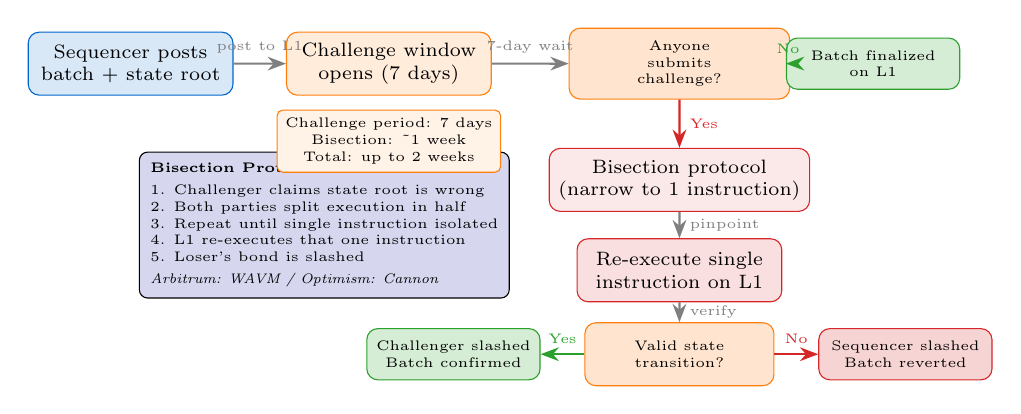
\begin{tikzpicture}[
  scale=0.82,
  every node/.style={font=\scriptsize},
  fpbox/.style={draw,rounded corners=4pt,minimum width=2.6cm,minimum height=0.8cm,
                align=center,fill=mllavender4,draw=mlpurple},
  decbox/.style={draw,rounded corners=4pt,minimum width=2.4cm,minimum height=0.7cm,
                 align=center,fill=mlorange!20,draw=mlorange,font=\tiny},
  okbox/.style={draw,rounded corners=4pt,minimum width=2.2cm,minimum height=0.65cm,
                align=center,fill=mlgreen!20,draw=mlgreen,font=\tiny},
  failbox/.style={draw,rounded corners=4pt,minimum width=2.2cm,minimum height=0.65cm,
                  align=center,fill=mlred!20,draw=mlred,font=\tiny},
  arr/.style={-{Stealth},thick,mlgray},
]
  % Step 1: Sequencer posts batch
  \node[fpbox,fill=mlblue!15,draw=mlblue] (s1) at (1.5, 5.0)
    {Sequencer posts\\batch + state root};

  % Step 2: Challenge window opens
  \node[fpbox,fill=mlorange!15,draw=mlorange] (s2) at (5.5, 5.0)
    {Challenge window\\opens (7 days)};

  % Step 3: Decision -- anyone challenges?
  \node[decbox,minimum width=2.8cm,minimum height=0.9cm] (dec) at (10.0, 5.0)
    {Anyone\\submits\\challenge?};

  % No challenge path
  \node[okbox] (ok) at (13.0, 5.0) {Batch finalized\\on L1};

  % Yes challenge path -- bisection
  \node[fpbox,fill=mlred!10,draw=mlred] (bis) at (10.0, 3.2)
    {Bisection protocol\\(narrow to 1 instruction)};

  % Re-execute on L1
  \node[fpbox,fill=mlred!15,draw=mlred] (reexec) at (10.0, 1.8)
    {Re-execute single\\instruction on L1};

  % Final decision
  \node[decbox,minimum width=2.4cm,minimum height=0.8cm] (vdec) at (10.0, 0.5)
    {Valid state\\transition?};

  % Outcomes
  \node[okbox] (valid) at (6.5, 0.5) {Challenger slashed\\Batch confirmed};
  \node[failbox] (invalid) at (13.5, 0.5) {Sequencer slashed\\Batch reverted};

  % Arrows
  \draw[arr] (s1) -- (s2) node[midway,above,font=\tiny] {post to L1};
  \draw[arr] (s2) -- (dec) node[midway,above,font=\tiny] {7-day wait};
  \draw[arr,mlgreen] (dec) -- (ok) node[midway,above,font=\tiny,text=mlgreen] {No};
  \draw[arr,mlred] (dec) -- (bis) node[midway,right,font=\tiny,text=mlred] {Yes};
  \draw[arr] (bis) -- (reexec) node[midway,right,font=\tiny] {pinpoint};
  \draw[arr] (reexec) -- (vdec) node[midway,right,font=\tiny] {verify};
  \draw[arr,mlgreen] (vdec) -- (valid) node[midway,above,font=\tiny,text=mlgreen] {Yes};
  \draw[arr,mlred] (vdec) -- (invalid) node[midway,above,font=\tiny,text=mlred] {No};

  % Annotation: bisection detail
  \node[draw,fill=mllavender4,rounded corners=3pt,
        minimum width=4.5cm,align=left,font=\tiny,inner sep=4pt]
    at (4.5, 2.5) {%
      \textbf{Bisection Protocol:}\\[2pt]
      1. Challenger claims state root is wrong\\
      2. Both parties split execution in half\\
      3. Repeat until single instruction isolated\\
      4. L1 re-executes that one instruction\\
      5. Loser's bond is slashed\\[2pt]
      \textit{Arbitrum: WAVM / Optimism: Cannon}
    };

  % Time annotation
  \node[draw,fill=mlorange!10,draw=mlorange,rounded corners=2pt,
        align=center,font=\tiny,inner sep=3pt] at (5.5, 3.8)
    {Challenge period: 7 days\\Bisection: \textasciitilde1 week\\Total: up to 2 weeks};
\end{tikzpicture}
\bottomnote{Fraud proofs need only 1 honest verifier to catch cheating -- the bisection protocol narrows the dispute to a single instruction}
\end{frame}

% Frame 18: Fraud Proof Challenge [FRAGILE] -- CODE FRAME
\begin{frame}[fragile]{Fraud Proof Challenge}
\begin{columns}[T]
\column{0.50\textwidth}
\vspace{1mm}
\begin{lstlisting}[language=Solidity,caption={Simplified Fraud Proof}]
// Simplified Fraud Proof
contract OptimisticRollup {
    uint256 public challengePeriod
        = 7 days;
    mapping(bytes32 => uint256)
        public stateRoots;

    function submitBatch(
        bytes32 stateRoot,
        bytes calldata txData
    ) external onlySequencer {
        stateRoots[stateRoot] =
            block.timestamp;
        emit BatchSubmitted(
            stateRoot, txData);
    }

    function challengeBatch(
        bytes32 stateRoot,
        bytes calldata proof
    ) external {
        require(block.timestamp <
            stateRoots[stateRoot]
            + challengePeriod,
            "Challenge period over");
        require(verifyFraud(proof),
            "Invalid proof");
        delete stateRoots[stateRoot];
        // Slash sequencer bond
    }
}
\end{lstlisting}
\column{0.50\textwidth}
\vspace{2mm}
\begin{block}{Contract Analysis}
\footnotesize
\begin{itemize}
  \item \textbf{submitBatch}: Sequencer posts a new state root along with compressed transaction data
  \item \textbf{challengePeriod}: 7-day window during which anyone can dispute
  \item \textbf{challengeBatch}: Verifier submits a fraud proof; if valid, the batch is deleted and sequencer bond is slashed
  \item \textbf{Key insight}: Only the \textit{challenge path} is expensive -- the happy path costs minimal gas
\end{itemize}
\end{block}
\vspace{2mm}
\begin{block}{Security Assumptions}
\footnotesize
\begin{itemize}
  \item Requires at least \textbf{1 honest verifier} monitoring the chain
  \item Verifier must have enough time to submit proof (7 days)
  \item L1 must remain censorship-resistant for the proof to land
  \item Sequencer bond must exceed potential gains from fraud
\end{itemize}
\end{block}
\vspace{2mm}
\begin{alertblock}{Trust Model}
\footnotesize
``Optimistic'' = assume honest unless proven otherwise. Security is 1-of-N: only one honest watcher needed.
\end{alertblock}
\end{columns}
\bottomnote{Optimistic rollups only invoke the expensive fraud proof path when cheating is detected -- the happy path is cheap}
\end{frame}

% Frame 19: The Sequencer Role
\begin{frame}{The Sequencer Role}
\vspace{-1mm}
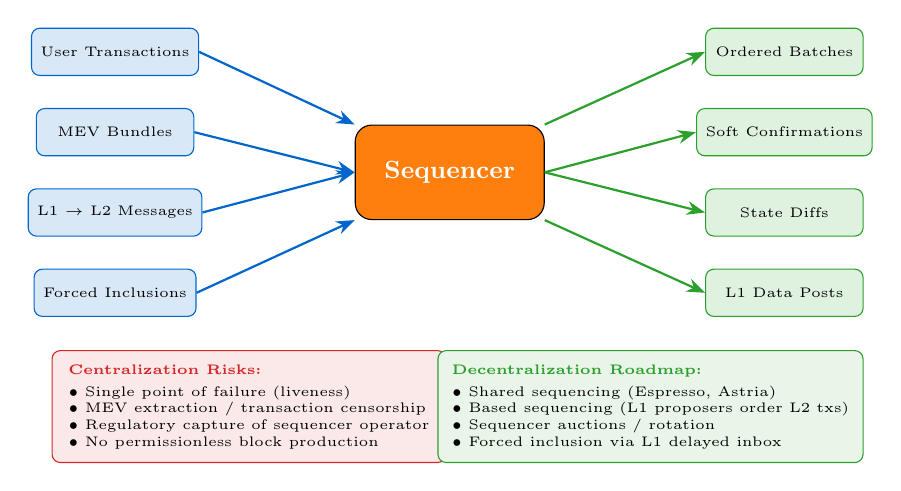
\begin{tikzpicture}[
  scale=0.85,
  every node/.style={font=\scriptsize},
  seqhub/.style={draw,rounded corners=6pt,fill=mlorange,text=white,
                 minimum width=2.4cm,minimum height=1.2cm,align=center,font=\small\bfseries},
  innode/.style={draw,rounded corners=3pt,fill=mlblue!15,draw=mlblue,
                 minimum width=2.0cm,minimum height=0.6cm,align=center,font=\tiny},
  outnode/.style={draw,rounded corners=3pt,fill=mlgreen!15,draw=mlgreen,
                  minimum width=2.0cm,minimum height=0.6cm,align=center,font=\tiny},
  arr/.style={-{Stealth},thick},
]
  % Central sequencer
  \node[seqhub] (seq) at (6.5, 3.0) {Sequencer};

  % Incoming nodes (left)
  \node[innode] (tx1) at (1.5, 4.8) {User Transactions};
  \node[innode] (tx2) at (1.5, 3.6) {MEV Bundles};
  \node[innode] (tx3) at (1.5, 2.4) {L1 $\to$ L2 Messages};
  \node[innode] (tx4) at (1.5, 1.2) {Forced Inclusions};

  % Outgoing nodes (right)
  \node[outnode] (out1) at (11.5, 4.8) {Ordered Batches};
  \node[outnode] (out2) at (11.5, 3.6) {Soft Confirmations};
  \node[outnode] (out3) at (11.5, 2.4) {State Diffs};
  \node[outnode] (out4) at (11.5, 1.2) {L1 Data Posts};

  % Incoming arrows
  \draw[arr,mlblue] (tx1.east) -- (seq.north west);
  \draw[arr,mlblue] (tx2.east) -- (seq.west);
  \draw[arr,mlblue] (tx3.east) -- (seq.west);
  \draw[arr,mlblue] (tx4.east) -- (seq.south west);

  % Outgoing arrows
  \draw[arr,mlgreen] (seq.north east) -- (out1.west);
  \draw[arr,mlgreen] (seq.east) -- (out2.west);
  \draw[arr,mlgreen] (seq.east) -- (out3.west);
  \draw[arr,mlgreen] (seq.south east) -- (out4.west);

  % Centralization concerns (bottom left)
  \node[draw,fill=mlred!10,draw=mlred,rounded corners=3pt,
        minimum width=5.0cm,align=left,font=\tiny,inner sep=5pt]
    at (3.5, -0.5) {%
      \textbf{\textcolor{mlred}{Centralization Risks:}}\\[2pt]
      $\bullet$ Single point of failure (liveness)\\
      $\bullet$ MEV extraction / transaction censorship\\
      $\bullet$ Regulatory capture of sequencer operator\\
      $\bullet$ No permissionless block production
    };

  % Decentralization roadmap (bottom right)
  \node[draw,fill=mlgreen!10,draw=mlgreen,rounded corners=3pt,
        minimum width=5.0cm,align=left,font=\tiny,inner sep=5pt]
    at (9.5, -0.5) {%
      \textbf{\textcolor{mlgreen}{Decentralization Roadmap:}}\\[2pt]
      $\bullet$ Shared sequencing (Espresso, Astria)\\
      $\bullet$ Based sequencing (L1 proposers order L2 txs)\\
      $\bullet$ Sequencer auctions / rotation\\
      $\bullet$ Forced inclusion via L1 delayed inbox
    };
\end{tikzpicture}
\bottomnote{Today most optimistic rollups run a single centralized sequencer -- decentralization is the next major milestone}
\end{frame}

% Frame 20: Arbitrum Deep Dive
\begin{frame}{Arbitrum Deep Dive}
\begin{columns}[T]
\column{0.48\textwidth}
\begin{block}{Arbitrum Ecosystem}
\footnotesize
\begin{itemize}
  \item \textbf{Arbitrum One}: Flagship optimistic rollup; largest L2 by TVL
  \item \textbf{Arbitrum Nova}: AnyTrust chain for gaming/social (off-chain DA via committee)
  \item \textbf{Arbitrum Orbit}: Framework for launching custom L3 chains
  \item \textbf{Nitro}: Current execution engine -- compiles Geth to WASM for fraud proofs
  \item \textbf{Bold}: New permissionless dispute protocol (replaces single-challenger model)
\end{itemize}
\end{block}
\vspace{2mm}
\begin{block}{Key Metrics}
\footnotesize
\begin{tabular}{ll}
\toprule
Metric & Value \\
\midrule
Peak TPS & \textasciitilde4{,}000 \\
Avg Fee & \$0.01--\$0.10 \\
TVL & \textasciitilde\$18B (2024 peak) \\
Challenge Period & 7 days \\
Token & ARB (governance) \\
\bottomrule
\end{tabular}
\end{block}
\column{0.52\textwidth}
\vspace{1mm}
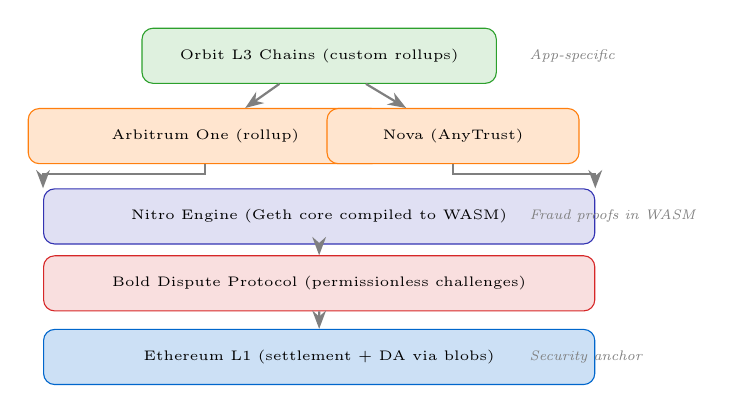
\begin{tikzpicture}[
  scale=0.85,
  every node/.style={font=\scriptsize},
  arbbox/.style={draw,rounded corners=4pt,minimum width=4.5cm,minimum height=0.7cm,
                 align=center,font=\tiny},
  arr/.style={-{Stealth},thick,mlgray},
]
  % L3 layer
  \node[arbbox,fill=mlgreen!15,draw=mlgreen] (orbit) at (3.5, 5.2)
    {Orbit L3 Chains (custom rollups)};

  % L2 layer
  \node[arbbox,fill=mlorange!20,draw=mlorange] (one) at (1.8, 4.0)
    {Arbitrum One (rollup)};
  \node[arbbox,fill=mlorange!20,draw=mlorange,minimum width=3.2cm] (nova) at (5.5, 4.0)
    {Nova (AnyTrust)};

  % Execution
  \node[arbbox,fill=mlpurple!15,draw=mlpurple,minimum width=7.0cm] (nitro) at (3.5, 2.8)
    {Nitro Engine (Geth core compiled to WASM)};

  % Dispute
  \node[arbbox,fill=mlred!15,draw=mlred,minimum width=7.0cm] (bold) at (3.5, 1.8)
    {Bold Dispute Protocol (permissionless challenges)};

  % L1 settlement
  \node[arbbox,fill=mlblue!20,draw=mlblue,minimum width=7.0cm] (l1) at (3.5, 0.7)
    {Ethereum L1 (settlement + DA via blobs)};

  % Arrows
  \draw[arr] (orbit) -- (one);
  \draw[arr] (orbit) -- (nova);
  \draw[arr] (one.south) -- ++(0,-0.15) -| (nitro.north west);
  \draw[arr] (nova.south) -- ++(0,-0.15) -| (nitro.north east);
  \draw[arr] (nitro) -- (bold);
  \draw[arr] (bold) -- (l1);

  % Labels
  \node[font=\tiny\itshape,text=mlgray,right] at (6.5, 5.2) {App-specific};
  \node[font=\tiny\itshape,text=mlgray,right] at (6.5, 2.8) {Fraud proofs in WASM};
  \node[font=\tiny\itshape,text=mlgray,right] at (6.5, 0.7) {Security anchor};
\end{tikzpicture}
\end{columns}
\bottomnote{Arbitrum One is the largest L2 by TVL -- Nitro compiles Geth to WASM so fraud proofs re-execute exact EVM logic}
\end{frame}

% Frame 21: Optimism & the OP Stack
\begin{frame}{Optimism \& the OP Stack}
\begin{columns}[T]
\column{0.48\textwidth}
\begin{block}{Optimism Ecosystem}
\footnotesize
\begin{itemize}
  \item \textbf{OP Mainnet}: Original optimistic rollup; second-largest by ecosystem
  \item \textbf{OP Stack}: Open-source modular rollup framework -- the ``Linux of rollups''
  \item \textbf{Superchain}: Vision for interconnected OP Stack chains sharing security and messaging
  \item \textbf{Fault Proofs}: Cannon/op-program -- permissionless fault proof system (live 2024)
  \item \textbf{Governance}: OP token + bicameral system (Token House + Citizens' House)
\end{itemize}
\end{block}
\vspace{2mm}
\begin{block}{OP Stack Adopters}
\footnotesize
\begin{itemize}
  \item \textbf{Base} (Coinbase) -- largest OP Stack chain
  \item \textbf{Zora} -- NFT-focused L2
  \item \textbf{Mode} -- DeFi-focused L2
  \item \textbf{World Chain} (Worldcoin) -- identity L2
  \item \textbf{20+ chains} deployed or announced
\end{itemize}
\end{block}
\column{0.52\textwidth}
\vspace{1mm}
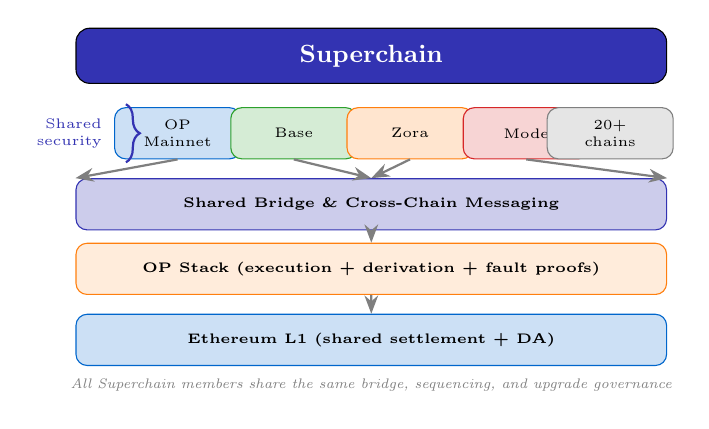
\begin{tikzpicture}[
  scale=0.82,
  every node/.style={font=\scriptsize},
  scbox/.style={draw,rounded corners=4pt,minimum width=1.6cm,minimum height=0.65cm,
                align=center,font=\tiny},
  arr/.style={-{Stealth},thick,mlgray},
]
  % Superchain label
  \node[draw,fill=mlpurple,text=white,rounded corners=5pt,
        minimum width=7.5cm,minimum height=0.7cm,align=center,font=\small\bfseries]
    (super) at (3.5, 5.5) {Superchain};

  % Individual chains
  \node[scbox,fill=mlblue!20,draw=mlblue] (op) at (0.5, 4.3) {OP\\Mainnet};
  \node[scbox,fill=mlgreen!20,draw=mlgreen] (base) at (2.3, 4.3) {Base};
  \node[scbox,fill=mlorange!20,draw=mlorange] (zora) at (4.1, 4.3) {Zora};
  \node[scbox,fill=mlred!20,draw=mlred] (mode) at (5.9, 4.3) {Mode};
  \node[scbox,fill=mlgray!20,draw=mlgray] (more) at (7.2, 4.3) {20+\\chains};

  % Shared layer
  \node[draw,fill=mllavender3,draw=mlpurple,rounded corners=4pt,
        minimum width=7.5cm,minimum height=0.65cm,align=center,font=\tiny\bfseries]
    (shared) at (3.5, 3.2) {Shared Bridge \& Cross-Chain Messaging};

  % OP Stack
  \node[draw,fill=mlorange!15,draw=mlorange,rounded corners=4pt,
        minimum width=7.5cm,minimum height=0.65cm,align=center,font=\tiny\bfseries]
    (stack) at (3.5, 2.2) {OP Stack (execution + derivation + fault proofs)};

  % L1
  \node[draw,fill=mlblue!20,draw=mlblue,rounded corners=4pt,
        minimum width=7.5cm,minimum height=0.65cm,align=center,font=\tiny\bfseries]
    (l1) at (3.5, 1.1) {Ethereum L1 (shared settlement + DA)};

  % Arrows from chains to shared
  \draw[arr] (op.south) -- (shared.north west);
  \draw[arr] (base.south) -- (shared.north);
  \draw[arr] (zora.south) -- (shared.north);
  \draw[arr] (mode.south) -- (shared.north east);

  % Shared -> Stack -> L1
  \draw[arr] (shared) -- (stack);
  \draw[arr] (stack) -- (l1);

  % Superchain to chains
  \draw[decorate,decoration={brace,amplitude=5pt,mirror},mlpurple,thick]
    (-0.3, 3.85) -- (-0.3, 4.75)
    node[midway,left=5pt,font=\tiny,text=mlpurple,align=right] {Shared\\security};

  % Cross-chain label
  \node[font=\tiny\itshape,text=mlgray] at (3.5, 0.4)
    {All Superchain members share the same bridge, sequencing, and upgrade governance};
\end{tikzpicture}
\end{columns}
\bottomnote{The OP Stack enables a ``Superchain'' of interoperable rollups -- Base, Zora, Mode, and 20+ chains share security}
\end{frame}

% Frame 22: Base & Coinbase L2
\begin{frame}{Base \& Coinbase L2}
\begin{columns}[T]
\column{0.48\textwidth}
\begin{block}{Base Overview}
\footnotesize
\begin{itemize}
  \item \textbf{Built on}: OP Stack (Optimism's modular framework)
  \item \textbf{Operator}: Coinbase -- leverages 110M+ verified users
  \item \textbf{No native token}: Revenue from sequencer fees; no token governance
  \item \textbf{Mission}: Bring the next 1 billion users on-chain
  \item \textbf{Launched}: August 2023
\end{itemize}
\end{block}
\vspace{2mm}
\begin{block}{Key Metrics}
\footnotesize
\begin{tabular}{ll}
\toprule
Metric & Value \\
\midrule
Daily Active Addresses & 2M+ (2024 peak) \\
Avg Fee & \$0.001--\$0.01 \\
TVL & \textasciitilde\$8B (2024 peak) \\
Sequencer & Coinbase (centralized) \\
Superchain member & Yes \\
\bottomrule
\end{tabular}
\end{block}
\vspace{2mm}
\begin{alertblock}{No-Token Model}
\footnotesize
Base has no native token. Coinbase earns revenue from sequencer fees and contributes to OP Collective governance via OP tokens.
\end{alertblock}
\column{0.52\textwidth}
\vspace{1mm}
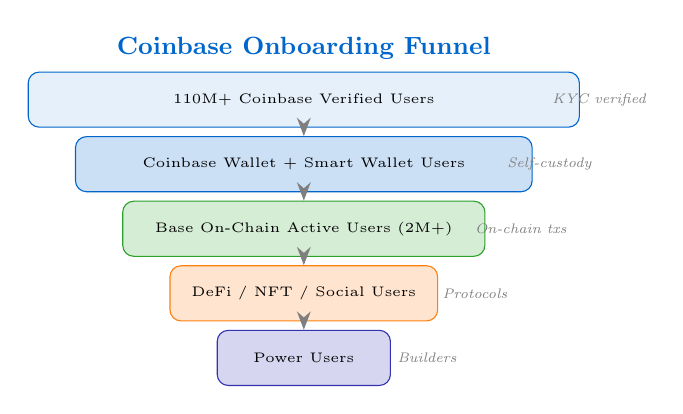
\begin{tikzpicture}[
  scale=0.82,
  every node/.style={font=\scriptsize},
  funnelbox/.style={draw,rounded corners=4pt,align=center,font=\tiny,
                    minimum height=0.7cm},
  arr/.style={-{Stealth},thick,mlgray},
]
  % Title
  \node[font=\small\bfseries,text=mlblue] at (3.5, 5.5) {Coinbase Onboarding Funnel};

  % Funnel layers (widest at top, narrowest at bottom)
  \node[funnelbox,fill=mlblue!10,draw=mlblue,minimum width=7.0cm]
    (f1) at (3.5, 4.7) {110M+ Coinbase Verified Users};
  \node[funnelbox,fill=mlblue!20,draw=mlblue,minimum width=5.8cm]
    (f2) at (3.5, 3.7) {Coinbase Wallet + Smart Wallet Users};
  \node[funnelbox,fill=mlgreen!20,draw=mlgreen,minimum width=4.6cm]
    (f3) at (3.5, 2.7) {Base On-Chain Active Users (2M+)};
  \node[funnelbox,fill=mlorange!20,draw=mlorange,minimum width=3.4cm]
    (f4) at (3.5, 1.7) {DeFi / NFT / Social Users};
  \node[funnelbox,fill=mlpurple!20,draw=mlpurple,minimum width=2.2cm]
    (f5) at (3.5, 0.7) {Power Users};

  % Arrows
  \draw[arr] (f1) -- (f2);
  \draw[arr] (f2) -- (f3);
  \draw[arr] (f3) -- (f4);
  \draw[arr] (f4) -- (f5);

  % Annotations on right
  \node[font=\tiny\itshape,text=mlgray,right] at (7.2, 4.7) {KYC verified};
  \node[font=\tiny\itshape,text=mlgray,right] at (6.5, 3.7) {Self-custody};
  \node[font=\tiny\itshape,text=mlgray,right] at (6.0, 2.7) {On-chain txs};
  \node[font=\tiny\itshape,text=mlgray,right] at (5.5, 1.7) {Protocols};
  \node[font=\tiny\itshape,text=mlgray,right] at (4.8, 0.7) {Builders};
\end{tikzpicture}
\end{columns}
\bottomnote{Base leverages Coinbase's 110M+ user base as the primary on-ramp to Ethereum L2 -- no native token, pure utility}
\end{frame}

% Frame 23: Optimistic Rollup Fee Structure
\begin{frame}{Optimistic Rollup Fee Structure}
\vspace{-1mm}
\begin{columns}[T]
\column{0.48\textwidth}
\begin{block}{Fee Decomposition}
\footnotesize
\textbf{Total Fee} = L1 Data Fee + L2 Execution Fee
\begin{itemize}
  \item \textbf{L1 Data Fee} (dominant cost): Posting compressed transaction data to Ethereum
    \begin{itemize}\scriptsize
      \item Pre-4844: via calldata (\textasciitilde16 gas/byte)
      \item Post-4844: via blobs (\textasciitilde1 gas/byte equivalent)
    \end{itemize}
  \item \textbf{L2 Execution Fee}: Gas for L2 computation (very cheap)
  \item \textbf{EIP-4844 impact}: 10--100$\times$ reduction in L1 data costs
\end{itemize}
\end{block}
\vspace{2mm}
\begin{block}{Fee Examples (2024 averages)}
\footnotesize
\begin{tabular}{lrr}
\toprule
Operation & Pre-4844 & Post-4844 \\
\midrule
ETH transfer & \$0.10 & \$0.001 \\
Token swap & \$0.30 & \$0.005 \\
NFT mint & \$0.50 & \$0.01 \\
Complex DeFi & \$1.00 & \$0.02 \\
\bottomrule
\end{tabular}
\end{block}
\column{0.52\textwidth}
\vspace{1mm}
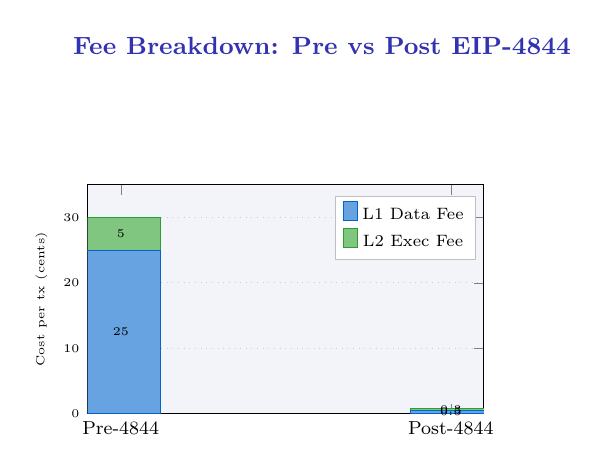
\begin{tikzpicture}[scale=0.85, every node/.style={font=\scriptsize}]
  % Fee breakdown diagram
  \node[font=\small\bfseries,text=mlpurple] at (3.5, 5.5) {Fee Breakdown: Pre vs Post EIP-4844};

  \begin{axis}[
    at={(0.0cm, 0.0cm)},
    width=7.5cm, height=5.0cm,
    ybar stacked,
    bar width=1.2cm,
    symbolic x coords={Pre-4844,Post-4844},
    xtick=data,
    xticklabel style={font=\footnotesize},
    yticklabel style={font=\tiny},
    ylabel={\tiny Cost per tx (cents)},
    ylabel style={font=\tiny},
    ymin=0, ymax=35,
    ymajorgrids=true,
    grid style={dotted,mlgray!40},
    axis background/.style={fill=mllavender4!30},
    legend style={at={(0.98,0.95)},anchor=north east,font=\tiny,
                  draw=mlgray!50,fill=white},
    nodes near coords,
    every node near coord/.style={font=\tiny},
  ]
    % L1 data cost
    \addplot[fill=mlblue!60,draw=mlblue] coordinates
      {(Pre-4844, 25) (Post-4844, 0.5)};
    % L2 execution cost
    \addplot[fill=mlgreen!60,draw=mlgreen] coordinates
      {(Pre-4844, 5) (Post-4844, 0.3)};
    \legend{L1 Data Fee, L2 Exec Fee}
  \end{axis}
\end{tikzpicture}
\end{columns}
\bottomnote{EIP-4844 (March 2024) reduced L2 fees by 10--100$\times$ by introducing blob data -- a separate cheaper data market}
\end{frame}

% Frame 24: Optimistic Rollup Comparison Table
\begin{frame}{Optimistic Rollup Comparison}
\vspace{2mm}
\begin{adjustbox}{max width=\textwidth}
\begin{tabular}{lccc}
\toprule
\textbf{Feature} & \textbf{Arbitrum One} & \textbf{Optimism (OP Mainnet)} & \textbf{Base} \\
\midrule
Technology & Nitro (Geth + WASM) & OP Stack (Geth-based) & OP Stack (fork) \\
Fraud Proof Type & Bold (interactive bisection) & Cannon (fault proof program) & Inherits OP fault proofs \\
Challenge Period & 7 days & 7 days & 7 days \\
TVL (2024 peak) & \textasciitilde\$18B & \textasciitilde\$7B & \textasciitilde\$8B \\
Peak TPS & \textasciitilde4{,}000 & \textasciitilde2{,}000 & \textasciitilde2{,}000 \\
Avg Fee (post-4844) & \$0.01--\$0.10 & \$0.001--\$0.05 & \$0.001--\$0.01 \\
Native Token & ARB (governance) & OP (governance) & None \\
Sequencer & Offchain Labs (centralized) & OP Foundation (centralized) & Coinbase (centralized) \\
Key Feature & Largest TVL, Orbit L3s & OP Stack / Superchain & Coinbase onboarding \\
DA Layer & Ethereum blobs + calldata & Ethereum blobs + calldata & Ethereum blobs + calldata \\
EVM Compatibility & Full (Geth fork) & Full (Geth fork) & Full (Geth fork) \\
\bottomrule
\end{tabular}
\end{adjustbox}
\vspace{4mm}
\begin{columns}[T]
\column{0.33\textwidth}
\begin{block}{\footnotesize Arbitrum Strengths}
\scriptsize
\begin{itemize}
  \item Largest TVL and DeFi ecosystem
  \item Orbit enables custom L3 chains
  \item Bold: permissionless disputes
\end{itemize}
\end{block}
\column{0.33\textwidth}
\begin{block}{\footnotesize Optimism Strengths}
\scriptsize
\begin{itemize}
  \item OP Stack: open-source standard
  \item Superchain vision (20+ chains)
  \item Retroactive Public Goods Funding
\end{itemize}
\end{block}
\column{0.33\textwidth}
\begin{block}{\footnotesize Base Strengths}
\scriptsize
\begin{itemize}
  \item Coinbase's 110M+ user funnel
  \item Lowest fees among top L2s
  \item No-token model (pure utility)
\end{itemize}
\end{block}
\end{columns}
\bottomnote{All three use Ethereum for settlement and DA -- they differ in execution engines, governance, and go-to-market strategy}
\end{frame}

% Frame 25: Section 2 Summary
\begin{frame}{Section 2 Summary}
\vspace{2mm}
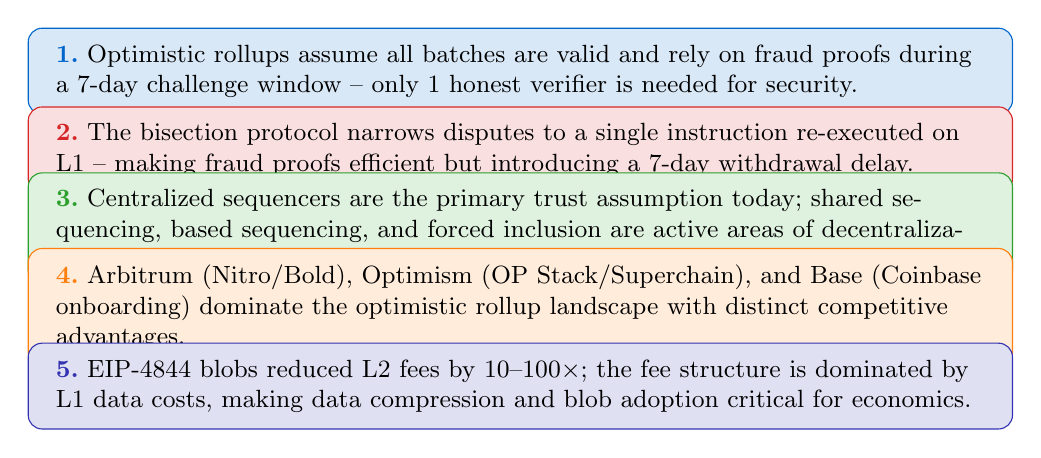
\begin{tikzpicture}[
  scale=1.0,
  every node/.style={font=\small},
  sumbox/.style={draw,rounded corners=5pt,minimum width=12.5cm,minimum height=0.85cm,
                 align=left,text width=11.8cm,inner sep=6pt},
]
  % Box 1
  \node[sumbox,fill=mlblue!15,draw=mlblue] (k1) at (6.5, 4.5) {%
    \textbf{\textcolor{mlblue}{1.}}~Optimistic rollups assume all batches are valid and rely on
    fraud proofs during a 7-day challenge window -- only 1 honest verifier is needed for security.
  };
  % Box 2
  \node[sumbox,fill=mlred!15,draw=mlred] (k2) at (6.5, 3.5) {%
    \textbf{\textcolor{mlred}{2.}}~The bisection protocol narrows disputes to a single instruction
    re-executed on L1 -- making fraud proofs efficient but introducing a 7-day withdrawal delay.
  };
  % Box 3
  \node[sumbox,fill=mlgreen!15,draw=mlgreen] (k3) at (6.5, 2.5) {%
    \textbf{\textcolor{mlgreen}{3.}}~Centralized sequencers are the primary trust assumption today;
    shared sequencing, based sequencing, and forced inclusion are active areas of decentralization research.
  };
  % Box 4
  \node[sumbox,fill=mlorange!15,draw=mlorange] (k4) at (6.5, 1.5) {%
    \textbf{\textcolor{mlorange}{4.}}~Arbitrum (Nitro/Bold), Optimism (OP Stack/Superchain), and Base
    (Coinbase onboarding) dominate the optimistic rollup landscape with distinct competitive advantages.
  };
  % Box 5
  \node[sumbox,fill=mlpurple!15,draw=mlpurple] (k5) at (6.5, 0.5) {%
    \textbf{\textcolor{mlpurple}{5.}}~EIP-4844 blobs reduced L2 fees by 10--100$\times$; the fee structure
    is dominated by L1 data costs, making data compression and blob adoption critical for economics.
  };
\end{tikzpicture}
\bottomnote{Section 2 complete -- next: Zero-Knowledge Rollups (zkSync, StarkNet, Polygon zkEVM) and validity proof mechanisms}
\end{frame}

%% ============================================================
%% SECTION 3: Zero-Knowledge Rollups
%% ============================================================
\section{Zero-Knowledge Rollups}

% Frame 26: Section 3 Divider
\begin{frame}{}
\vspace{10mm}
\begin{beamercolorbox}[sep=12pt,center,rounded=true,shadow=true]{palette quaternary}
{\Large\bfseries Section 3: Zero-Knowledge Rollups}\\[6pt]
{\normalsize Validity proofs, SNARKs vs STARKs, and the mathematical approach to scaling}
\end{beamercolorbox}
\vspace{6mm}
\begin{columns}[T]
\begin{column}{0.48\textwidth}
\begin{block}{What You Will Learn}
\begin{itemize}\setlength\itemsep{3pt}
  \item[\small$\checkmark$] \small ZK proof fundamentals: completeness, soundness, zero-knowledge
  \item[\small$\checkmark$] \small ZK-SNARKs vs ZK-STARKs: tradeoffs and trust assumptions
  \item[\small$\checkmark$] \small zkSync Era, StarkNet, and Polygon zkEVM architectures
  \item[\small$\checkmark$] \small Prover costs, hardware requirements, and proving time optimization
\end{itemize}
\end{block}
\end{column}
\begin{column}{0.48\textwidth}
\begin{block}{Frames in This Section}
\begin{itemize}\setlength\itemsep{3pt}
  \item[\small$\bullet$] \small Frame 27: ZK Proof Fundamentals
  \item[\small$\bullet$] \small Frame 28: SNARKs vs STARKs
  \item[\small$\bullet$] \small Frame 29: ZK Rollup Architecture
  \item[\small$\bullet$] \small Frame 30: ZK Proof Verification (Code)
  \item[\small$\bullet$] \small Frames 31--35: zkSync, StarkNet, Polygon, Provers, Comparison
  \item[\small$\bullet$] \small Frame 36: Section Summary
\end{itemize}
\end{block}
\end{column}
\end{columns}
\bottomnote{Section 3 of 5 -- Zero-Knowledge Rollups: prove validity with math}
\end{frame}

% Frame 27: Zero-Knowledge Proof Fundamentals
\begin{frame}{Zero-Knowledge Proof Fundamentals}
\vspace{-1mm}
\begin{columns}[T]
\column{0.48\textwidth}
\begin{block}{Three Properties of ZK Proofs}
\footnotesize
\begin{enumerate}\setlength\itemsep{4pt}
  \item \textbf{Completeness}: If the statement is true, an honest prover can always convince an honest verifier.
  \item \textbf{Soundness}: If the statement is false, no cheating prover can convince the verifier (except with negligible probability).
  \item \textbf{Zero-Knowledge}: The verifier learns \textit{nothing} beyond the truth of the statement -- no information about the witness leaks.
\end{enumerate}
\end{block}
\vspace{2mm}
\begin{alertblock}{Why It Matters for Rollups}
\footnotesize
ZK rollups use validity proofs: the prover demonstrates that all state transitions in a batch are correct \textit{without} revealing individual transaction details (though in practice, rollups post data for DA).
\end{alertblock}
\column{0.48\textwidth}
\vspace{2mm}
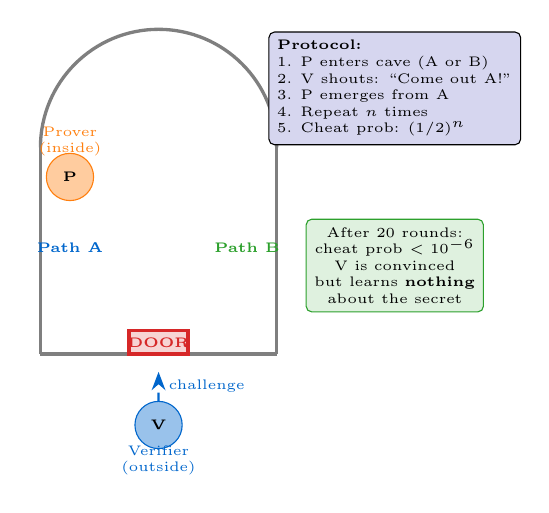
\begin{tikzpicture}[
  scale=0.75,
  every node/.style={font=\scriptsize},
  cavept/.style={draw,circle,minimum size=0.35cm,inner sep=0pt,fill=mlgray!20},
]
  % Cave outline (Ali Baba's Cave)
  \draw[very thick,mlgray] (0,0) -- (0,3.5);
  \draw[very thick,mlgray] (4,0) -- (4,3.5);
  \draw[very thick,mlgray] (0,3.5) arc (180:0:2);
  \draw[very thick,mlgray] (0,0) -- (1.5,0);
  \draw[very thick,mlgray] (2.5,0) -- (4,0);
  % Door
  \draw[very thick,mlred,fill=mlred!20] (1.5,0) rectangle (2.5,0.4);
  \node[font=\tiny\bfseries,text=mlred] at (2.0,0.2) {DOOR};
  % Path labels
  \node[font=\tiny\bfseries,text=mlblue] at (0.5,1.8) {Path A};
  \node[font=\tiny\bfseries,text=mlgreen] at (3.5,1.8) {Path B};
  % Prover (inside cave)
  \node[draw,circle,fill=mlorange!40,draw=mlorange,minimum size=0.6cm,
        inner sep=0pt,font=\tiny\bfseries] (prover) at (0.5,3.0) {P};
  \node[font=\tiny,text=mlorange,align=center] at (0.5,3.6) {Prover\\(inside)};
  % Verifier (outside)
  \node[draw,circle,fill=mlblue!40,draw=mlblue,minimum size=0.6cm,
        inner sep=0pt,font=\tiny\bfseries] (verifier) at (2.0,-1.2) {V};
  \node[font=\tiny,text=mlblue,align=center] at (2.0,-1.8) {Verifier\\(outside)};
  % Protocol steps
  \node[draw,rounded corners=2pt,fill=mllavender4,font=\tiny,align=left,
        inner sep=3pt] at (6.0,4.5) {%
    \textbf{Protocol:}\\
    1. P enters cave (A or B)\\
    2. V shouts: ``Come out A!''\\
    3. P emerges from A\\
    4. Repeat $n$ times\\
    5. Cheat prob: $(1/2)^n$%
  };
  % Arrow from verifier
  \draw[-{Stealth},thick,mlblue,dashed] (verifier.north) -- (2.0,-0.3)
    node[midway,right,font=\tiny,text=mlblue] {challenge};
  % Success annotation
  \node[draw,rounded corners=2pt,fill=mlgreen!15,draw=mlgreen,font=\tiny,
        align=center,inner sep=3pt] at (6.0,1.5) {%
    After 20 rounds:\\
    cheat prob $< 10^{-6}$\\
    V is convinced\\
    but learns \textbf{nothing}\\
    about the secret%
  };
\end{tikzpicture}
\end{columns}
\bottomnote{Ali Baba's Cave: the prover proves knowledge of the secret (door password) without ever revealing it to the verifier}
\end{frame}

% Frame 28: ZK-SNARKs vs ZK-STARKs
\begin{frame}{ZK-SNARKs vs ZK-STARKs}
\vspace{-2mm}
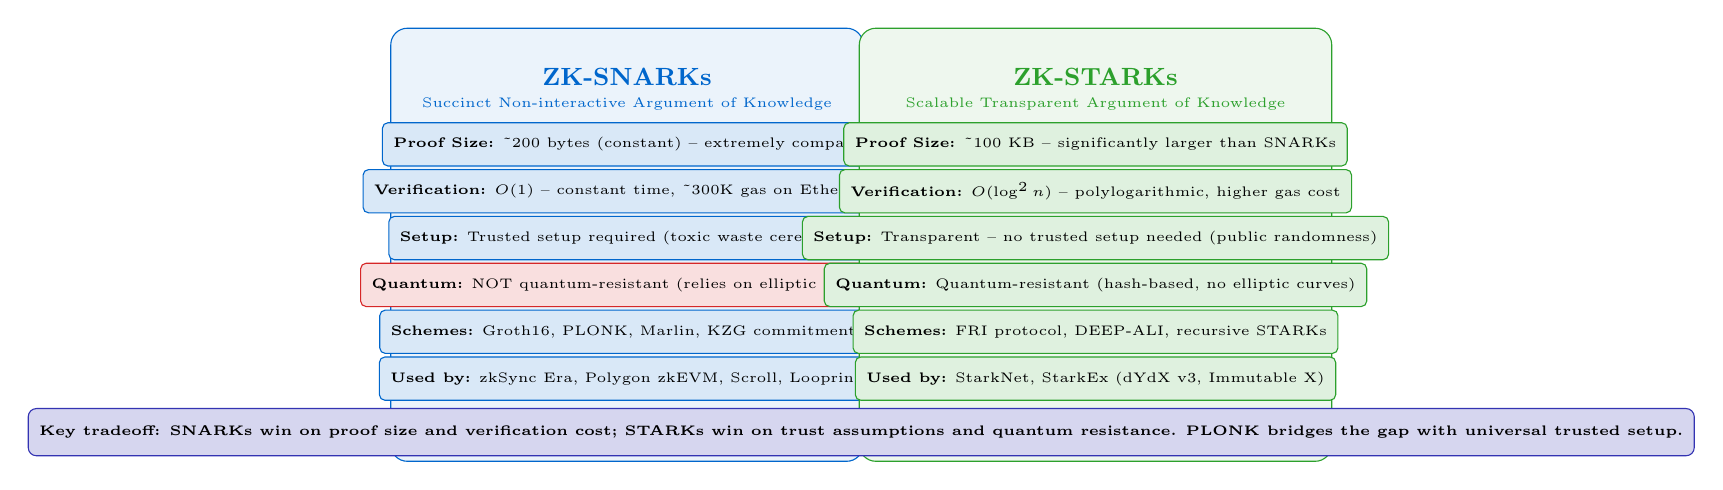
\begin{tikzpicture}[
  scale=0.85,
  every node/.style={font=\scriptsize},
  zkpanel/.style={draw,rounded corners=6pt,minimum width=6.0cm,minimum height=5.5cm,
                  inner sep=6pt,align=center},
  zkrow/.style={draw,rounded corners=2pt,minimum width=5.4cm,minimum height=0.55cm,
                align=left,inner sep=4pt,font=\tiny},
  vslabel/.style={font=\large\bfseries,text=mlgray},
]
  % SNARK panel
  \node[zkpanel,fill=mlblue!8,draw=mlblue] (snark) at (3.5,2.8) {};
  \node[font=\small\bfseries,text=mlblue] at (3.5,5.3) {ZK-SNARKs};
  \node[font=\tiny,text=mlblue] at (3.5,4.9) {Succinct Non-interactive Argument of Knowledge};

  % SNARK rows
  \node[zkrow,fill=mlblue!15,draw=mlblue] at (3.5,4.3)
    {\textbf{Proof Size:} \textasciitilde200 bytes (constant) -- extremely compact};
  \node[zkrow,fill=mlblue!15,draw=mlblue] at (3.5,3.6)
    {\textbf{Verification:} $O(1)$ -- constant time, \textasciitilde300K gas on Ethereum};
  \node[zkrow,fill=mlblue!15,draw=mlblue] at (3.5,2.9)
    {\textbf{Setup:} Trusted setup required (toxic waste ceremony)};
  \node[zkrow,fill=mlred!15,draw=mlred] at (3.5,2.2)
    {\textbf{Quantum:} NOT quantum-resistant (relies on elliptic curves)};
  \node[zkrow,fill=mlblue!15,draw=mlblue] at (3.5,1.5)
    {\textbf{Schemes:} Groth16, PLONK, Marlin, KZG commitments};
  \node[zkrow,fill=mlblue!15,draw=mlblue] at (3.5,0.8)
    {\textbf{Used by:} zkSync Era, Polygon zkEVM, Scroll, Loopring};

  % VS label
  \node[vslabel] at (7.0,2.8) {vs};

  % STARK panel
  \node[zkpanel,fill=mlgreen!8,draw=mlgreen] (stark) at (10.5,2.8) {};
  \node[font=\small\bfseries,text=mlgreen] at (10.5,5.3) {ZK-STARKs};
  \node[font=\tiny,text=mlgreen] at (10.5,4.9) {Scalable Transparent Argument of Knowledge};

  % STARK rows
  \node[zkrow,fill=mlgreen!15,draw=mlgreen] at (10.5,4.3)
    {\textbf{Proof Size:} \textasciitilde100 KB -- significantly larger than SNARKs};
  \node[zkrow,fill=mlgreen!15,draw=mlgreen] at (10.5,3.6)
    {\textbf{Verification:} $O(\log^2 n)$ -- polylogarithmic, higher gas cost};
  \node[zkrow,fill=mlgreen!15,draw=mlgreen] at (10.5,2.9)
    {\textbf{Setup:} Transparent -- no trusted setup needed (public randomness)};
  \node[zkrow,fill=mlgreen!15,draw=mlgreen] at (10.5,2.2)
    {\textbf{Quantum:} Quantum-resistant (hash-based, no elliptic curves)};
  \node[zkrow,fill=mlgreen!15,draw=mlgreen] at (10.5,1.5)
    {\textbf{Schemes:} FRI protocol, DEEP-ALI, recursive STARKs};
  \node[zkrow,fill=mlgreen!15,draw=mlgreen] at (10.5,0.8)
    {\textbf{Used by:} StarkNet, StarkEx (dYdX v3, Immutable X)};

  % Bottom comparison
  \node[draw,rounded corners=3pt,fill=mllavender4,draw=mlpurple,
        minimum width=13.0cm,minimum height=0.6cm,align=center,font=\tiny\bfseries,
        inner sep=4pt] at (7.0,0.0) {%
    Key tradeoff: SNARKs win on proof size and verification cost;
    STARKs win on trust assumptions and quantum resistance.
    PLONK bridges the gap with universal trusted setup.%
  };
\end{tikzpicture}
\bottomnote{Both are validity proofs -- they differ in cryptographic assumptions, proof size, and trust requirements}
\end{frame}

% Frame 29: ZK Rollup Architecture
\begin{frame}{ZK Rollup Architecture}
\vspace{-2mm}
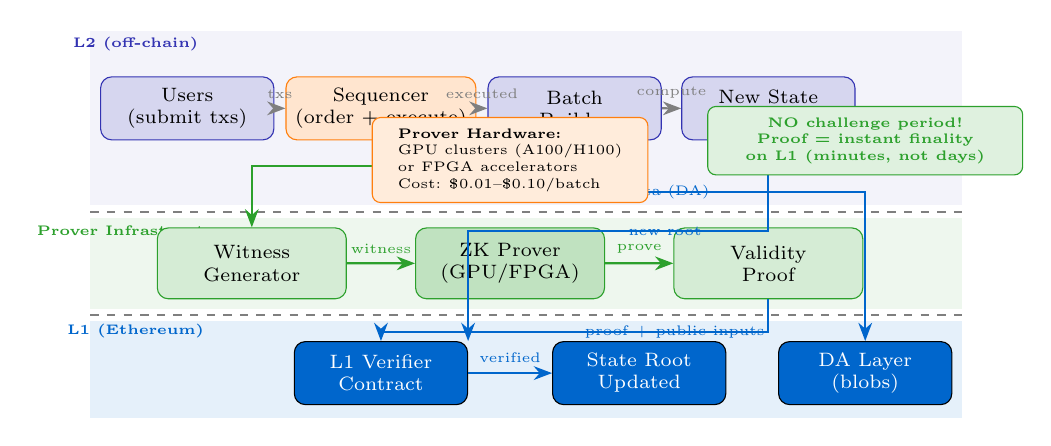
\begin{tikzpicture}[
  scale=0.82,
  every node/.style={font=\scriptsize},
  zkcomp/.style={draw,rounded corners=4pt,minimum width=2.2cm,minimum height=0.8cm,
                 align=center,fill=mllavender4,draw=mlpurple},
  l1comp/.style={draw,rounded corners=4pt,minimum width=2.2cm,minimum height=0.8cm,
                 align=center,fill=mlblue,text=white},
  proverbox/.style={draw,rounded corners=4pt,minimum width=2.4cm,minimum height=0.9cm,
                    align=center,fill=mlgreen!20,draw=mlgreen,font=\scriptsize},
  arr/.style={-{Stealth},thick,mlgray},
]
  % L2 region
  \fill[mllavender4!30] (0.0, 3.5) rectangle (13.5, 6.2);
  \node[font=\tiny\bfseries,text=mlpurple] at (0.7, 6.0) {L2 (off-chain)};

  % Prover region
  \fill[mlgreen!8] (0.0, 1.9) rectangle (13.5, 3.3);
  \node[font=\tiny\bfseries,text=mlgreen] at (0.7, 3.1) {Prover Infrastructure};

  % L1 region
  \fill[mlblue!10] (0.0, 0.2) rectangle (13.5, 1.7);
  \node[font=\tiny\bfseries,text=mlblue] at (0.7, 1.55) {L1 (Ethereum)};

  % Dashed boundaries
  \draw[dashed,thick,mlgray] (0.0, 3.4) -- (13.5, 3.4);
  \draw[dashed,thick,mlgray] (0.0, 1.8) -- (13.5, 1.8);

  % L2 components
  \node[zkcomp] (users) at (1.5, 5.0) {Users\\(submit txs)};
  \node[zkcomp,fill=mlorange!20,draw=mlorange] (seq) at (4.5, 5.0) {Sequencer\\(order + execute)};
  \node[zkcomp] (batch) at (7.5, 5.0) {Batch\\Builder};
  \node[zkcomp] (state) at (10.5, 5.0) {New State\\Root};

  % L2 flow
  \draw[arr] (users) -- (seq) node[midway,above,font=\tiny] {txs};
  \draw[arr] (seq) -- (batch) node[midway,above,font=\tiny] {executed};
  \draw[arr] (batch) -- (state) node[midway,above,font=\tiny] {compute};

  % Prover components
  \node[proverbox] (witness) at (2.5, 2.6) {Witness\\Generator};
  \node[proverbox,fill=mlgreen!30] (prover) at (6.5, 2.6) {ZK Prover\\(GPU/FPGA)};
  \node[proverbox] (proof) at (10.5, 2.6) {Validity\\Proof};

  % Batch -> Prover flow
  \draw[arr,mlgreen] (batch.south) -- ++(0,-0.4) -| (witness.north)
    node[near start,right,font=\tiny,text=mlgreen] {batch data};
  \draw[arr,mlgreen] (witness) -- (prover) node[midway,above,font=\tiny] {witness};
  \draw[arr,mlgreen] (prover) -- (proof) node[midway,above,font=\tiny] {prove};

  % L1 components
  \node[l1comp] (verifier) at (4.5, 0.9) {L1 Verifier\\Contract};
  \node[l1comp] (stateroot) at (8.5, 0.9) {State Root\\Updated};
  \node[l1comp] (blobda) at (12.0, 0.9) {DA Layer\\(blobs)};

  % Proof -> L1
  \draw[arr,mlblue,thick] (proof.south) -- ++(0,-0.5) -| (verifier.north)
    node[near start,right,font=\tiny,text=mlblue] {proof + public inputs};
  \draw[arr,mlblue,thick] (state.south) -- ++(0,-1.4) -| (verifier.north east)
    node[near start,right,font=\tiny,text=mlblue] {new root};
  \draw[arr,mlblue] (verifier) -- (stateroot)
    node[midway,above,font=\tiny] {verified};
  \draw[arr,mlblue] (batch.south) -- ++(0,-0.8) -| (blobda.north)
    node[near start,left,font=\tiny,text=mlblue] {tx data (DA)};

  % Key difference callout
  \node[draw,fill=mlgreen!15,draw=mlgreen,rounded corners=3pt,
        minimum width=4.0cm,align=center,font=\tiny\bfseries,inner sep=4pt,
        text=mlgreen] at (12.0, 4.5) {%
    NO challenge period!\\
    Proof = instant finality\\
    on L1 (minutes, not days)%
  };

  % Prover hardware callout
  \node[draw,fill=mlorange!15,draw=mlorange,rounded corners=3pt,
        minimum width=3.5cm,align=left,font=\tiny,inner sep=4pt]
    at (6.5, 4.2) {%
    \textbf{Prover Hardware:}\\
    GPU clusters (A100/H100)\\
    or FPGA accelerators\\
    Cost: \$0.01--\$0.10/batch%
  };
\end{tikzpicture}
\bottomnote{ZK rollups replace the 7-day challenge window with a mathematical proof -- instant L1 finality once the proof is verified}
\end{frame}

% Frame 30: ZK Proof Verification [FRAGILE] -- CODE FRAME
\begin{frame}[fragile]{ZK Proof Verification}
\begin{columns}[T]
\column{0.50\textwidth}
\vspace{1mm}
\begin{lstlisting}[language=Solidity,caption={Simplified ZK Verifier}]
// Simplified ZK Verifier
contract ZKRollupVerifier {
    bytes32 public stateRoot;
    uint256 public batchNumber;

    function verifyAndUpdate(
        bytes32 newStateRoot,
        uint256[2] memory proofA,
        uint256[2][2] memory proofB,
        uint256[2] memory proofC,
        uint256[] memory publicInputs
    ) external {
        require(
            verifyProof(
                proofA, proofB, proofC,
                publicInputs
            ),
            "Invalid ZK proof"
        );
        stateRoot = newStateRoot;
        batchNumber++;
        emit StateUpdated(
            batchNumber, newStateRoot);
    }
}
\end{lstlisting}
\column{0.50\textwidth}
\vspace{2mm}
\begin{block}{Pairing-Based Verification}
\footnotesize
\begin{itemize}
  \item \textbf{Groth16}: 3 elliptic curve pairings, \textasciitilde200K gas, circuit-specific trusted setup
  \item \textbf{PLONK}: Universal setup (reusable), slightly higher gas (\textasciitilde300K), more flexible
  \item \textbf{Verification}: L1 contract checks $e(A, B) = e(\alpha, \beta) \cdot e(L, \gamma) \cdot e(C, \delta)$
  \item \textbf{Public inputs}: Previous state root, new state root, batch hash
\end{itemize}
\end{block}
\vspace{2mm}
\begin{block}{Gas Cost Comparison}
\footnotesize
\begin{itemize}
  \item ZK proof verification: \textasciitilde300K gas (fixed cost per batch)
  \item Optimistic batch posting: \textasciitilde40K gas (but 7-day delay)
  \item ZK amortized per tx: \$0.001--\$0.01 (spread across 1000s of txs)
  \item Cost dominated by \textbf{prover computation}, not verification
\end{itemize}
\end{block}
\vspace{2mm}
\begin{alertblock}{Key Insight}
\footnotesize
Verification is $O(1)$ regardless of batch size -- a batch of 10 txs costs the same to verify as 10{,}000 txs. The prover bears the scaling cost.
\end{alertblock}
\end{columns}
\bottomnote{ZK verification on L1 costs fixed gas per batch -- the more transactions per batch, the cheaper per-transaction cost}
\end{frame}

% Frame 31: zkSync Era
\begin{frame}{zkSync Era}
\vspace{-1mm}
\begin{columns}[T]
\column{0.48\textwidth}
\begin{block}{Architecture Overview}
\footnotesize
\begin{itemize}\setlength\itemsep{3pt}
  \item \textbf{zkEVM type}: Bytecode-level compatible (compiles Solidity via zksolc to custom bytecodes, then proves)
  \item \textbf{Proof system}: Boojum (PLONK-based with FRI), replaced previous Bellman prover
  \item \textbf{Native Account Abstraction}: Every account is a smart contract -- no EOAs, built-in paymasters
  \item \textbf{ZK Stack}: Open-source modular framework for building custom ZK chains (Hyperchains)
  \item \textbf{Data Availability}: Posts to Ethereum L1 (rollup mode) or DA committee (validium mode)
  \item \textbf{Token}: ZK (governance, launched June 2024)
\end{itemize}
\end{block}
\vspace{1mm}
\begin{alertblock}{Key Innovation}
\footnotesize
Native AA means gasless transactions, session keys, and social recovery are protocol-level features, not afterthoughts.
\end{alertblock}
\column{0.48\textwidth}
\vspace{2mm}
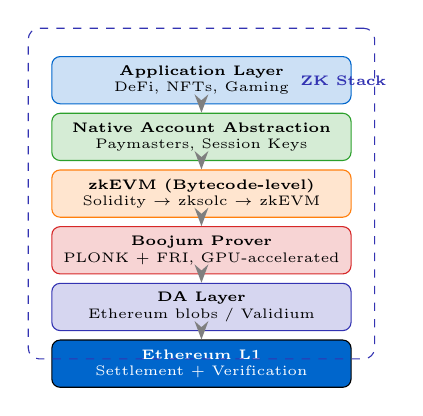
\begin{tikzpicture}[
  scale=0.72,
  every node/.style={font=\tiny},
  zkblock/.style={draw,rounded corners=3pt,minimum width=3.8cm,minimum height=0.6cm,
                  align=center,inner sep=3pt},
  arr/.style={-{Stealth},thick,mlgray},
]
  % Stack layers
  \node[zkblock,fill=mlblue!20,draw=mlblue] (app) at (2.2,5.5)
    {\textbf{Application Layer}\\DeFi, NFTs, Gaming};
  \node[zkblock,fill=mlgreen!20,draw=mlgreen] (aa) at (2.2,4.5)
    {\textbf{Native Account Abstraction}\\Paymasters, Session Keys};
  \node[zkblock,fill=mlorange!20,draw=mlorange] (vm) at (2.2,3.5)
    {\textbf{zkEVM (Bytecode-level)}\\Solidity $\rightarrow$ zksolc $\rightarrow$ zkEVM};
  \node[zkblock,fill=mlred!20,draw=mlred] (prover) at (2.2,2.5)
    {\textbf{Boojum Prover}\\PLONK + FRI, GPU-accelerated};
  \node[zkblock,fill=mlpurple!20,draw=mlpurple] (da) at (2.2,1.5)
    {\textbf{DA Layer}\\Ethereum blobs / Validium};
  \node[zkblock,fill=mlblue,text=white] (l1) at (2.2,0.5)
    {\textbf{Ethereum L1}\\Settlement + Verification};

  % Arrows
  \draw[arr] (app) -- (aa);
  \draw[arr] (aa) -- (vm);
  \draw[arr] (vm) -- (prover);
  \draw[arr] (prover) -- (da);
  \draw[arr] (da) -- (l1);

  % ZK Stack label
  \node[draw,dashed,rounded corners=4pt,draw=mlpurple,
        minimum width=4.4cm,minimum height=4.2cm,inner sep=0pt]
    at (2.2,3.5) {};
  \node[font=\tiny\bfseries,text=mlpurple] at (4.7,5.5) {ZK Stack};
\end{tikzpicture}
\end{columns}
\bottomnote{zkSync Era pioneered native account abstraction and the ZK Stack framework for building sovereign ZK rollups}
\end{frame}

% Frame 32: StarkNet and Cairo
\begin{frame}{StarkNet \& Cairo}
\vspace{-1mm}
\begin{columns}[T]
\column{0.48\textwidth}
\begin{block}{Architecture Overview}
\footnotesize
\begin{itemize}\setlength\itemsep{3pt}
  \item \textbf{Proof system}: ZK-STARKs -- no trusted setup, quantum-resistant, transparent
  \item \textbf{Language}: Cairo -- purpose-built for provable computation (not EVM-compatible by default)
  \item \textbf{Recursive proofs}: SHARP (Shared Prover) aggregates proofs from multiple apps into one L1 proof
  \item \textbf{Execution model}: Cairo VM (not EVM) -- different programming paradigm optimized for proof generation
  \item \textbf{Appchains}: StarkNet Stack allows building application-specific chains with shared proving
  \item \textbf{Token}: STRK (governance + fees, launched Feb 2024)
\end{itemize}
\end{block}
\vspace{1mm}
\begin{alertblock}{Key Innovation}
\footnotesize
SHARP lets multiple applications (StarkNet, dYdX v3, Immutable X, Sorare) share one prover and split verification costs on L1.
\end{alertblock}
\column{0.48\textwidth}
\vspace{2mm}
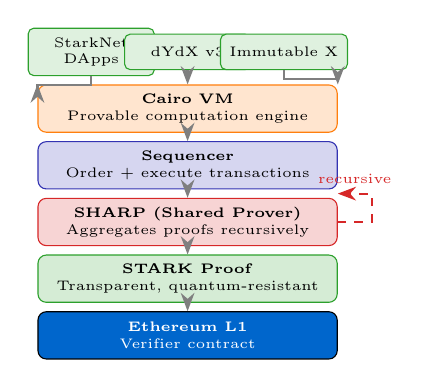
\begin{tikzpicture}[
  scale=0.72,
  every node/.style={font=\tiny},
  snblock/.style={draw,rounded corners=3pt,minimum width=3.8cm,minimum height=0.6cm,
                  align=center,inner sep=3pt},
  appnode/.style={draw,rounded corners=2pt,minimum width=1.6cm,minimum height=0.45cm,
                  align=center,fill=mlgreen!15,draw=mlgreen,font=\tiny},
  arr/.style={-{Stealth},thick,mlgray},
]
  % Application layer
  \node[appnode] (app1) at (0.5,5.5) {StarkNet\\DApps};
  \node[appnode] (app2) at (2.2,5.5) {dYdX v3};
  \node[appnode] (app3) at (3.9,5.5) {Immutable X};

  % Cairo VM
  \node[snblock,fill=mlorange!20,draw=mlorange] (cairo) at (2.2,4.5)
    {\textbf{Cairo VM}\\Provable computation engine};

  % Sequencer
  \node[snblock,fill=mlpurple!20,draw=mlpurple] (seq) at (2.2,3.5)
    {\textbf{Sequencer}\\Order + execute transactions};

  % SHARP
  \node[snblock,fill=mlred!20,draw=mlred] (sharp) at (2.2,2.5)
    {\textbf{SHARP (Shared Prover)}\\Aggregates proofs recursively};

  % STARK proof
  \node[snblock,fill=mlgreen!20,draw=mlgreen] (proof) at (2.2,1.5)
    {\textbf{STARK Proof}\\Transparent, quantum-resistant};

  % L1
  \node[snblock,fill=mlblue,text=white] (l1) at (2.2,0.5)
    {\textbf{Ethereum L1}\\Verifier contract};

  % Arrows
  \draw[arr] (app1.south) -- ++(0,-0.15) -| (cairo.north west);
  \draw[arr] (app2.south) -- (cairo.north);
  \draw[arr] (app3.south) -- ++(0,-0.15) -| (cairo.north east);
  \draw[arr] (cairo) -- (seq);
  \draw[arr] (seq) -- (sharp);
  \draw[arr] (sharp) -- (proof);
  \draw[arr] (proof) -- (l1);

  % Recursive label
  \draw[-{Stealth},dashed,mlred,thick] (sharp.east) -- ++(0.6,0) -- ++(0,0.5)
    -- ++(-0.6,0) node[midway,above,font=\tiny,text=mlred] {recursive};
\end{tikzpicture}
\end{columns}
\bottomnote{StarkNet uses STARKs for quantum-resistant proofs and Cairo for provable computation -- SHARP amortizes L1 costs across apps}
\end{frame}

% Frame 33: Polygon zkEVM
\begin{frame}{Polygon zkEVM}
\vspace{-1mm}
\begin{columns}[T]
\column{0.48\textwidth}
\begin{block}{Architecture Overview}
\footnotesize
\begin{itemize}\setlength\itemsep{3pt}
  \item \textbf{zkEVM type}: Type 2 -- full EVM equivalence at the opcode level (existing Solidity contracts deploy without changes)
  \item \textbf{Proving time}: \textasciitilde10 minutes per batch (improving with recursive proofs and hardware acceleration)
  \item \textbf{Proof system}: Custom SNARK (FFLONK variant with recursive composition)
  \item \textbf{AggLayer}: Unified bridge and proof aggregation layer connecting all Polygon chains
  \item \textbf{CDK (Chain Development Kit)}: Build sovereign ZK L2s with shared liquidity via AggLayer
  \item \textbf{Polygon 2.0}: Vision for network of ZK-connected chains with unified liquidity
\end{itemize}
\end{block}
\vspace{1mm}
\begin{alertblock}{Key Innovation}
\footnotesize
Type 2 zkEVM means zero migration cost -- any Ethereum dApp works on Polygon zkEVM with no code changes. AggLayer unifies liquidity.
\end{alertblock}
\column{0.48\textwidth}
\vspace{2mm}
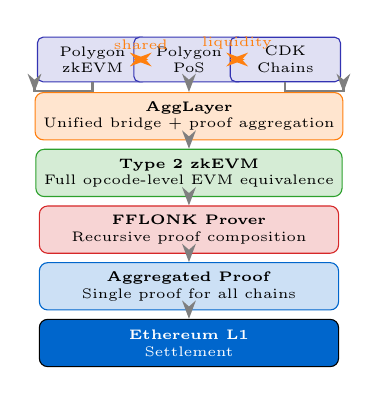
\begin{tikzpicture}[
  scale=0.72,
  every node/.style={font=\tiny},
  pgblock/.style={draw,rounded corners=3pt,minimum width=3.8cm,minimum height=0.6cm,
                  align=center,inner sep=3pt},
  chainnode/.style={draw,rounded corners=2pt,minimum width=1.4cm,minimum height=0.45cm,
                    align=center,fill=mlpurple!15,draw=mlpurple,font=\tiny},
  arr/.style={-{Stealth},thick,mlgray},
]
  % Polygon 2.0 chains
  \node[chainnode] (c1) at (0.5,5.5) {Polygon\\zkEVM};
  \node[chainnode] (c2) at (2.2,5.5) {Polygon\\PoS};
  \node[chainnode] (c3) at (3.9,5.5) {CDK\\Chains};

  % AggLayer
  \node[pgblock,fill=mlorange!20,draw=mlorange] (agg) at (2.2,4.5)
    {\textbf{AggLayer}\\Unified bridge + proof aggregation};

  % zkEVM engine
  \node[pgblock,fill=mlgreen!20,draw=mlgreen] (zkevm) at (2.2,3.5)
    {\textbf{Type 2 zkEVM}\\Full opcode-level EVM equivalence};

  % Prover
  \node[pgblock,fill=mlred!20,draw=mlred] (prover) at (2.2,2.5)
    {\textbf{FFLONK Prover}\\Recursive proof composition};

  % Aggregated proof
  \node[pgblock,fill=mlblue!20,draw=mlblue] (aggproof) at (2.2,1.5)
    {\textbf{Aggregated Proof}\\Single proof for all chains};

  % L1
  \node[pgblock,fill=mlblue,text=white] (l1) at (2.2,0.5)
    {\textbf{Ethereum L1}\\Settlement};

  % Arrows
  \draw[arr] (c1.south) -- ++(0,-0.15) -| (agg.north west);
  \draw[arr] (c2.south) -- (agg.north);
  \draw[arr] (c3.south) -- ++(0,-0.15) -| (agg.north east);
  \draw[arr] (agg) -- (zkevm);
  \draw[arr] (zkevm) -- (prover);
  \draw[arr] (prover) -- (aggproof);
  \draw[arr] (aggproof) -- (l1);

  % Shared liquidity annotation
  \draw[{Stealth}-{Stealth},dashed,mlorange,thick]
    (c1.east) -- (c2.west) node[midway,above,font=\tiny,text=mlorange] {shared};
  \draw[{Stealth}-{Stealth},dashed,mlorange,thick]
    (c2.east) -- (c3.west) node[midway,above,font=\tiny,text=mlorange] {liquidity};
\end{tikzpicture}
\end{columns}
\bottomnote{Polygon zkEVM offers full Solidity compatibility with zero migration cost -- AggLayer connects all Polygon chains with shared liquidity}
\end{frame}

% Frame 34: Prover Economics
\begin{frame}{Prover Economics}
\vspace{-2mm}
\begin{columns}[T]
\column{0.48\textwidth}
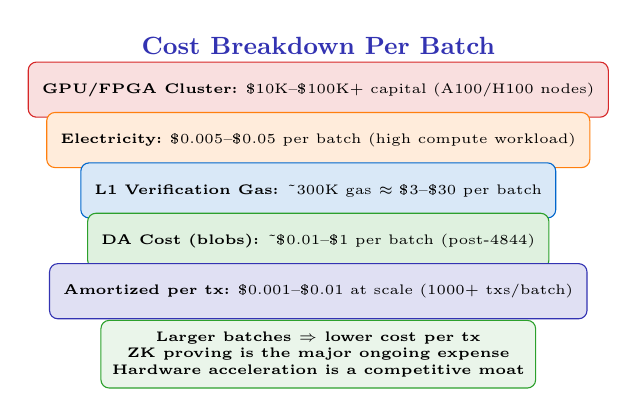
\begin{tikzpicture}[
  scale=0.80,
  every node/.style={font=\scriptsize},
  costbox/.style={draw,rounded corners=3pt,minimum width=5.2cm,minimum height=0.7cm,
                  align=left,inner sep=5pt,font=\tiny},
]
  % Title
  \node[font=\small\bfseries,text=mlpurple] at (2.8,5.5) {Cost Breakdown Per Batch};

  % Cost rows
  \node[costbox,fill=mlred!15,draw=mlred] at (2.8,4.8)
    {\textbf{GPU/FPGA Cluster:} \$10K--\$100K+ capital (A100/H100 nodes)};
  \node[costbox,fill=mlorange!15,draw=mlorange] at (2.8,4.0)
    {\textbf{Electricity:} \$0.005--\$0.05 per batch (high compute workload)};
  \node[costbox,fill=mlblue!15,draw=mlblue] at (2.8,3.2)
    {\textbf{L1 Verification Gas:} \textasciitilde300K gas $\approx$ \$3--\$30 per batch};
  \node[costbox,fill=mlgreen!15,draw=mlgreen] at (2.8,2.4)
    {\textbf{DA Cost (blobs):} \textasciitilde\$0.01--\$1 per batch (post-4844)};
  \node[costbox,fill=mlpurple!15,draw=mlpurple] at (2.8,1.6)
    {\textbf{Amortized per tx:} \$0.001--\$0.01 at scale (1000+ txs/batch)};

  % Key insight
  \node[draw,fill=mlgreen!10,draw=mlgreen,rounded corners=3pt,
        minimum width=5.2cm,align=center,font=\tiny\bfseries,inner sep=4pt]
    at (2.8,0.6) {%
    Larger batches $\Rightarrow$ lower cost per tx\\
    ZK proving is the major ongoing expense\\
    Hardware acceleration is a competitive moat%
  };
\end{tikzpicture}
\column{0.48\textwidth}
\vspace{2mm}
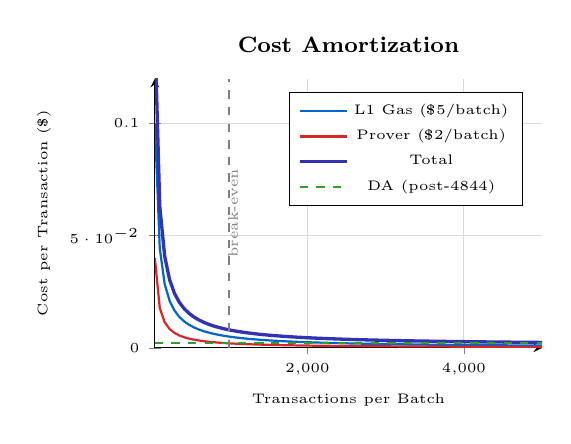
\begin{tikzpicture}
\begin{axis}[
  width=6.5cm,
  height=5.0cm,
  xlabel={Transactions per Batch},
  ylabel={Cost per Transaction (\$)},
  title={\footnotesize Cost Amortization},
  xmin=50, xmax=5000,
  ymin=0, ymax=0.12,
  grid=major,
  grid style={mlgray!30},
  axis lines=left,
  xlabel style={font=\tiny},
  ylabel style={font=\tiny},
  title style={font=\scriptsize\bfseries},
  tick label style={font=\tiny},
  legend style={font=\tiny,at={(0.95,0.95)},anchor=north east},
]
  % L1 gas cost curve (hyperbolic: fixed cost / batch size)
  \addplot[mlblue,thick,domain=50:5000,samples=80] {5/x};
  \addlegendentry{L1 Gas (\$5/batch)}

  % Prover cost curve
  \addplot[mlred,thick,domain=50:5000,samples=80] {2/x};
  \addlegendentry{Prover (\$2/batch)}

  % Total cost curve
  \addplot[mlpurple,very thick,domain=50:5000,samples=80] {7/x + 0.001};
  \addlegendentry{Total}

  % DA cost (flat per tx after 4844)
  \addplot[mlgreen,thick,dashed,domain=50:5000,samples=80] {0.002};
  \addlegendentry{DA (post-4844)}

  % Break-even annotation
  \draw[mlgray,dashed,thick] (axis cs:1000,0) -- (axis cs:1000,0.12);
  \node[font=\tiny,text=mlgray,rotate=90] at (axis cs:1050,0.06) {break-even};
\end{axis}
\end{tikzpicture}
\end{columns}
\bottomnote{ZK prover costs are amortized across all transactions in a batch -- economies of scale make larger batches dramatically cheaper per tx}
\end{frame}

% Frame 35: ZK Rollup Comparison Table
\begin{frame}{ZK Rollup Comparison}
\vspace{-1mm}
\begin{adjustbox}{max width=\textwidth}
\begin{tabular}{l >{\small}c >{\small}c >{\small}c}
\toprule
\textbf{Feature} & \textbf{zkSync Era} & \textbf{StarkNet} & \textbf{Polygon zkEVM} \\
\midrule
Proof System & PLONK + FRI (Boojum) & STARKs (SHARP) & FFLONK (recursive) \\
EVM Compatibility & Bytecode-level (Type 4) & None (Cairo VM) & Opcode-level (Type 2) \\
Smart Contract Language & Solidity (via zksolc) & Cairo & Solidity (native) \\
Trusted Setup & Yes (universal/PLONK) & No (transparent) & Yes (universal/PLONK) \\
Quantum Resistant & No & Yes & No \\
Finality (to L1) & \textasciitilde1 hour & \textasciitilde2--4 hours & \textasciitilde30 min \\
TVL (2024 peak) & \textasciitilde\$1B & \textasciitilde\$200M & \textasciitilde\$100M \\
Avg Fee (post-4844) & \$0.01--\$0.10 & \$0.01--\$0.05 & \$0.01--\$0.05 \\
Key Innovation & Native AA, ZK Stack & SHARP, Cairo lang & Type 2 zkEVM, AggLayer \\
Appchain Framework & ZK Stack (Hyperchains) & StarkNet Stack & CDK (Chain Dev Kit) \\
Prover Hardware & GPU (Boojum) & CPU + GPU (Stone) & GPU (FFLONK) \\
\bottomrule
\end{tabular}
\end{adjustbox}
\vspace{4mm}
\begin{columns}[T]
\column{0.33\textwidth}
\begin{block}{\footnotesize zkSync Strengths}
\scriptsize
\begin{itemize}
  \item Native Account Abstraction
  \item ZK Stack for sovereign chains
  \item Boojum: efficient GPU proving
\end{itemize}
\end{block}
\column{0.33\textwidth}
\begin{block}{\footnotesize StarkNet Strengths}
\scriptsize
\begin{itemize}
  \item No trusted setup (transparent)
  \item Quantum-resistant proofs
  \item SHARP: shared proving costs
\end{itemize}
\end{block}
\column{0.33\textwidth}
\begin{block}{\footnotesize Polygon zkEVM Strengths}
\scriptsize
\begin{itemize}
  \item Full Solidity compatibility
  \item AggLayer: unified liquidity
  \item CDK for custom L2 chains
\end{itemize}
\end{block}
\end{columns}
\bottomnote{Each ZK rollup makes different tradeoffs -- zkSync (AA), StarkNet (STARKs), Polygon (EVM compat) -- all settling on Ethereum}
\end{frame}

% Frame 36: Section 3 Summary
\begin{frame}{Section 3 Summary}
\vspace{2mm}
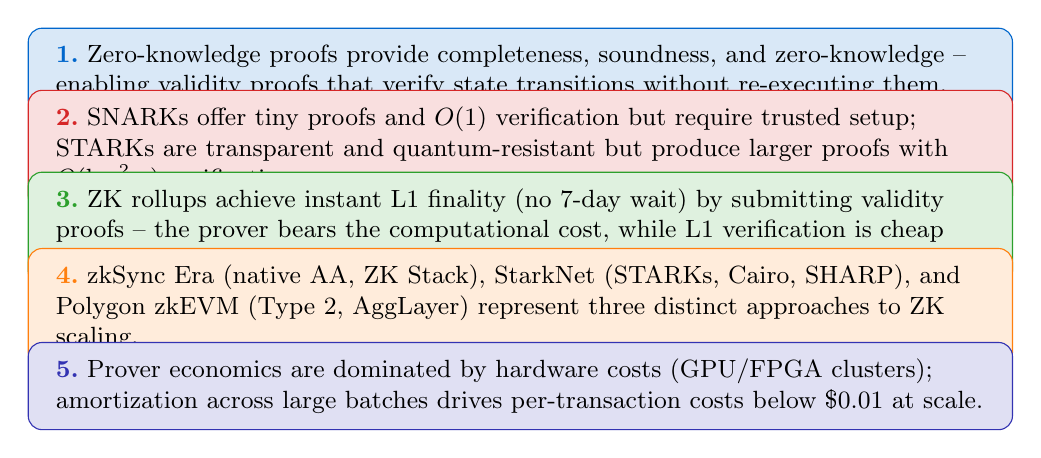
\begin{tikzpicture}[
  scale=1.0,
  every node/.style={font=\small},
  sumbox/.style={draw,rounded corners=5pt,minimum width=12.5cm,minimum height=0.85cm,
                 align=left,text width=11.8cm,inner sep=6pt},
]
  % Box 1
  \node[sumbox,fill=mlblue!15,draw=mlblue] (k1) at (6.5, 4.5) {%
    \textbf{\textcolor{mlblue}{1.}}~Zero-knowledge proofs provide completeness, soundness, and zero-knowledge --
    enabling validity proofs that verify state transitions without re-executing them.
  };
  % Box 2
  \node[sumbox,fill=mlred!15,draw=mlred] (k2) at (6.5, 3.5) {%
    \textbf{\textcolor{mlred}{2.}}~SNARKs offer tiny proofs and $O(1)$ verification but require trusted setup;
    STARKs are transparent and quantum-resistant but produce larger proofs with $O(\log^2 n)$ verification.
  };
  % Box 3
  \node[sumbox,fill=mlgreen!15,draw=mlgreen] (k3) at (6.5, 2.5) {%
    \textbf{\textcolor{mlgreen}{3.}}~ZK rollups achieve instant L1 finality (no 7-day wait) by submitting validity proofs --
    the prover bears the computational cost, while L1 verification is cheap and constant-time.
  };
  % Box 4
  \node[sumbox,fill=mlorange!15,draw=mlorange] (k4) at (6.5, 1.5) {%
    \textbf{\textcolor{mlorange}{4.}}~zkSync Era (native AA, ZK Stack), StarkNet (STARKs, Cairo, SHARP),
    and Polygon zkEVM (Type 2, AggLayer) represent three distinct approaches to ZK scaling.
  };
  % Box 5
  \node[sumbox,fill=mlpurple!15,draw=mlpurple] (k5) at (6.5, 0.5) {%
    \textbf{\textcolor{mlpurple}{5.}}~Prover economics are dominated by hardware costs (GPU/FPGA clusters);
    amortization across large batches drives per-transaction costs below \$0.01 at scale.
  };
\end{tikzpicture}
\bottomnote{Section 3 complete -- next: Sidechains \& Alternative Scaling approaches}
\end{frame}

%% ============================================================
%% SECTION 4: Sidechains & Alternative Scaling
%% ============================================================
\section{Sidechains \& Alternative Scaling}

% Frame 37: Section 4 Divider
\begin{frame}{}
\vspace{10mm}
\begin{beamercolorbox}[sep=12pt,center,rounded=true,shadow=true]{palette quaternary}
{\Large\bfseries Section 4: Sidechains \& Alternative Scaling}\\[6pt]
{\normalsize Beyond rollups: sidechains, modular blockchains, and data availability innovations}
\end{beamercolorbox}
\vspace{6mm}
\begin{columns}[T]
\begin{column}{0.48\textwidth}
\begin{block}{What You Will Learn}
\begin{itemize}\setlength\itemsep{3pt}
  \item[\small$\checkmark$] \small Sidechains vs rollups: trust models and security tradeoffs
  \item[\small$\checkmark$] \small Polygon PoS and Avalanche subnet architectures
  \item[\small$\checkmark$] \small The modular blockchain thesis and separation of concerns
  \item[\small$\checkmark$] \small EIP-4844 blobs, Celestia, and data availability innovations
\end{itemize}
\end{block}
\end{column}
\begin{column}{0.48\textwidth}
\begin{block}{Frames in This Section}
\begin{itemize}\setlength\itemsep{3pt}
  \item[\small$\bullet$] \small Frame 38: Sidechains vs Rollups
  \item[\small$\bullet$] \small Frame 39: Polygon PoS
  \item[\small$\bullet$] \small Frame 40: Avalanche Subnets
  \item[\small$\bullet$] \small Frame 41: Modular Blockchain Thesis
  \item[\small$\bullet$] \small Frame 42: Bridge Contract (Code)
  \item[\small$\bullet$] \small Frames 43--46: EIP-4844, Celestia, Danksharding, Validiums
  \item[\small$\bullet$] \small Frame 47: Section Summary
\end{itemize}
\end{block}
\end{column}
\end{columns}
\bottomnote{Section 4 of 5 -- Sidechains \& Alternative Scaling: beyond rollups}
\end{frame}

% Frame 38: Sidechains vs Rollups
\begin{frame}{Sidechains vs Rollups}
\vspace{-1mm}
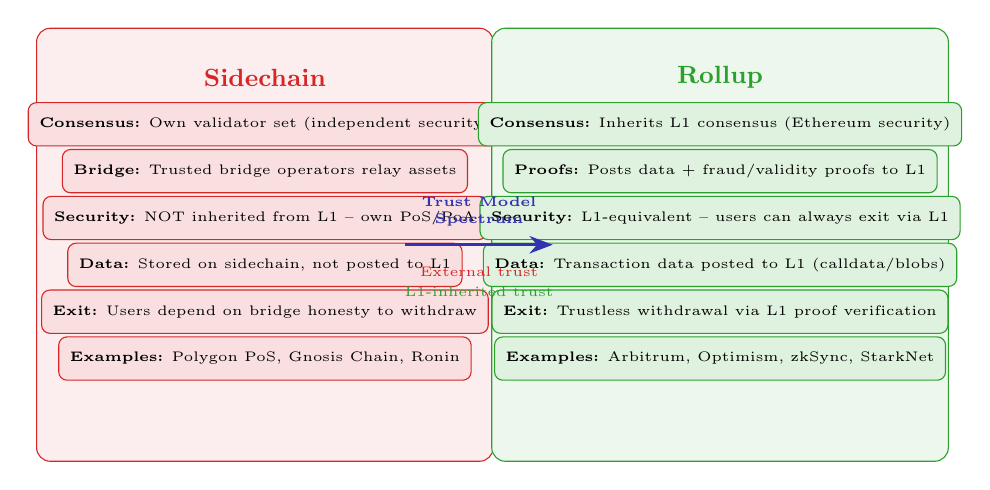
\begin{tikzpicture}[
  scale=0.85,
  every node/.style={font=\scriptsize},
  panelbox/.style={draw,rounded corners=5pt,minimum width=5.8cm,minimum height=5.5cm,
                   align=center,inner sep=6pt},
  propbox/.style={draw,rounded corners=3pt,minimum width=5.0cm,minimum height=0.55cm,
                  align=left,inner sep=4pt,font=\tiny},
]
  % Left panel: Sidechain
  \node[panelbox,fill=mlred!8,draw=mlred] (sc) at (3.2,3.0) {};
  \node[font=\small\bfseries,text=mlred] at (3.2,5.5) {Sidechain};

  \node[propbox,fill=mlred!15,draw=mlred] at (3.2,4.8)
    {\textbf{Consensus:} Own validator set (independent security)};
  \node[propbox,fill=mlred!15,draw=mlred] at (3.2,4.1)
    {\textbf{Bridge:} Trusted bridge operators relay assets};
  \node[propbox,fill=mlred!15,draw=mlred] at (3.2,3.4)
    {\textbf{Security:} NOT inherited from L1 -- own PoS/PoA};
  \node[propbox,fill=mlred!15,draw=mlred] at (3.2,2.7)
    {\textbf{Data:} Stored on sidechain, not posted to L1};
  \node[propbox,fill=mlred!15,draw=mlred] at (3.2,2.0)
    {\textbf{Exit:} Users depend on bridge honesty to withdraw};
  \node[propbox,fill=mlred!15,draw=mlred] at (3.2,1.3)
    {\textbf{Examples:} Polygon PoS, Gnosis Chain, Ronin};

  % Right panel: Rollup
  \node[panelbox,fill=mlgreen!8,draw=mlgreen] (ru) at (10.0,3.0) {};
  \node[font=\small\bfseries,text=mlgreen] at (10.0,5.5) {Rollup};

  \node[propbox,fill=mlgreen!15,draw=mlgreen] at (10.0,4.8)
    {\textbf{Consensus:} Inherits L1 consensus (Ethereum security)};
  \node[propbox,fill=mlgreen!15,draw=mlgreen] at (10.0,4.1)
    {\textbf{Proofs:} Posts data + fraud/validity proofs to L1};
  \node[propbox,fill=mlgreen!15,draw=mlgreen] at (10.0,3.4)
    {\textbf{Security:} L1-equivalent -- users can always exit via L1};
  \node[propbox,fill=mlgreen!15,draw=mlgreen] at (10.0,2.7)
    {\textbf{Data:} Transaction data posted to L1 (calldata/blobs)};
  \node[propbox,fill=mlgreen!15,draw=mlgreen] at (10.0,2.0)
    {\textbf{Exit:} Trustless withdrawal via L1 proof verification};
  \node[propbox,fill=mlgreen!15,draw=mlgreen] at (10.0,1.3)
    {\textbf{Examples:} Arbitrum, Optimism, zkSync, StarkNet};

  % Center trust model arrow
  \draw[-{Stealth},very thick,mlpurple] (5.3,3.0) -- (7.5,3.0);
  \node[font=\tiny\bfseries,text=mlpurple,align=center] at (6.4,3.5) {Trust Model\\Spectrum};
  \node[font=\tiny,text=mlred] at (6.4,2.6) {External trust};
  \node[font=\tiny,text=mlgreen] at (6.4,2.3) {L1-inherited trust};
\end{tikzpicture}
\bottomnote{Sidechains have independent security; rollups inherit L1 security -- the key distinction is the trust model for withdrawals}
\end{frame}

% Frame 39: Polygon PoS
\begin{frame}{Polygon PoS}
\vspace{-1mm}
\begin{columns}[T]
\column{0.48\textwidth}
\begin{block}{Architecture Overview}
\footnotesize
\begin{itemize}\setlength\itemsep{3pt}
  \item \textbf{Validator Set}: \textasciitilde100 validators running Proof of Stake
  \item \textbf{Heimdall Layer}: Tendermint-based consensus for checkpointing
  \item \textbf{Bor Layer}: Block production (modified Geth, EVM-compatible)
  \item \textbf{Checkpoints}: Periodic state commitments to Ethereum L1
  \item \textbf{Bridge}: PoS bridge for asset transfers (trusted validator set)
\end{itemize}
\end{block}
\vspace{2mm}
\begin{block}{Transition to zkEVM}
\footnotesize
\begin{itemize}
  \item Polygon PoS transitioning to a \textbf{validium} secured by ZK proofs
  \item \textbf{AggLayer}: Unified bridge aggregating ZK proofs from multiple chains
  \item Goal: Sidechain convenience with rollup-level security
  \item POL token replacing MATIC for expanded utility
\end{itemize}
\end{block}
\column{0.48\textwidth}
\vspace{1mm}
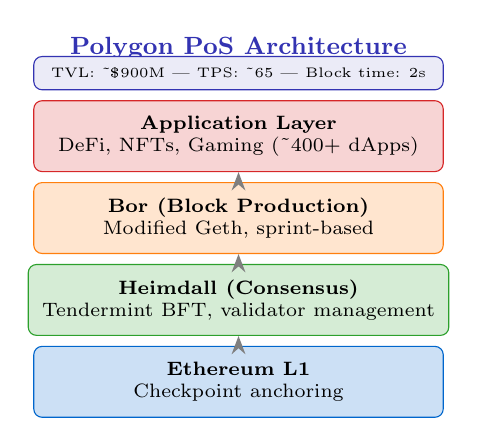
\begin{tikzpicture}[
  scale=0.80,
  every node/.style={font=\scriptsize},
  stackbox/.style={draw,rounded corners=3pt,minimum width=5.2cm,minimum height=0.9cm,
                   align=center,inner sep=5pt},
]
  % Title
  \node[font=\small\bfseries,text=mlpurple] at (2.8,5.8) {Polygon PoS Architecture};

  % Stack layers
  \node[stackbox,fill=mlblue!20,draw=mlblue] (l1) at (2.8,0.5)
    {\textbf{Ethereum L1}\\Checkpoint anchoring};
  \node[stackbox,fill=mlgreen!20,draw=mlgreen] (hd) at (2.8,1.8)
    {\textbf{Heimdall (Consensus)}\\Tendermint BFT, validator management};
  \node[stackbox,fill=mlorange!20,draw=mlorange] (br) at (2.8,3.1)
    {\textbf{Bor (Block Production)}\\Modified Geth, sprint-based};
  \node[stackbox,fill=mlred!20,draw=mlred] (ap) at (2.8,4.4)
    {\textbf{Application Layer}\\DeFi, NFTs, Gaming (\textasciitilde400+ dApps)};

  % Arrows
  \draw[-{Stealth},thick,mlgray] (l1.north) -- (hd.south);
  \draw[-{Stealth},thick,mlgray] (hd.north) -- (br.south);
  \draw[-{Stealth},thick,mlgray] (br.north) -- (ap.south);

  % Stats
  \node[draw,fill=mlpurple!10,draw=mlpurple,rounded corners=3pt,
        minimum width=5.2cm,align=center,font=\tiny,inner sep=4pt]
    at (2.8,5.4) {%
    TVL: \textasciitilde\$900M | TPS: \textasciitilde65 | Block time: 2s%
  };
\end{tikzpicture}
\end{columns}
\bottomnote{Polygon PoS is a sidechain with its own consensus, transitioning toward ZK-secured validium via the AggLayer}
\end{frame}

% Frame 40: Avalanche Subnets
\begin{frame}{Avalanche Subnets}
\vspace{-1mm}
\begin{columns}[T]
\column{0.48\textwidth}
\begin{block}{Multi-Chain Architecture}
\footnotesize
\begin{itemize}\setlength\itemsep{3pt}
  \item \textbf{X-Chain}: DAG-based, for asset creation and exchange (Avalanche consensus)
  \item \textbf{P-Chain}: Platform chain for validator coordination and subnet management
  \item \textbf{C-Chain}: Contract chain, EVM-compatible (Snowman consensus)
  \item \textbf{Subnets}: Custom blockchains with independent validator sets and VMs
\end{itemize}
\end{block}
\vspace{2mm}
\begin{block}{Key Innovations}
\footnotesize
\begin{itemize}
  \item \textbf{Elastic Subnets}: Stake AVAX to validate custom chains
  \item \textbf{Custom VMs}: Any virtual machine (Subnet-EVM, Move VM, WASM)
  \item \textbf{Warp Messaging}: Native cross-subnet communication protocol
  \item \textbf{Sub-second finality}: Snowball consensus reaches finality in $<$1 second
\end{itemize}
\end{block}
\column{0.48\textwidth}
\vspace{1mm}
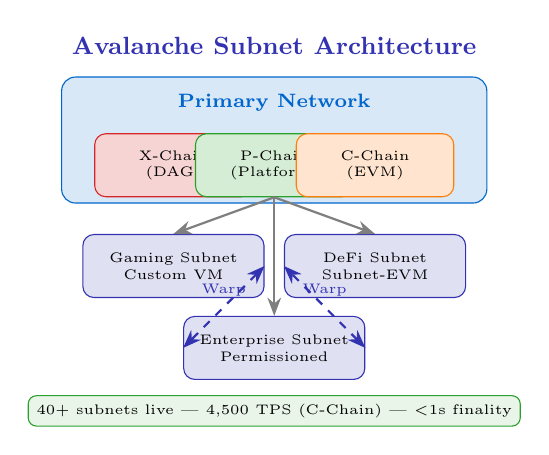
\begin{tikzpicture}[
  scale=0.80,
  every node/.style={font=\tiny},
  subbox/.style={draw,rounded corners=4pt,minimum width=2.0cm,minimum height=0.8cm,
                 align=center,inner sep=3pt},
]
  % Title
  \node[font=\small\bfseries,text=mlpurple] at (2.8,6.2) {Avalanche Subnet Architecture};

  % Primary network
  \node[draw,fill=mlblue!15,draw=mlblue,rounded corners=5pt,
        minimum width=5.4cm,minimum height=1.6cm,align=center] (pn) at (2.8,4.7) {};
  \node[font=\scriptsize\bfseries,text=mlblue] at (2.8,5.3) {Primary Network};

  \node[subbox,fill=mlred!20,draw=mlred] (xc) at (1.2,4.3) {X-Chain\\(DAG)};
  \node[subbox,fill=mlgreen!20,draw=mlgreen] (pc) at (2.8,4.3) {P-Chain\\(Platform)};
  \node[subbox,fill=mlorange!20,draw=mlorange] (cc) at (4.4,4.3) {C-Chain\\(EVM)};

  % Subnets
  \node[subbox,fill=mlpurple!15,draw=mlpurple,minimum width=2.3cm] (s1) at (1.2,2.7)
    {Gaming Subnet\\Custom VM};
  \node[subbox,fill=mlpurple!15,draw=mlpurple,minimum width=2.3cm] (s2) at (4.4,2.7)
    {DeFi Subnet\\Subnet-EVM};
  \node[subbox,fill=mlpurple!15,draw=mlpurple,minimum width=2.3cm] (s3) at (2.8,1.4)
    {Enterprise Subnet\\Permissioned};

  % Connections
  \draw[-{Stealth},thick,mlgray] (pc.south) -- (s1.north);
  \draw[-{Stealth},thick,mlgray] (pc.south) -- (s2.north);
  \draw[-{Stealth},thick,mlgray] (pc.south) -- (s3.north);

  % Warp messaging
  \draw[{Stealth}-{Stealth},dashed,mlpurple,thick] (s1.east) -- (s3.west)
    node[midway,above,font=\tiny] {Warp};
  \draw[{Stealth}-{Stealth},dashed,mlpurple,thick] (s3.east) -- (s2.west)
    node[midway,above,font=\tiny] {Warp};

  % Stats
  \node[draw,fill=mlgreen!10,draw=mlgreen,rounded corners=3pt,
        minimum width=5.4cm,align=center,font=\tiny,inner sep=3pt]
    at (2.8,0.4) {%
    40+ subnets live | 4,500 TPS (C-Chain) | $<$1s finality%
  };
\end{tikzpicture}
\end{columns}
\bottomnote{Avalanche subnets allow custom blockchain deployments with independent VMs and validators, connected via Warp messaging}
\end{frame}

% Frame 41: The Modular Blockchain Thesis
\begin{frame}{The Modular Blockchain Thesis}
\vspace{-1mm}
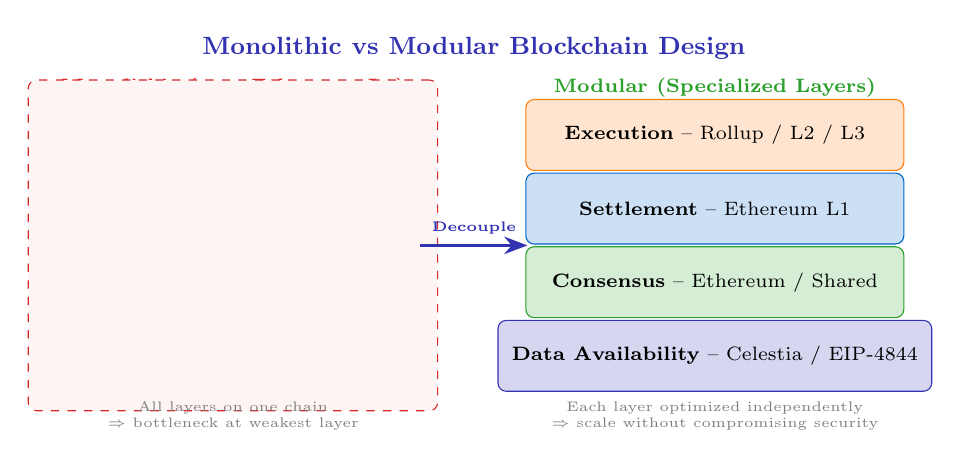
\begin{tikzpicture}[
  scale=0.85,
  every node/.style={font=\scriptsize},
  layerbox/.style={draw,rounded corners=3pt,minimum height=0.9cm,align=center,inner sep=5pt},
]
  % Title
  \node[font=\small\bfseries,text=mlpurple] at (6.6,6.3) {Monolithic vs Modular Blockchain Design};

  % Monolithic stack (left)
  \node[font=\scriptsize\bfseries,text=mlred] at (3.0,5.7) {Monolithic (e.g., Ethereum L1)};

  \node[layerbox,fill=mlred!20,draw=mlred,minimum width=4.8cm] (me) at (3.0,5.0)
    {\textbf{Execution} -- process transactions};
  \node[layerbox,fill=mlred!20,draw=mlred,minimum width=4.8cm] (ms) at (3.0,3.9)
    {\textbf{Settlement} -- finalize state};
  \node[layerbox,fill=mlred!20,draw=mlred,minimum width=4.8cm] (mc) at (3.0,2.8)
    {\textbf{Consensus} -- order transactions};
  \node[layerbox,fill=mlred!20,draw=mlred,minimum width=4.8cm] (md) at (3.0,1.7)
    {\textbf{Data Availability} -- store data};

  \node[draw,rounded corners=3pt,fill=mlred!5,draw=mlred,dashed,
        minimum width=5.2cm,minimum height=4.2cm] at (3.0,3.35) {};

  \node[font=\tiny,text=mlgray,align=center] at (3.0,0.8) {All layers on one chain\\$\Rightarrow$ bottleneck at weakest layer};

  % Modular stack (right)
  \node[font=\scriptsize\bfseries,text=mlgreen] at (10.2,5.7) {Modular (Specialized Layers)};

  \node[layerbox,fill=mlorange!20,draw=mlorange,minimum width=4.8cm] (re) at (10.2,5.0)
    {\textbf{Execution} -- Rollup / L2 / L3};
  \node[layerbox,fill=mlblue!20,draw=mlblue,minimum width=4.8cm] (rs) at (10.2,3.9)
    {\textbf{Settlement} -- Ethereum L1};
  \node[layerbox,fill=mlgreen!20,draw=mlgreen,minimum width=4.8cm] (rc) at (10.2,2.8)
    {\textbf{Consensus} -- Ethereum / Shared};
  \node[layerbox,fill=mlpurple!20,draw=mlpurple,minimum width=4.8cm] (rd) at (10.2,1.7)
    {\textbf{Data Availability} -- Celestia / EIP-4844};

  \node[font=\tiny,text=mlgray,align=center] at (10.2,0.8) {Each layer optimized independently\\$\Rightarrow$ scale without compromising security};

  % Arrow between
  \draw[-{Stealth},very thick,mlpurple] (5.8,3.35) -- (7.4,3.35)
    node[midway,above,font=\tiny\bfseries] {Decouple};
\end{tikzpicture}
\bottomnote{Modular blockchains separate execution, settlement, consensus, and data availability into specialized optimized layers}
\end{frame}

% Frame 42: Bridge Contract [FRAGILE]
\begin{frame}[fragile]{Bridge Contract}
\begin{columns}[T]
\column{0.50\textwidth}
\vspace{1mm}
\begin{lstlisting}[language=Solidity,caption={L1 Bridge: Lock Tokens}]
// L1 Bridge: Lock tokens
contract L1Bridge {
    mapping(bytes32 => bool)
        public processedDeposits;

    function deposit(
        address token,
        uint256 amount,
        address l2Recipient
    ) external {
        IERC20(token).transferFrom(
            msg.sender,
            address(this),
            amount
        );
        bytes32 depositHash =
            keccak256(abi.encode(
                token, amount,
                l2Recipient,
                block.number
            ));
        emit DepositInitiated(
            depositHash,
            token, amount,
            l2Recipient);
    }
}
\end{lstlisting}
\column{0.50\textwidth}
\vspace{2mm}
\begin{block}{Lock-and-Mint Mechanism}
\footnotesize
\begin{itemize}
  \item \textbf{L1 Lock}: User deposits tokens into the L1 bridge contract; tokens are held in escrow
  \item \textbf{L2 Mint}: Bridge relayer detects deposit event; L2 contract mints equivalent wrapped tokens
  \item \textbf{Withdraw}: Reverse -- burn wrapped tokens on L2, unlock originals on L1
  \item \textbf{Deposit hash}: Unique identifier prevents replay attacks
\end{itemize}
\end{block}
\vspace{2mm}
\begin{alertblock}{Bridge Risks}
\footnotesize
\begin{itemize}
  \item \textbf{Smart contract bugs}: Bridge contracts hold billions in TVL -- a single vulnerability is catastrophic
  \item \textbf{Validator compromise}: Trusted bridges rely on honest multisig or validator set
  \item \textbf{Censorship}: Bridge operators can freeze or censor withdrawals
  \item \textbf{Liquidity fragmentation}: Wrapped tokens $\neq$ native tokens across chains
\end{itemize}
\end{alertblock}
\end{columns}
\bottomnote{Lock-and-mint bridges are the most common cross-chain mechanism -- they hold billions in TVL and are prime targets for exploits}
\end{frame}

% Frame 43: EIP-4844 & Blob Transactions
\begin{frame}{EIP-4844 \& Blob Transactions}
\vspace{-1mm}
\begin{columns}[T]
\column{0.48\textwidth}
\begin{block}{Proto-Danksharding (EIP-4844)}
\footnotesize
\begin{itemize}\setlength\itemsep{3pt}
  \item \textbf{New transaction type}: Type-3 blob-carrying transactions
  \item \textbf{Blob size}: \textasciitilde128 KB per blob, up to 6 blobs per block
  \item \textbf{Separate fee market}: Blob gas price independent of execution gas
  \item \textbf{Pruned after \textasciitilde18 days}: Not permanently stored on-chain
  \item \textbf{Cost reduction}: 10--100$\times$ cheaper than calldata for L2s
\end{itemize}
\end{block}
\vspace{2mm}
\begin{block}{Impact on L2 Economics}
\footnotesize
\begin{itemize}
  \item Pre-4844: L2s paid \$0.10--\$1.00 per tx for calldata
  \item Post-4844: \$0.001--\$0.01 per tx via blobs
  \item \textbf{Target}: 3 blobs/block, max 6 blobs/block
  \item Blob fee adjusts via EIP-1559-style mechanism
  \item Launched \textbf{March 13, 2024} (Dencun upgrade)
\end{itemize}
\end{block}
\column{0.48\textwidth}
\vspace{1mm}
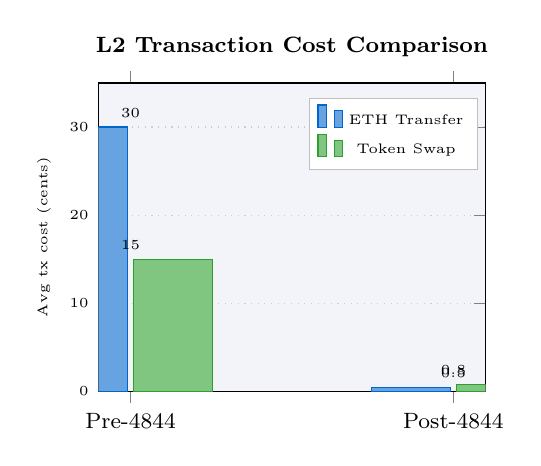
\begin{tikzpicture}
\begin{axis}[
  width=6.5cm,
  height=5.5cm,
  ybar,
  bar width=1.0cm,
  symbolic x coords={Pre-4844,Post-4844},
  xtick=data,
  xticklabel style={font=\footnotesize},
  yticklabel style={font=\tiny},
  ylabel={\tiny Avg tx cost (cents)},
  ylabel style={font=\tiny},
  title={\footnotesize L2 Transaction Cost Comparison},
  title style={font=\scriptsize\bfseries},
  ymin=0, ymax=35,
  ymajorgrids=true,
  grid style={dotted,mlgray!40},
  axis background/.style={fill=mllavender4!30},
  legend style={at={(0.98,0.95)},anchor=north east,font=\tiny,
                draw=mlgray!50,fill=white},
  nodes near coords,
  every node near coord/.style={font=\tiny},
]
  \addplot[fill=mlblue!60,draw=mlblue] coordinates
    {(Pre-4844, 30) (Post-4844, 0.5)};
  \addlegendentry{ETH Transfer}

  \addplot[fill=mlgreen!60,draw=mlgreen] coordinates
    {(Pre-4844, 15) (Post-4844, 0.8)};
  \addlegendentry{Token Swap}
\end{axis}
\end{tikzpicture}
\vspace{1mm}
\begin{center}
\footnotesize\textbf{Result:} L2 fees dropped \textasciitilde98\% post-Dencun
\end{center}
\end{columns}
\bottomnote{EIP-4844 introduced blob transactions (March 2024) -- a dedicated cheap data layer that reduced L2 costs by 10--100$\times$}
\end{frame}

% Frame 44: Celestia & Modular DA
\begin{frame}{Celestia \& Modular DA}
\vspace{-1mm}
\begin{columns}[T]
\column{0.48\textwidth}
\begin{block}{Celestia Architecture}
\footnotesize
\begin{itemize}\setlength\itemsep{3pt}
  \item \textbf{Purpose-built DA layer}: Only orders and publishes data -- no execution
  \item \textbf{Data Availability Sampling (DAS)}: Light nodes sample random chunks to verify availability
  \item \textbf{Namespaced Merkle Trees (NMTs)}: Each rollup reads only its own namespace
  \item \textbf{Throughput}: \textasciitilde6.67 MB/s data throughput target
  \item \textbf{Security model}: Honest majority of light nodes ensures DA
\end{itemize}
\end{block}
\vspace{2mm}
\begin{block}{DA vs Execution}
\footnotesize
\begin{itemize}
  \item Celestia provides \textbf{only data availability} -- no smart contracts, no execution
  \item Rollups post data to Celestia instead of (or in addition to) Ethereum
  \item Tradeoff: Cheaper DA but weaker security guarantees than Ethereum DA
  \item Sovereign rollups: Rollups that settle on Celestia without an L1 settlement layer
\end{itemize}
\end{block}
\column{0.48\textwidth}
\vspace{1mm}
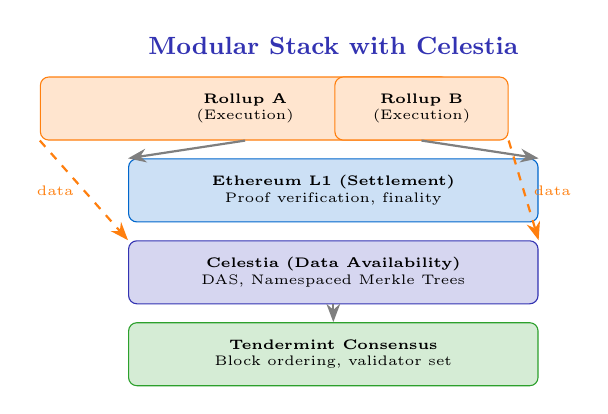
\begin{tikzpicture}[
  scale=0.80,
  every node/.style={font=\tiny},
  modbox/.style={draw,rounded corners=3pt,minimum width=5.2cm,minimum height=0.8cm,
                 align=center,inner sep=4pt},
]
  % Title
  \node[font=\small\bfseries,text=mlpurple] at (2.8,6.2) {Modular Stack with Celestia};

  % Execution layer
  \node[modbox,fill=mlorange!20,draw=mlorange] (ex1) at (1.4,5.2)
    {\textbf{Rollup A}\\(Execution)};
  \node[modbox,fill=mlorange!20,draw=mlorange,minimum width=2.2cm] (ex2) at (4.2,5.2)
    {\textbf{Rollup B}\\(Execution)};

  % Settlement
  \node[modbox,fill=mlblue!20,draw=mlblue] (se) at (2.8,3.9)
    {\textbf{Ethereum L1 (Settlement)}\\Proof verification, finality};

  % DA Layer
  \node[modbox,fill=mlpurple!20,draw=mlpurple] (da) at (2.8,2.6)
    {\textbf{Celestia (Data Availability)}\\DAS, Namespaced Merkle Trees};

  % Consensus
  \node[modbox,fill=mlgreen!20,draw=mlgreen] (cn) at (2.8,1.3)
    {\textbf{Tendermint Consensus}\\Block ordering, validator set};

  % Arrows
  \draw[-{Stealth},thick,mlgray] (ex1.south) -- (se.north west);
  \draw[-{Stealth},thick,mlgray] (ex2.south) -- (se.north east);
  \draw[-{Stealth},thick,mlorange,dashed] (ex1.south west) -- (da.north west)
    node[midway,left,font=\tiny] {data};
  \draw[-{Stealth},thick,mlorange,dashed] (ex2.south east) -- (da.north east)
    node[midway,right,font=\tiny] {data};
  \draw[-{Stealth},thick,mlgray] (da.south) -- (cn.north);
\end{tikzpicture}
\end{columns}
\bottomnote{Celestia is a purpose-built data availability layer -- rollups post data to Celestia for cheap DA while settling proofs on Ethereum}
\end{frame}

% Frame 45: Danksharding Roadmap
\begin{frame}{Danksharding Roadmap}
\vspace{-1mm}
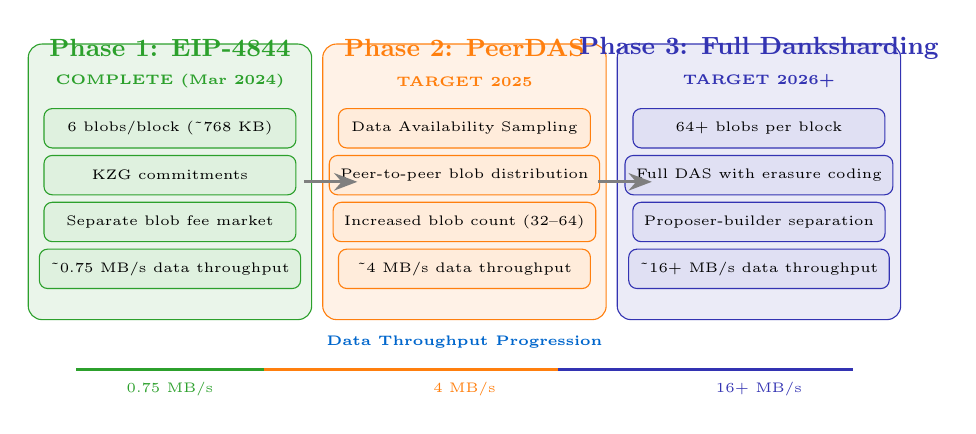
\begin{tikzpicture}[
  scale=0.85,
  every node/.style={font=\scriptsize},
  phasebox/.style={draw,rounded corners=5pt,minimum width=3.6cm,minimum height=3.5cm,
                   align=center,inner sep=6pt},
  detailbox/.style={draw,rounded corners=3pt,minimum width=3.2cm,minimum height=0.5cm,
                    align=left,inner sep=4pt,font=\tiny},
]
  % Phase 1: EIP-4844
  \node[phasebox,fill=mlgreen!10,draw=mlgreen] (p1) at (2.2,3.0) {};
  \node[font=\small\bfseries,text=mlgreen] at (2.2,5.0) {Phase 1: EIP-4844};
  \node[font=\tiny\bfseries,text=mlgreen] at (2.2,4.5) {COMPLETE (Mar 2024)};

  \node[detailbox,fill=mlgreen!15,draw=mlgreen] at (2.2,3.8)
    {6 blobs/block (\textasciitilde768 KB)};
  \node[detailbox,fill=mlgreen!15,draw=mlgreen] at (2.2,3.1)
    {KZG commitments};
  \node[detailbox,fill=mlgreen!15,draw=mlgreen] at (2.2,2.4)
    {Separate blob fee market};
  \node[detailbox,fill=mlgreen!15,draw=mlgreen] at (2.2,1.7)
    {\textasciitilde0.75 MB/s data throughput};

  % Phase 2: PeerDAS
  \node[phasebox,fill=mlorange!10,draw=mlorange] (p2) at (6.6,3.0) {};
  \node[font=\small\bfseries,text=mlorange] at (6.6,5.0) {Phase 2: PeerDAS};
  \node[font=\tiny\bfseries,text=mlorange] at (6.6,4.5) {TARGET 2025};

  \node[detailbox,fill=mlorange!15,draw=mlorange] at (6.6,3.8)
    {Data Availability Sampling};
  \node[detailbox,fill=mlorange!15,draw=mlorange] at (6.6,3.1)
    {Peer-to-peer blob distribution};
  \node[detailbox,fill=mlorange!15,draw=mlorange] at (6.6,2.4)
    {Increased blob count (32--64)};
  \node[detailbox,fill=mlorange!15,draw=mlorange] at (6.6,1.7)
    {\textasciitilde4 MB/s data throughput};

  % Phase 3: Full Danksharding
  \node[phasebox,fill=mlpurple!10,draw=mlpurple] (p3) at (11.0,3.0) {};
  \node[font=\small\bfseries,text=mlpurple] at (11.0,5.0) {Phase 3: Full Danksharding};
  \node[font=\tiny\bfseries,text=mlpurple] at (11.0,4.5) {TARGET 2026+};

  \node[detailbox,fill=mlpurple!15,draw=mlpurple] at (11.0,3.8)
    {64+ blobs per block};
  \node[detailbox,fill=mlpurple!15,draw=mlpurple] at (11.0,3.1)
    {Full DAS with erasure coding};
  \node[detailbox,fill=mlpurple!15,draw=mlpurple] at (11.0,2.4)
    {Proposer-builder separation};
  \node[detailbox,fill=mlpurple!15,draw=mlpurple] at (11.0,1.7)
    {\textasciitilde16+ MB/s data throughput};

  % Timeline arrows
  \draw[-{Stealth},very thick,mlgray] (4.2,3.0) -- (5.0,3.0);
  \draw[-{Stealth},very thick,mlgray] (8.6,3.0) -- (9.4,3.0);

  % Data throughput progression bar
  \node[font=\tiny\bfseries,text=mlblue] at (6.6,0.6) {Data Throughput Progression};
  \draw[very thick,mlgreen] (0.8,0.2) -- (3.6,0.2);
  \draw[very thick,mlorange] (3.6,0.2) -- (8.0,0.2);
  \draw[very thick,mlpurple] (8.0,0.2) -- (12.4,0.2);
  \node[font=\tiny,text=mlgreen] at (2.2,-0.1) {0.75 MB/s};
  \node[font=\tiny,text=mlorange] at (6.6,-0.1) {4 MB/s};
  \node[font=\tiny,text=mlpurple] at (11.0,-0.1) {16+ MB/s};
\end{tikzpicture}
\bottomnote{Danksharding is Ethereum's DA roadmap: EIP-4844 (done) $\rightarrow$ PeerDAS (2025) $\rightarrow$ Full Danksharding (2026+) with 20$\times$ more throughput}
\end{frame}

% Frame 46: Validiums & Volitions
\begin{frame}{Validiums \& Volitions}
\vspace{-1mm}
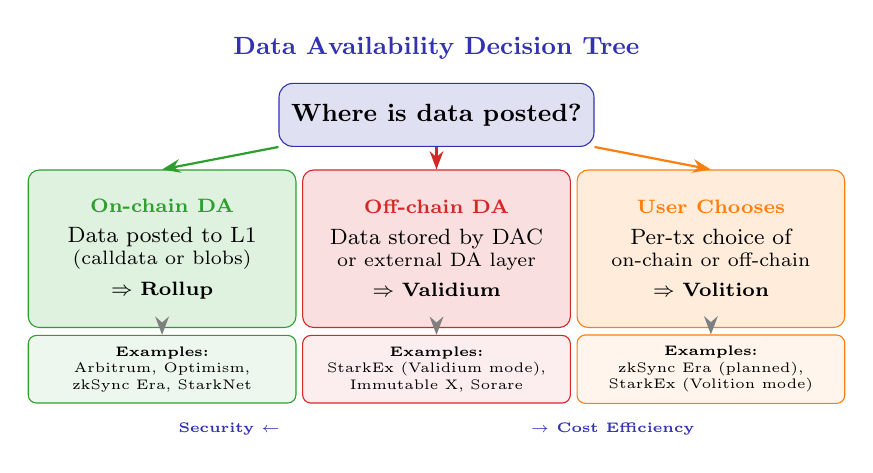
\begin{tikzpicture}[
  scale=0.85,
  every node/.style={font=\scriptsize},
  decbox/.style={draw,rounded corners=4pt,minimum width=3.4cm,minimum height=2.0cm,
                 align=center,inner sep=6pt},
]
  % Title
  \node[font=\small\bfseries,text=mlpurple] at (6.6,6.0) {Data Availability Decision Tree};

  % Root: Where is data stored?
  \node[draw,fill=mlpurple!15,draw=mlpurple,rounded corners=5pt,
        minimum width=4.0cm,minimum height=0.8cm,align=center,font=\small\bfseries]
    (root) at (6.6,5.0) {Where is data posted?};

  % Branch 1: On-chain DA
  \node[decbox,fill=mlgreen!15,draw=mlgreen] (onchain) at (2.5,3.0) {%
    \textbf{\textcolor{mlgreen}{On-chain DA}}\\[3pt]
    \footnotesize Data posted to L1\\
    (calldata or blobs)\\[3pt]
    $\Rightarrow$ \textbf{Rollup}
  };

  % Branch 2: Off-chain DA
  \node[decbox,fill=mlred!15,draw=mlred] (offchain) at (6.6,3.0) {%
    \textbf{\textcolor{mlred}{Off-chain DA}}\\[3pt]
    \footnotesize Data stored by DAC\\
    or external DA layer\\[3pt]
    $\Rightarrow$ \textbf{Validium}
  };

  % Branch 3: User choice
  \node[decbox,fill=mlorange!15,draw=mlorange] (userchoice) at (10.7,3.0) {%
    \textbf{\textcolor{mlorange}{User Chooses}}\\[3pt]
    \footnotesize Per-tx choice of\\
    on-chain or off-chain\\[3pt]
    $\Rightarrow$ \textbf{Volition}
  };

  % Arrows from root
  \draw[-{Stealth},thick,mlgreen] (root.south west) -- (onchain.north);
  \draw[-{Stealth},thick,mlred] (root.south) -- (offchain.north);
  \draw[-{Stealth},thick,mlorange] (root.south east) -- (userchoice.north);

  % Examples
  \node[draw,fill=mlgreen!8,draw=mlgreen,rounded corners=3pt,
        minimum width=3.4cm,align=center,font=\tiny,inner sep=4pt]
    (eg1) at (2.5,1.2) {%
    \textbf{Examples:}\\Arbitrum, Optimism,\\zkSync Era, StarkNet
  };
  \node[draw,fill=mlred!8,draw=mlred,rounded corners=3pt,
        minimum width=3.4cm,align=center,font=\tiny,inner sep=4pt]
    (eg2) at (6.6,1.2) {%
    \textbf{Examples:}\\StarkEx (Validium mode),\\Immutable X, Sorare
  };
  \node[draw,fill=mlorange!8,draw=mlorange,rounded corners=3pt,
        minimum width=3.4cm,align=center,font=\tiny,inner sep=4pt]
    (eg3) at (10.7,1.2) {%
    \textbf{Examples:}\\zkSync Era (planned),\\StarkEx (Volition mode)
  };

  % Connecting lines
  \draw[-{Stealth},thick,mlgray] (onchain.south) -- (eg1.north);
  \draw[-{Stealth},thick,mlgray] (offchain.south) -- (eg2.north);
  \draw[-{Stealth},thick,mlgray] (userchoice.south) -- (eg3.north);

  % Security spectrum bar
  \node[font=\tiny\bfseries,text=mlpurple] at (6.6,0.3) {Security $\leftarrow$ \hspace{3cm} $\rightarrow$ Cost Efficiency};
\end{tikzpicture}
\bottomnote{Rollups store data on-chain (max security); validiums store off-chain (cheaper); volitions let users choose per transaction}
\end{frame}

% Frame 47: Section 4 Summary
\begin{frame}{Section 4 Summary}
\vspace{2mm}
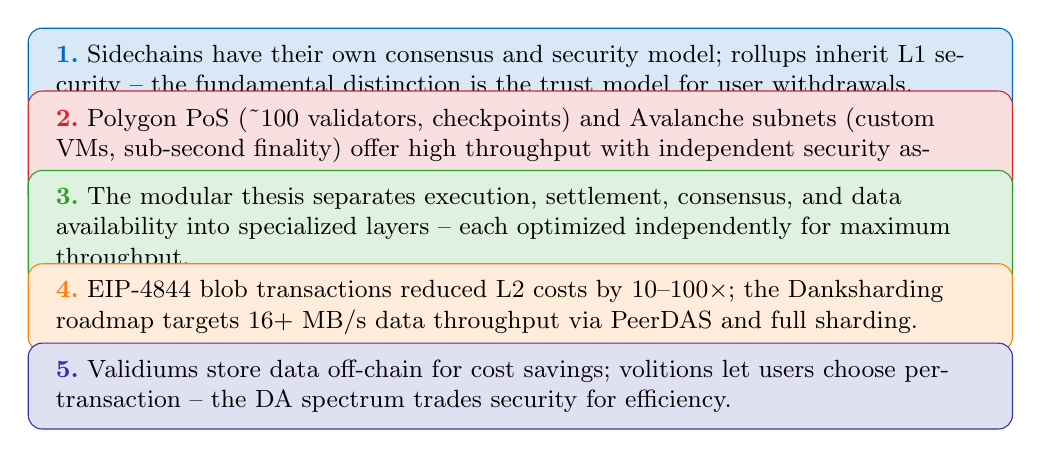
\begin{tikzpicture}[
  scale=1.0,
  every node/.style={font=\small},
  sumbox/.style={draw,rounded corners=5pt,minimum width=12.5cm,minimum height=0.85cm,
                 align=left,text width=11.8cm,inner sep=6pt},
]
  % Box 1
  \node[sumbox,fill=mlblue!15,draw=mlblue] (k1) at (6.5, 4.5) {%
    \textbf{\textcolor{mlblue}{1.}}~Sidechains have their own consensus and security model;
    rollups inherit L1 security -- the fundamental distinction is the trust model for user withdrawals.
  };
  % Box 2
  \node[sumbox,fill=mlred!15,draw=mlred] (k2) at (6.5, 3.5) {%
    \textbf{\textcolor{mlred}{2.}}~Polygon PoS (\textasciitilde100 validators, checkpoints) and Avalanche subnets
    (custom VMs, sub-second finality) offer high throughput with independent security assumptions.
  };
  % Box 3
  \node[sumbox,fill=mlgreen!15,draw=mlgreen] (k3) at (6.5, 2.5) {%
    \textbf{\textcolor{mlgreen}{3.}}~The modular thesis separates execution, settlement, consensus, and data availability
    into specialized layers -- each optimized independently for maximum throughput.
  };
  % Box 4
  \node[sumbox,fill=mlorange!15,draw=mlorange] (k4) at (6.5, 1.5) {%
    \textbf{\textcolor{mlorange}{4.}}~EIP-4844 blob transactions reduced L2 costs by 10--100$\times$;
    the Danksharding roadmap targets 16+ MB/s data throughput via PeerDAS and full sharding.
  };
  % Box 5
  \node[sumbox,fill=mlpurple!15,draw=mlpurple] (k5) at (6.5, 0.5) {%
    \textbf{\textcolor{mlpurple}{5.}}~Validiums store data off-chain for cost savings;
    volitions let users choose per-transaction -- the DA spectrum trades security for efficiency.
  };
\end{tikzpicture}
\bottomnote{Section 4 complete -- next: L2 Ecosystem \& Future (bridges, economics, L3s, account abstraction)}
\end{frame}

%% ============================================================
%% SECTION 5: L2 Ecosystem & Future
%% ============================================================
\section{L2 Ecosystem \& Future}

% Frame 48: Section 5 Divider
\begin{frame}{}
\vspace{10mm}
\begin{beamercolorbox}[sep=12pt,center,rounded=true,shadow=true]{palette quaternary}
{\Large\bfseries Section 5: L2 Ecosystem \& Future}\\[6pt]
{\normalsize Bridge security, L2 economics, L3s, and the rollup-centric roadmap}
\end{beamercolorbox}
\vspace{6mm}
\begin{columns}[T]
\begin{column}{0.48\textwidth}
\begin{block}{What You Will Learn}
\begin{itemize}\setlength\itemsep{3pt}
  \item[\small$\checkmark$] \small Bridge security vulnerabilities and major hack post-mortems
  \item[\small$\checkmark$] \small Cross-L2 communication: shared sequencing and intent protocols
  \item[\small$\checkmark$] \small L2 economics: sequencer revenue, MEV, and cost structures
  \item[\small$\checkmark$] \small L3s, account abstraction, and the rollup-centric endgame
\end{itemize}
\end{block}
\end{column}
\begin{column}{0.48\textwidth}
\begin{block}{Frames in This Section}
\begin{itemize}\setlength\itemsep{3pt}
  \item[\small$\bullet$] \small Frame 49: Bridge Security \& Major Hacks
  \item[\small$\bullet$] \small Frame 50: Cross-L2 Communication
  \item[\small$\bullet$] \small Frame 51: L2 Economics
  \item[\small$\bullet$] \small Frame 52: MEV on Layer 2
  \item[\small$\bullet$] \small Frame 53: L3s \& App-Specific Chains
  \item[\small$\bullet$] \small Frame 54: Account Abstraction on L2
  \item[\small$\bullet$] \small Frame 55: Key Takeaways and Course Summary
\end{itemize}
\end{block}
\end{column}
\end{columns}
\bottomnote{Section 5 of 5 -- L2 Ecosystem \& Future: the road ahead for Ethereum scaling}
\end{frame}

% Frame 49: Bridge Security & Major Hacks
\begin{frame}{Bridge Security \& Major Hacks}
\vspace{-1mm}
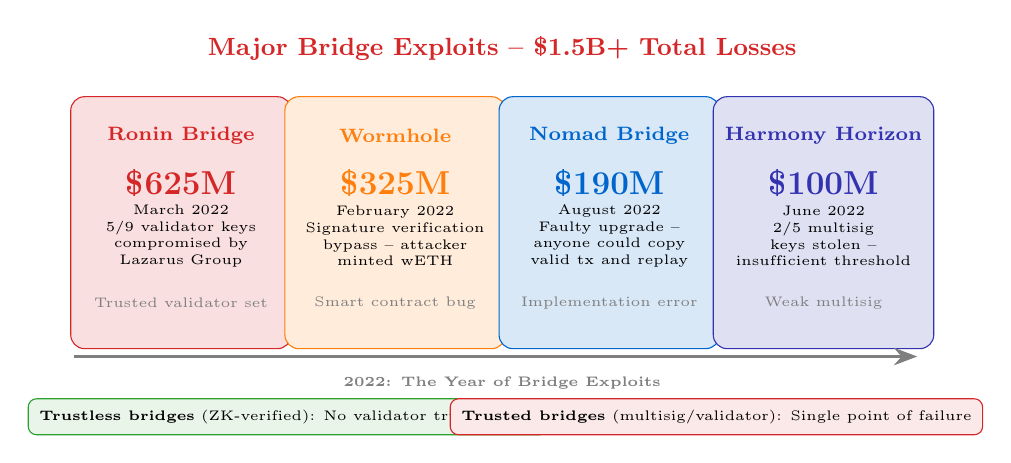
\begin{tikzpicture}[
  scale=0.85,
  every node/.style={font=\scriptsize},
  hackbox/.style={draw,rounded corners=5pt,minimum width=2.8cm,minimum height=3.2cm,
                  align=center,inner sep=5pt},
]
  % Title
  \node[font=\small\bfseries,text=mlred] at (6.6,5.8) {Major Bridge Exploits -- \$1.5B+ Total Losses};

  % Ronin
  \node[hackbox,fill=mlred!15,draw=mlred] (r1) at (1.8,3.2) {};
  \node[font=\scriptsize\bfseries,text=mlred] at (1.8,4.5) {Ronin Bridge};
  \node[font=\large\bfseries,text=mlred] at (1.8,3.8) {\$625M};
  \node[font=\tiny,align=center] at (1.8,3.0) {March 2022\\5/9 validator keys\\compromised by\\Lazarus Group};
  \node[font=\tiny,text=mlgray] at (1.8,2.0) {Trusted validator set};

  % Wormhole
  \node[hackbox,fill=mlorange!15,draw=mlorange] (r2) at (5.0,3.2) {};
  \node[font=\scriptsize\bfseries,text=mlorange] at (5.0,4.5) {Wormhole};
  \node[font=\large\bfseries,text=mlorange] at (5.0,3.8) {\$325M};
  \node[font=\tiny,align=center] at (5.0,3.0) {February 2022\\Signature verification\\bypass -- attacker\\minted wETH};
  \node[font=\tiny,text=mlgray] at (5.0,2.0) {Smart contract bug};

  % Nomad
  \node[hackbox,fill=mlblue!15,draw=mlblue] (r3) at (8.2,3.2) {};
  \node[font=\scriptsize\bfseries,text=mlblue] at (8.2,4.5) {Nomad Bridge};
  \node[font=\large\bfseries,text=mlblue] at (8.2,3.8) {\$190M};
  \node[font=\tiny,align=center] at (8.2,3.0) {August 2022\\Faulty upgrade --\\anyone could copy\\valid tx and replay};
  \node[font=\tiny,text=mlgray] at (8.2,2.0) {Implementation error};

  % Harmony
  \node[hackbox,fill=mlpurple!15,draw=mlpurple] (r4) at (11.4,3.2) {};
  \node[font=\scriptsize\bfseries,text=mlpurple] at (11.4,4.5) {Harmony Horizon};
  \node[font=\large\bfseries,text=mlpurple] at (11.4,3.8) {\$100M};
  \node[font=\tiny,align=center] at (11.4,3.0) {June 2022\\2/5 multisig\\keys stolen --\\insufficient threshold};
  \node[font=\tiny,text=mlgray] at (11.4,2.0) {Weak multisig};

  % Timeline arrow
  \draw[-{Stealth},very thick,mlgray] (0.2,1.2) -- (12.8,1.2);
  \node[font=\tiny\bfseries,text=mlgray] at (6.6,0.8) {2022: The Year of Bridge Exploits};

  % Trustless vs trusted
  \node[draw,fill=mlgreen!10,draw=mlgreen,rounded corners=3pt,
        minimum width=6.0cm,align=center,font=\tiny,inner sep=4pt]
    at (3.4,0.3) {%
    \textbf{Trustless bridges} (ZK-verified): No validator trust needed%
  };
  \node[draw,fill=mlred!10,draw=mlred,rounded corners=3pt,
        minimum width=6.0cm,align=center,font=\tiny,inner sep=4pt]
    at (9.8,0.3) {%
    \textbf{Trusted bridges} (multisig/validator): Single point of failure%
  };
\end{tikzpicture}
\bottomnote{Bridge exploits caused \$1.5B+ in losses in 2022 alone -- trustless ZK-verified bridges are the industry response to validator trust risks}
\end{frame}

% Frame 50: Cross-L2 Communication
\begin{frame}{Cross-L2 Communication}
\vspace{-1mm}
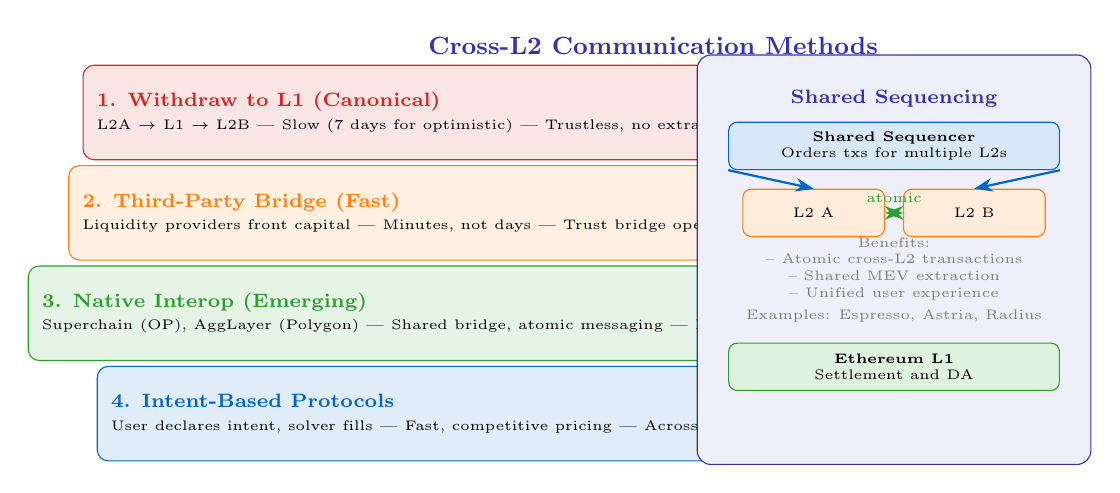
\begin{tikzpicture}[
  scale=0.85,
  every node/.style={font=\scriptsize},
  methbox/.style={draw,rounded corners=4pt,minimum width=5.8cm,minimum height=1.2cm,
                  align=left,inner sep=5pt},
]
  % Title
  \node[font=\small\bfseries,text=mlpurple] at (6.6,5.8) {Cross-L2 Communication Methods};

  % Method 1: Withdraw to L1
  \node[methbox,fill=mlred!12,draw=mlred] (m1) at (3.6,4.8) {%
    \textbf{\textcolor{mlred}{1. Withdraw to L1 (Canonical)}}\\
    \tiny L2A $\rightarrow$ L1 $\rightarrow$ L2B | Slow (7 days for optimistic) | Trustless, no extra assumptions
  };

  % Method 2: Third-party bridge
  \node[methbox,fill=mlorange!12,draw=mlorange] (m2) at (3.6,3.3) {%
    \textbf{\textcolor{mlorange}{2. Third-Party Bridge (Fast)}}\\
    \tiny Liquidity providers front capital | Minutes, not days | Trust bridge operator/liquidity
  };

  % Method 3: Native interop
  \node[methbox,fill=mlgreen!12,draw=mlgreen] (m3) at (3.6,1.8) {%
    \textbf{\textcolor{mlgreen}{3. Native Interop (Emerging)}}\\
    \tiny Superchain (OP), AggLayer (Polygon) | Shared bridge, atomic messaging | Requires same stack
  };

  % Method 4: Intent-based
  \node[methbox,fill=mlblue!12,draw=mlblue] (m4) at (3.6,0.3) {%
    \textbf{\textcolor{mlblue}{4. Intent-Based Protocols}}\\
    \tiny User declares intent, solver fills | Fast, competitive pricing | Across, UniswapX
  };

  % Right side: Shared sequencing concept
  \node[draw,fill=mlpurple!8,draw=mlpurple,rounded corners=5pt,
        minimum width=5.0cm,minimum height=5.2cm,align=center] at (10.2,2.6) {};
  \node[font=\scriptsize\bfseries,text=mlpurple] at (10.2,5.0) {Shared Sequencing};

  \node[draw,fill=mlblue!15,draw=mlblue,rounded corners=3pt,
        minimum width=4.2cm,minimum height=0.6cm,align=center,font=\tiny]
    (ss) at (10.2,4.3) {\textbf{Shared Sequencer}\\Orders txs for multiple L2s};

  \node[draw,fill=mlorange!15,draw=mlorange,rounded corners=3pt,
        minimum width=1.8cm,minimum height=0.6cm,align=center,font=\tiny]
    (l2a) at (9.0,3.3) {L2 A};
  \node[draw,fill=mlorange!15,draw=mlorange,rounded corners=3pt,
        minimum width=1.8cm,minimum height=0.6cm,align=center,font=\tiny]
    (l2b) at (11.4,3.3) {L2 B};

  \draw[-{Stealth},thick,mlblue] (ss.south west) -- (l2a.north);
  \draw[-{Stealth},thick,mlblue] (ss.south east) -- (l2b.north);
  \draw[{Stealth}-{Stealth},thick,dashed,mlgreen] (l2a.east) -- (l2b.west)
    node[midway,above,font=\tiny] {atomic};

  \node[font=\tiny,align=center,text=mlgray] at (10.2,2.3) {%
    Benefits:\\
    -- Atomic cross-L2 transactions\\
    -- Shared MEV extraction\\
    -- Unified user experience\\[2pt]
    Examples: Espresso, Astria, Radius
  };

  \node[draw,fill=mlgreen!15,draw=mlgreen,rounded corners=3pt,
        minimum width=4.2cm,minimum height=0.6cm,align=center,font=\tiny]
    at (10.2,1.0) {\textbf{Ethereum L1}\\Settlement and DA};
\end{tikzpicture}
\bottomnote{Cross-L2 communication ranges from slow canonical routes to fast intent-based protocols -- shared sequencing enables atomic cross-rollup transactions}
\end{frame}

% Frame 51: L2 Economics
\begin{frame}{L2 Economics}
\vspace{-1mm}
\begin{columns}[T]
\column{0.48\textwidth}
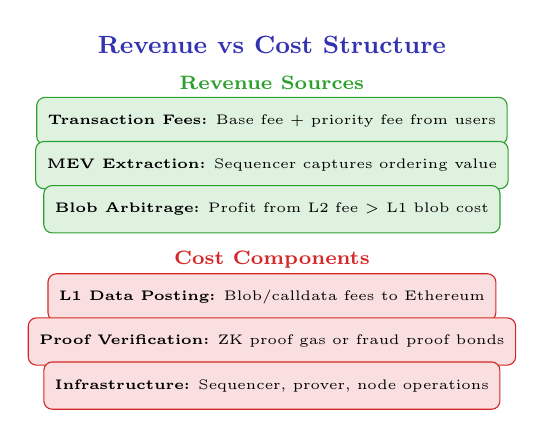
\begin{tikzpicture}[
  scale=0.80,
  every node/.style={font=\tiny},
  econbox/.style={draw,rounded corners=3pt,minimum width=5.2cm,minimum height=0.6cm,
                  align=left,inner sep=4pt},
]
  % Title
  \node[font=\small\bfseries,text=mlpurple] at (2.8,6.0) {Revenue vs Cost Structure};

  % Revenue side
  \node[font=\scriptsize\bfseries,text=mlgreen] at (2.8,5.4) {Revenue Sources};
  \node[econbox,fill=mlgreen!15,draw=mlgreen] at (2.8,4.8)
    {\textbf{Transaction Fees:} Base fee + priority fee from users};
  \node[econbox,fill=mlgreen!15,draw=mlgreen] at (2.8,4.1)
    {\textbf{MEV Extraction:} Sequencer captures ordering value};
  \node[econbox,fill=mlgreen!15,draw=mlgreen] at (2.8,3.4)
    {\textbf{Blob Arbitrage:} Profit from L2 fee $>$ L1 blob cost};

  % Cost side
  \node[font=\scriptsize\bfseries,text=mlred] at (2.8,2.6) {Cost Components};
  \node[econbox,fill=mlred!15,draw=mlred] at (2.8,2.0)
    {\textbf{L1 Data Posting:} Blob/calldata fees to Ethereum};
  \node[econbox,fill=mlred!15,draw=mlred] at (2.8,1.3)
    {\textbf{Proof Verification:} ZK proof gas or fraud proof bonds};
  \node[econbox,fill=mlred!15,draw=mlred] at (2.8,0.6)
    {\textbf{Infrastructure:} Sequencer, prover, node operations};
\end{tikzpicture}
\column{0.48\textwidth}
\vspace{1mm}
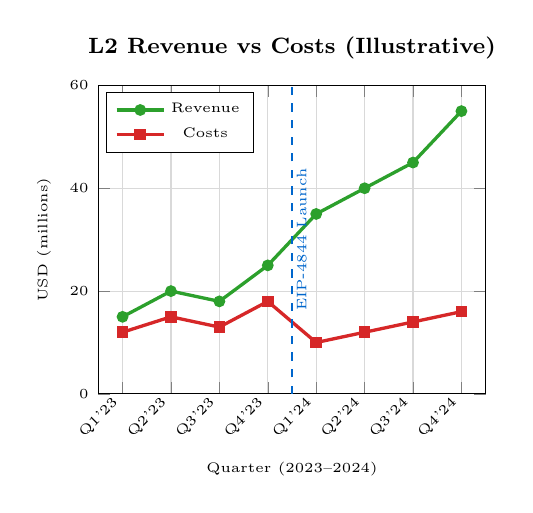
\begin{tikzpicture}
\begin{axis}[
  width=6.5cm,
  height=5.5cm,
  xlabel={Quarter (2023--2024)},
  ylabel={USD (millions)},
  title={\footnotesize L2 Revenue vs Costs (Illustrative)},
  title style={font=\scriptsize\bfseries},
  xmin=0.5, xmax=8.5,
  ymin=0, ymax=60,
  xtick={1,2,3,4,5,6,7,8},
  xticklabels={Q1'23,Q2'23,Q3'23,Q4'23,Q1'24,Q2'24,Q3'24,Q4'24},
  xticklabel style={font=\tiny,rotate=45,anchor=east},
  yticklabel style={font=\tiny},
  xlabel style={font=\tiny},
  ylabel style={font=\tiny},
  grid=major,
  grid style={mlgray!30},
  legend style={font=\tiny,at={(0.02,0.98)},anchor=north west},
]
  % Revenue
  \addplot[mlgreen,very thick,mark=*,mark size=1.5pt] coordinates
    {(1,15) (2,20) (3,18) (4,25) (5,35) (6,40) (7,45) (8,55)};
  \addlegendentry{Revenue}

  % Costs
  \addplot[mlred,very thick,mark=square*,mark size=1.5pt] coordinates
    {(1,12) (2,15) (3,13) (4,18) (5,10) (6,12) (7,14) (8,16)};
  \addlegendentry{Costs}

  % EIP-4844 annotation
  \draw[mlblue,dashed,thick] (axis cs:4.5,0) -- (axis cs:4.5,60);
  \node[font=\tiny,text=mlblue,rotate=90] at (axis cs:4.7,30) {EIP-4844 Launch};
\end{axis}
\end{tikzpicture}
\end{columns}
\bottomnote{L2 economics: revenue from fees and MEV vs costs of L1 data posting and proofs -- EIP-4844 dramatically improved margins}
\end{frame}

% Frame 52: MEV on Layer 2
\begin{frame}{MEV on Layer 2}
\vspace{-1mm}
\begin{columns}[T]
\column{0.48\textwidth}
\begin{block}{L2 MEV Context}
\footnotesize
\begin{itemize}\setlength\itemsep{3pt}
  \item \textbf{Sequencer monopoly}: Single sequencer controls transaction ordering -- no open mempool
  \item \textbf{MEV types}: Arbitrage, liquidations, sandwich attacks, NFT sniping
  \item \textbf{Scale}: Estimated \$100M+ annual MEV across major L2s
  \item \textbf{Fair ordering}: FCFS, encrypted mempools, MEV-sharing proposed
\end{itemize}
\end{block}
\vspace{2mm}
\begin{block}{Mitigation Approaches}
\footnotesize
\begin{itemize}
  \item \textbf{FCFS ordering}: Process transactions in arrival order (Arbitrum)
  \item \textbf{MEV-Share}: Return MEV to users via kickback mechanisms
  \item \textbf{Threshold encryption}: Encrypt txs until ordering is committed
  \item \textbf{Decentralized sequencing}: Remove single-party ordering power
\end{itemize}
\end{block}
\column{0.48\textwidth}
\vspace{1mm}
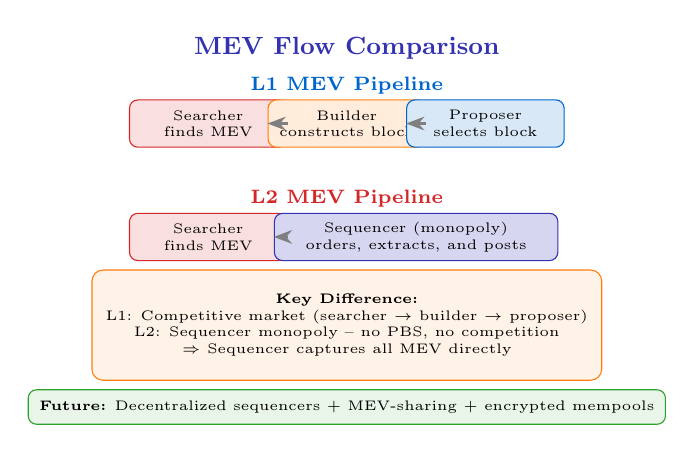
\begin{tikzpicture}[
  scale=0.80,
  every node/.style={font=\tiny},
  flowbox/.style={draw,rounded corners=3pt,minimum width=2.0cm,minimum height=0.6cm,
                  align=center,inner sep=3pt},
]
  % Title
  \node[font=\small\bfseries,text=mlpurple] at (2.8,6.2) {MEV Flow Comparison};

  % L1 MEV (top)
  \node[font=\scriptsize\bfseries,text=mlblue] at (2.8,5.6) {L1 MEV Pipeline};
  \node[flowbox,fill=mlred!15,draw=mlred] (s1) at (0.6,5.0) {Searcher\\finds MEV};
  \node[flowbox,fill=mlorange!15,draw=mlorange] (b1) at (2.8,5.0) {Builder\\constructs block};
  \node[flowbox,fill=mlblue!15,draw=mlblue] (p1) at (5.0,5.0) {Proposer\\selects block};

  \draw[-{Stealth},thick,mlgray] (s1.east) -- (b1.west);
  \draw[-{Stealth},thick,mlgray] (b1.east) -- (p1.west);

  % L2 MEV (bottom)
  \node[font=\scriptsize\bfseries,text=mlred] at (2.8,3.8) {L2 MEV Pipeline};
  \node[flowbox,fill=mlred!15,draw=mlred] (s2) at (0.6,3.2) {Searcher\\finds MEV};
  \node[flowbox,fill=mlpurple!20,draw=mlpurple,minimum width=3.6cm] (sq) at (3.9,3.2)
    {Sequencer (monopoly)\\orders, extracts, and posts};

  \draw[-{Stealth},thick,mlgray] (s2.east) -- (sq.west);

  % Key difference
  \node[draw,fill=mlorange!10,draw=mlorange,rounded corners=4pt,
        minimum width=5.0cm,minimum height=1.4cm,align=center,font=\tiny,inner sep=5pt]
    at (2.8,1.8) {%
    \textbf{Key Difference:}\\
    L1: Competitive market (searcher $\rightarrow$ builder $\rightarrow$ proposer)\\
    L2: Sequencer monopoly -- no PBS, no competition\\
    $\Rightarrow$ Sequencer captures all MEV directly%
  };

  % Future
  \node[draw,fill=mlgreen!10,draw=mlgreen,rounded corners=3pt,
        minimum width=5.0cm,align=center,font=\tiny,inner sep=4pt]
    at (2.8,0.5) {%
    \textbf{Future:} Decentralized sequencers + MEV-sharing + encrypted mempools%
  };
\end{tikzpicture}
\end{columns}
\bottomnote{L2 sequencers hold monopoly over transaction ordering and MEV extraction -- decentralized sequencing and fair ordering are active research areas}
\end{frame}

% Frame 53: L3s & App-Specific Chains
\begin{frame}{L3s \& App-Specific Chains}
\vspace{-1mm}
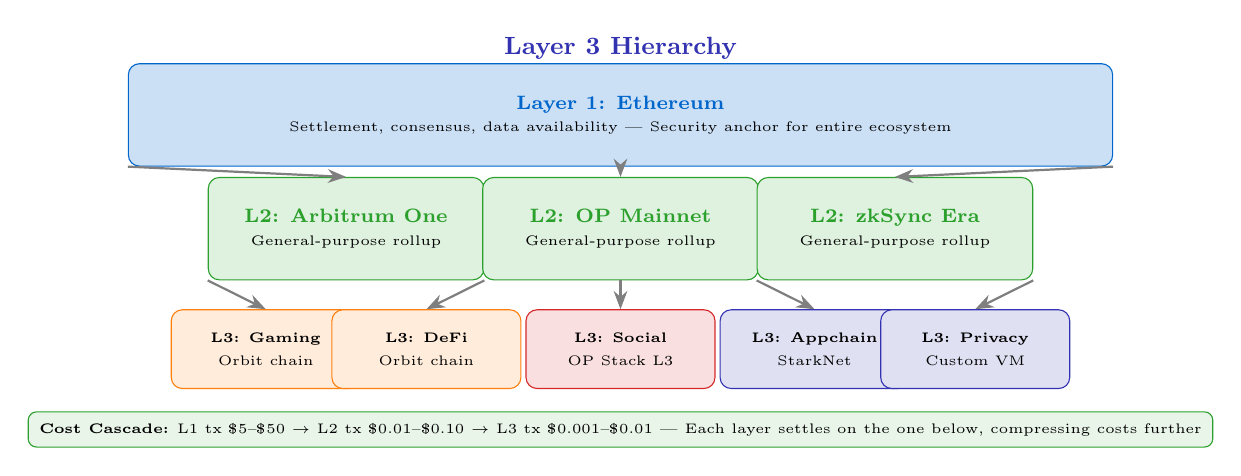
\begin{tikzpicture}[
  scale=0.85,
  every node/.style={font=\scriptsize},
  tierbox/.style={draw,rounded corners=4pt,minimum height=1.3cm,align=center,inner sep=6pt},
]
  % Title
  \node[font=\small\bfseries,text=mlpurple] at (6.6,6.0) {Layer 3 Hierarchy};

  % L1: Ethereum
  \node[tierbox,fill=mlblue!20,draw=mlblue,minimum width=12.5cm] (l1) at (6.6,5.0) {%
    \textbf{\textcolor{mlblue}{Layer 1: Ethereum}}\\
    \tiny Settlement, consensus, data availability | Security anchor for entire ecosystem
  };

  % L2: General rollups
  \node[tierbox,fill=mlgreen!15,draw=mlgreen,minimum width=3.5cm] (l2a) at (2.5,3.3) {%
    \textbf{\textcolor{mlgreen}{L2: Arbitrum One}}\\
    \tiny General-purpose rollup
  };
  \node[tierbox,fill=mlgreen!15,draw=mlgreen,minimum width=3.5cm] (l2b) at (6.6,3.3) {%
    \textbf{\textcolor{mlgreen}{L2: OP Mainnet}}\\
    \tiny General-purpose rollup
  };
  \node[tierbox,fill=mlgreen!15,draw=mlgreen,minimum width=3.5cm] (l2c) at (10.7,3.3) {%
    \textbf{\textcolor{mlgreen}{L2: zkSync Era}}\\
    \tiny General-purpose rollup
  };

  % L3: App-specific
  \node[tierbox,fill=mlorange!15,draw=mlorange,minimum width=2.4cm,minimum height=1.0cm] (l3a) at (1.3,1.5) {%
    \textbf{\tiny L3: Gaming}\\
    \tiny Orbit chain
  };
  \node[tierbox,fill=mlorange!15,draw=mlorange,minimum width=2.4cm,minimum height=1.0cm] (l3b) at (3.7,1.5) {%
    \textbf{\tiny L3: DeFi}\\
    \tiny Orbit chain
  };
  \node[tierbox,fill=mlred!15,draw=mlred,minimum width=2.4cm,minimum height=1.0cm] (l3c) at (6.6,1.5) {%
    \textbf{\tiny L3: Social}\\
    \tiny OP Stack L3
  };
  \node[tierbox,fill=mlpurple!15,draw=mlpurple,minimum width=2.4cm,minimum height=1.0cm] (l3d) at (9.5,1.5) {%
    \textbf{\tiny L3: Appchain}\\
    \tiny StarkNet
  };
  \node[tierbox,fill=mlpurple!15,draw=mlpurple,minimum width=2.4cm,minimum height=1.0cm] (l3e) at (11.9,1.5) {%
    \textbf{\tiny L3: Privacy}\\
    \tiny Custom VM
  };

  % Arrows
  \draw[-{Stealth},thick,mlgray] (l1.south west) -- (l2a.north);
  \draw[-{Stealth},thick,mlgray] (l1.south) -- (l2b.north);
  \draw[-{Stealth},thick,mlgray] (l1.south east) -- (l2c.north);

  \draw[-{Stealth},thick,mlgray] (l2a.south west) -- (l3a.north);
  \draw[-{Stealth},thick,mlgray] (l2a.south east) -- (l3b.north);
  \draw[-{Stealth},thick,mlgray] (l2b.south) -- (l3c.north);
  \draw[-{Stealth},thick,mlgray] (l2c.south west) -- (l3d.north);
  \draw[-{Stealth},thick,mlgray] (l2c.south east) -- (l3e.north);

  % Cost cascade
  \node[draw,fill=mlgreen!10,draw=mlgreen,rounded corners=3pt,
        minimum width=12.5cm,align=center,font=\tiny,inner sep=4pt]
    at (6.6,0.3) {%
    \textbf{Cost Cascade:} L1 tx \$5--\$50 $\rightarrow$ L2 tx \$0.01--\$0.10 $\rightarrow$ L3 tx \$0.001--\$0.01 |
    Each layer settles on the one below, compressing costs further%
  };
\end{tikzpicture}
\bottomnote{L3s settle on L2s (which settle on L1) -- app-specific chains via Orbit, OP Stack, or StarkNet Appchains for ultra-low-cost domain-specific execution}
\end{frame}

% Frame 54: Account Abstraction on L2
\begin{frame}{Account Abstraction on L2}
\vspace{-1mm}
\begin{columns}[T]
\column{0.48\textwidth}
\begin{block}{What is Account Abstraction?}
\footnotesize
\begin{itemize}\setlength\itemsep{3pt}
  \item \textbf{ERC-4337}: Smart contract wallets as first-class accounts (L1 standard)
  \item \textbf{Native AA}: Built into the protocol (zkSync Era, StarkNet)
  \item \textbf{Key insight}: Every account is a smart contract -- programmable validation logic
\end{itemize}
\end{block}
\vspace{2mm}
\begin{block}{Benefits for Users}
\footnotesize
\begin{itemize}\setlength\itemsep{3pt}
  \item \textbf{Gasless transactions}: Paymasters sponsor gas on behalf of users
  \item \textbf{Social recovery}: Recover wallet via trusted contacts (no seed phrase)
  \item \textbf{Session keys}: Time-limited keys for dApps (no per-tx signing)
  \item \textbf{Batched operations}: Multiple actions in a single transaction
  \item \textbf{Multi-sig built-in}: Require N-of-M signatures natively
\end{itemize}
\end{block}
\column{0.48\textwidth}
\vspace{1mm}
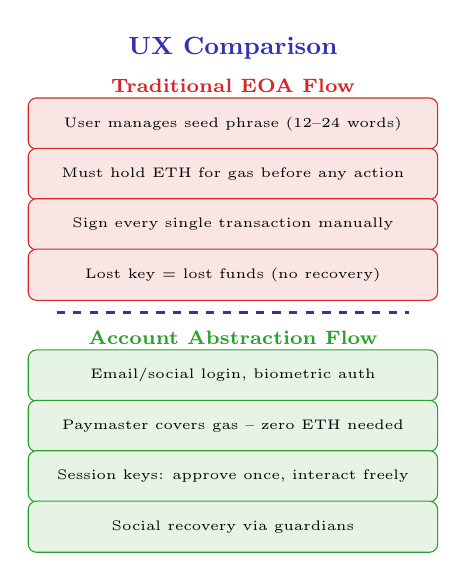
\begin{tikzpicture}[
  scale=0.80,
  every node/.style={font=\tiny},
  uxbox/.style={draw,rounded corners=3pt,minimum width=5.2cm,minimum height=0.65cm,
                align=center,inner sep=4pt},
]
  % Title
  \node[font=\small\bfseries,text=mlpurple] at (2.8,6.2) {UX Comparison};

  % Traditional flow
  \node[font=\scriptsize\bfseries,text=mlred] at (2.8,5.6) {Traditional EOA Flow};
  \node[uxbox,fill=mlred!12,draw=mlred] at (2.8,5.0) {User manages seed phrase (12--24 words)};
  \node[uxbox,fill=mlred!12,draw=mlred] at (2.8,4.2) {Must hold ETH for gas before any action};
  \node[uxbox,fill=mlred!12,draw=mlred] at (2.8,3.4) {Sign every single transaction manually};
  \node[uxbox,fill=mlred!12,draw=mlred] at (2.8,2.6) {Lost key = lost funds (no recovery)};

  % Divider
  \draw[mlpurple,thick,dashed] (0.0,2.0) -- (5.6,2.0);

  % AA flow
  \node[font=\scriptsize\bfseries,text=mlgreen] at (2.8,1.6) {Account Abstraction Flow};
  \node[uxbox,fill=mlgreen!12,draw=mlgreen] at (2.8,1.0) {Email/social login, biometric auth};
  \node[uxbox,fill=mlgreen!12,draw=mlgreen] at (2.8,0.2) {Paymaster covers gas -- zero ETH needed};
  \node[uxbox,fill=mlgreen!12,draw=mlgreen] at (2.8,-0.6) {Session keys: approve once, interact freely};
  \node[uxbox,fill=mlgreen!12,draw=mlgreen] at (2.8,-1.4) {Social recovery via guardians};
\end{tikzpicture}
\end{columns}
\bottomnote{Account abstraction transforms L2 UX: gasless txs, social recovery, session keys -- L2s with native AA (zkSync, StarkNet) lead adoption}
\end{frame}

% Frame 55: Key Takeaways and Course Summary
\begin{frame}{Key Takeaways and Course Summary}
\vspace{1mm}
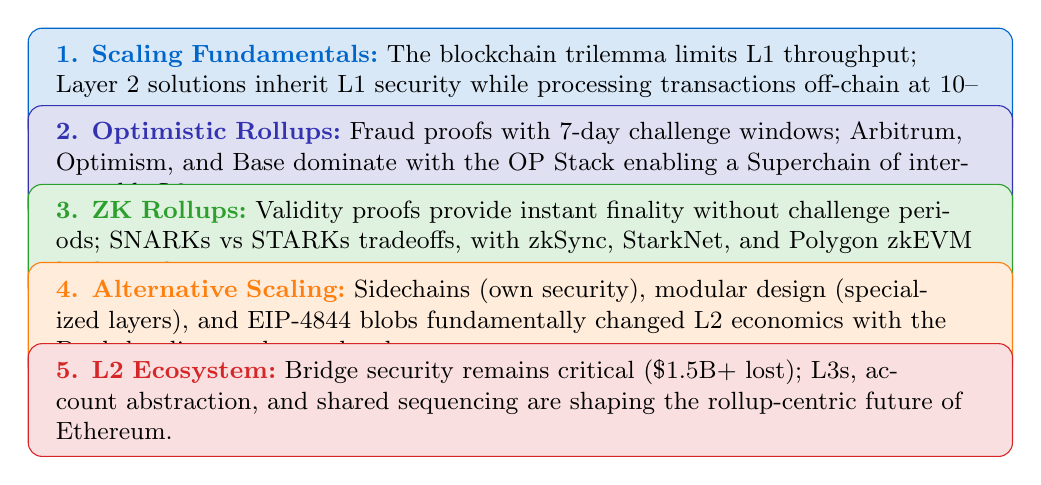
\begin{tikzpicture}[
  scale=1.0,
  every node/.style={font=\small},
  sumbox/.style={draw,rounded corners=5pt,minimum width=12.5cm,minimum height=0.85cm,
                 align=left,text width=11.8cm,inner sep=6pt},
]
  % Box 1: Section 1
  \node[sumbox,fill=mlblue!15,draw=mlblue] (k1) at (6.5, 4.5) {%
    \textbf{\textcolor{mlblue}{1. Scaling Fundamentals:}}~The blockchain trilemma limits L1 throughput;
    Layer 2 solutions inherit L1 security while processing transactions off-chain at 10--100$\times$ lower cost.
  };
  % Box 2: Section 2
  \node[sumbox,fill=mlpurple!15,draw=mlpurple] (k2) at (6.5, 3.5) {%
    \textbf{\textcolor{mlpurple}{2. Optimistic Rollups:}}~Fraud proofs with 7-day challenge windows;
    Arbitrum, Optimism, and Base dominate with the OP Stack enabling a Superchain of interoperable L2s.
  };
  % Box 3: Section 3
  \node[sumbox,fill=mlgreen!15,draw=mlgreen] (k3) at (6.5, 2.5) {%
    \textbf{\textcolor{mlgreen}{3. ZK Rollups:}}~Validity proofs provide instant finality without challenge periods;
    SNARKs vs STARKs tradeoffs, with zkSync, StarkNet, and Polygon zkEVM leading adoption.
  };
  % Box 4: Section 4
  \node[sumbox,fill=mlorange!15,draw=mlorange] (k4) at (6.5, 1.5) {%
    \textbf{\textcolor{mlorange}{4. Alternative Scaling:}}~Sidechains (own security), modular design (specialized layers),
    and EIP-4844 blobs fundamentally changed L2 economics with the Danksharding roadmap ahead.
  };
  % Box 5: Section 5
  \node[sumbox,fill=mlred!15,draw=mlred] (k5) at (6.5, 0.5) {%
    \textbf{\textcolor{mlred}{5. L2 Ecosystem:}}~Bridge security remains critical (\$1.5B+ lost);
    L3s, account abstraction, and shared sequencing are shaping the rollup-centric future of Ethereum.
  };
\end{tikzpicture}
\vspace{1mm}
\begin{beamercolorbox}[sep=6pt,center,rounded=true]{palette tertiary}
  \footnotesize\bfseries Next: Advanced topics in cross-chain interoperability, shared sequencing, and based rollups
\end{beamercolorbox}
\bottomnote{Course complete -- 5 sections, 55 frames | The rollup-centric roadmap is Ethereum's path to global-scale decentralized computation}
\end{frame}

\end{document}
